%!TEX root=./LIVRO.tex
\chapter{O que eu penso também tem valor}
\markboth{Módulo 1}{}

\section{Habilidades do SAEB}
\begin{itemize}
\item Identificar o uso de recursos persuasivos em textos verbais e não
  verbais.
\item Identificar teses, opiniões, posicionamentos explícitos e argumentos
  em textos.
\end{itemize}

\subsection{Habilidades da BNCC}
\begin{itemize}
\item EF67LP05
\item EF67LP07
\end{itemize}

\conteudo{Com frequência, no dia a dia, nos deparamos com informações de
diferentes tipos, que influenciam nosso modo de pensar ou de agir. Da
mesma forma, é comum que outras pessoas precisem exercer seu
posicionamento a respeito de determinados assuntos, a fim de fazer valer
aquilo que consideram ser mais apropriado.

Mas será que existe uma única forma de se expressar? Qual é a maneira
mais adequada de expressar um ponto de vista? Quais recursos devem ser
usados para dar credibilidade aos nossos argumentos?

Primeiramente, vamos retomar um conceito importante: por definição,
\textbf{argumentar} significa relacionar fatos, teses, estudos,
opiniões, problemas e possíveis soluções a fim de embasar determinado
pensamento ou ideia.

Sendo assim, para que uma ideia ou teoria seja considerada plausível, ou
seja, correta, é fundamental que ela esteja apoiada em aspectos
\textbf{lógicos}, e não apenas em aspectos \textbf{emotivos}. Isso quer
dizer que quando um ponto de vista é fornecido apenas com base na
emoção, ele pode ser facilmente contestado. Por outro lado, quando uma
teoria é apresentada a partir de aspectos lógicos, isto é, apoiados na
palavra de especialistas, em pesquisas e coletas de dados, por exemplo,
ela se torna forte o suficiente para servir, inclusive, como ponto de
referência.}

\pagebreak

\section{Atividades}

Leia o texto a seguir e responda às questões de 1 a 4.

\begin{quote}
\centering\textbf{Estudantes escrevem carta com sugestões para a cidade e entregam
ao prefeito}


As ideias de pequenos cidadãos parecem simples, mas podem resultar em
melhorias para a cidade. Estudantes da turma do 3º ano A, da Escola
Municipal de Ensino Fundamental (Emef) Octacílio Lomba, em Maruípe,
entregaram uma carta ao prefeito de Vitória, Lorenzo Pazolini, com
sugestões para a capital.

Além da escrita, feita a muitos pares de mãos, os estudantes também
fizeram desenhos sobre como está a situação hoje e como eles imaginam
que possa ser, com melhorias. No encontro com o prefeito, os estudantes
leram a carta.

``Percebemos que a rua da nossa escola alaga, às vezes. E isso tem nos
preocupado devido ao contato com vírus e bactérias que pode haver na
água do esgoto. Nós aprendemos que esses alagamentos acontecem devido ao
lixo que as pessoas jogam na rua. Será que o senhor não poderia investir
mais em trabalhos de conscientização da coleta seletiva? Assim as
pessoas vão aprender como o lixo deve ser organizado'', diz um dos
trechos da carta. {[}\ldots{}{]}

O amor pelos animais também foi um tópico tratado na carta: ``Se não for
pedir muito, o senhor poderia providenciar campanhas de conscientização
para evitar os maus tratos de animais? Pois eles também têm
sentimentos.'' {[}\ldots{}{]}

\fonte{Brunella França. Prefeitura de Vitória. Estudantes escrevem carta com
sugestões para a cidade e entregam ao prefeito. Disponível em: www.vitoria.es.gov.br/noticia/estudantes-escrevem-carta-com-sugestoes-para-a-cidade-e-entregam-ao-prefeito-44202.
Acesso em: 14 fev. 2023. Adaptado.}
\end{quote}

\begin{figure}[H]

%PORT_6_IMG-2 — POR.tex:90
\centering\includegraphics[width=\textwidth]{./imgSAEB_6_POR/freepik/PORT_6_IMG-2.jpeg}

\end{figure}

\num{1} O texto noticia a redação de uma carta de reclamação, por parte
de estudantes de uma escola municipal de Maruípe, em Vitória (ES),
destinada ao prefeito da cidade. Qual é o objetivo da carta?

\reduline{O objetivo era demonstrar situações preocupantes no município,
do ponto de vista dos alunos, além de sugestões de melhoria propostas por
eles.\hfill}\linhas{1}

\num{2} Qual argumento os(as) estudantes utilizam para justificar sua
preocupação com os alagamentos na escola? De que maneira eles(as) sabem
desse tipo de informação?

\reduline{Os(as) estudantes se preocupam com os vírus e bactérias que
podem estar presentes na água do esgoto. Segundo a carta, eles
aprenderam que esses alagamentos acontecem devido ao lixo que as pessoas
jogam na rua.\hfill}\linhas{1}

\num{3} Qual é a tese proposta pelos(as) estudantes como possível
solução para os alagamentos na escola? O que justifica essa escolha?

\reduline{Os(as) estudantes propõem que o prefeito invista em
conscientização sobre coleta seletiva, pois, dessa forma, as pessoas
saberiam melhor a destinação do lixo, reduzindo a possibilidade de o
jogarem incorretamente na rua.\hfill}\linhas{1}

\num{4} No último parágrafo, a jornalista afirma que ``o amor pelos
animais também foi um tópico tratado na carta''. Com base na leitura
desse parágrafo, é possível afirmar que a solicitação dos(as) estudantes
foi feita com base em um argumento lógico ou emotivo? Justifique sua
resposta.

\reduline{Pode-se afirmar que a solicitação dos(as) estudantes foi feita
com base em um argumento emotivo, uma vez que afirmam na carta que os
animais também têm sentimentos, mas não apresentam nenhum argumento
lógico, como pesquisa científica ou palavra de especialista, que
justifique esse argumento.\hfill}\linhas{1}

\noindent\textbf{A resenha crítica é um tipo de texto que tem por característica
avaliar obras dos mais diversos tipos: artigos, livros, canções, peças
teatrais, filmes etc. Leia a seguir um trecho da resenha crítica do
filme \emph{Turma da Mônica: Laços} e responda às questões 5, 6 e 7.}


\begin{quote}
A adaptação cinematográfica de \emph{Turma da Mônica: Laços} apresenta
uma estética visual incrivelmente colorida, que serve como base para uma
história que enfatiza a importância da amizade acima das diferenças.

O filme preserva a inocência das crianças, que corajosamente se
aventuram em um lugar proibido em busca de seu amigo peludo, que está
sob a custódia de uma figura misteriosa. No entanto, a ingenuidade delas
tem seus limites e não é exagerada, o que retrata a infância sem tornar
os personagens bobos ou pouco realistas.

Daniel Rezende, que já demonstrou suas habilidades como diretor em
\emph{Bingo: O Rei das Manhãs} (2017), presta uma preciosa homenagem à
imaginação de Maurício de Sousa neste seu segundo longa-metragem. Ao
mesmo tempo, resgata uma infância com um toque nostálgico do passado, um
período marcado por questões atemporais, sem a presença de dispositivos
eletrônicos ou qualquer outra distração moderna.

\fonte{Marcelo Müller. Papo de Cinema. \emph{Resenha crítica de
Turma da Mônica: Laços}. Disponível em: https://www.papodecinema.com.br/filmes/turma-da-monica-lacos. Acesso em: 22 fev. 2023.}
\end{quote}


\begin{figure}[H]
%PORT_6_IMG-3 — POR.tex:163
\centering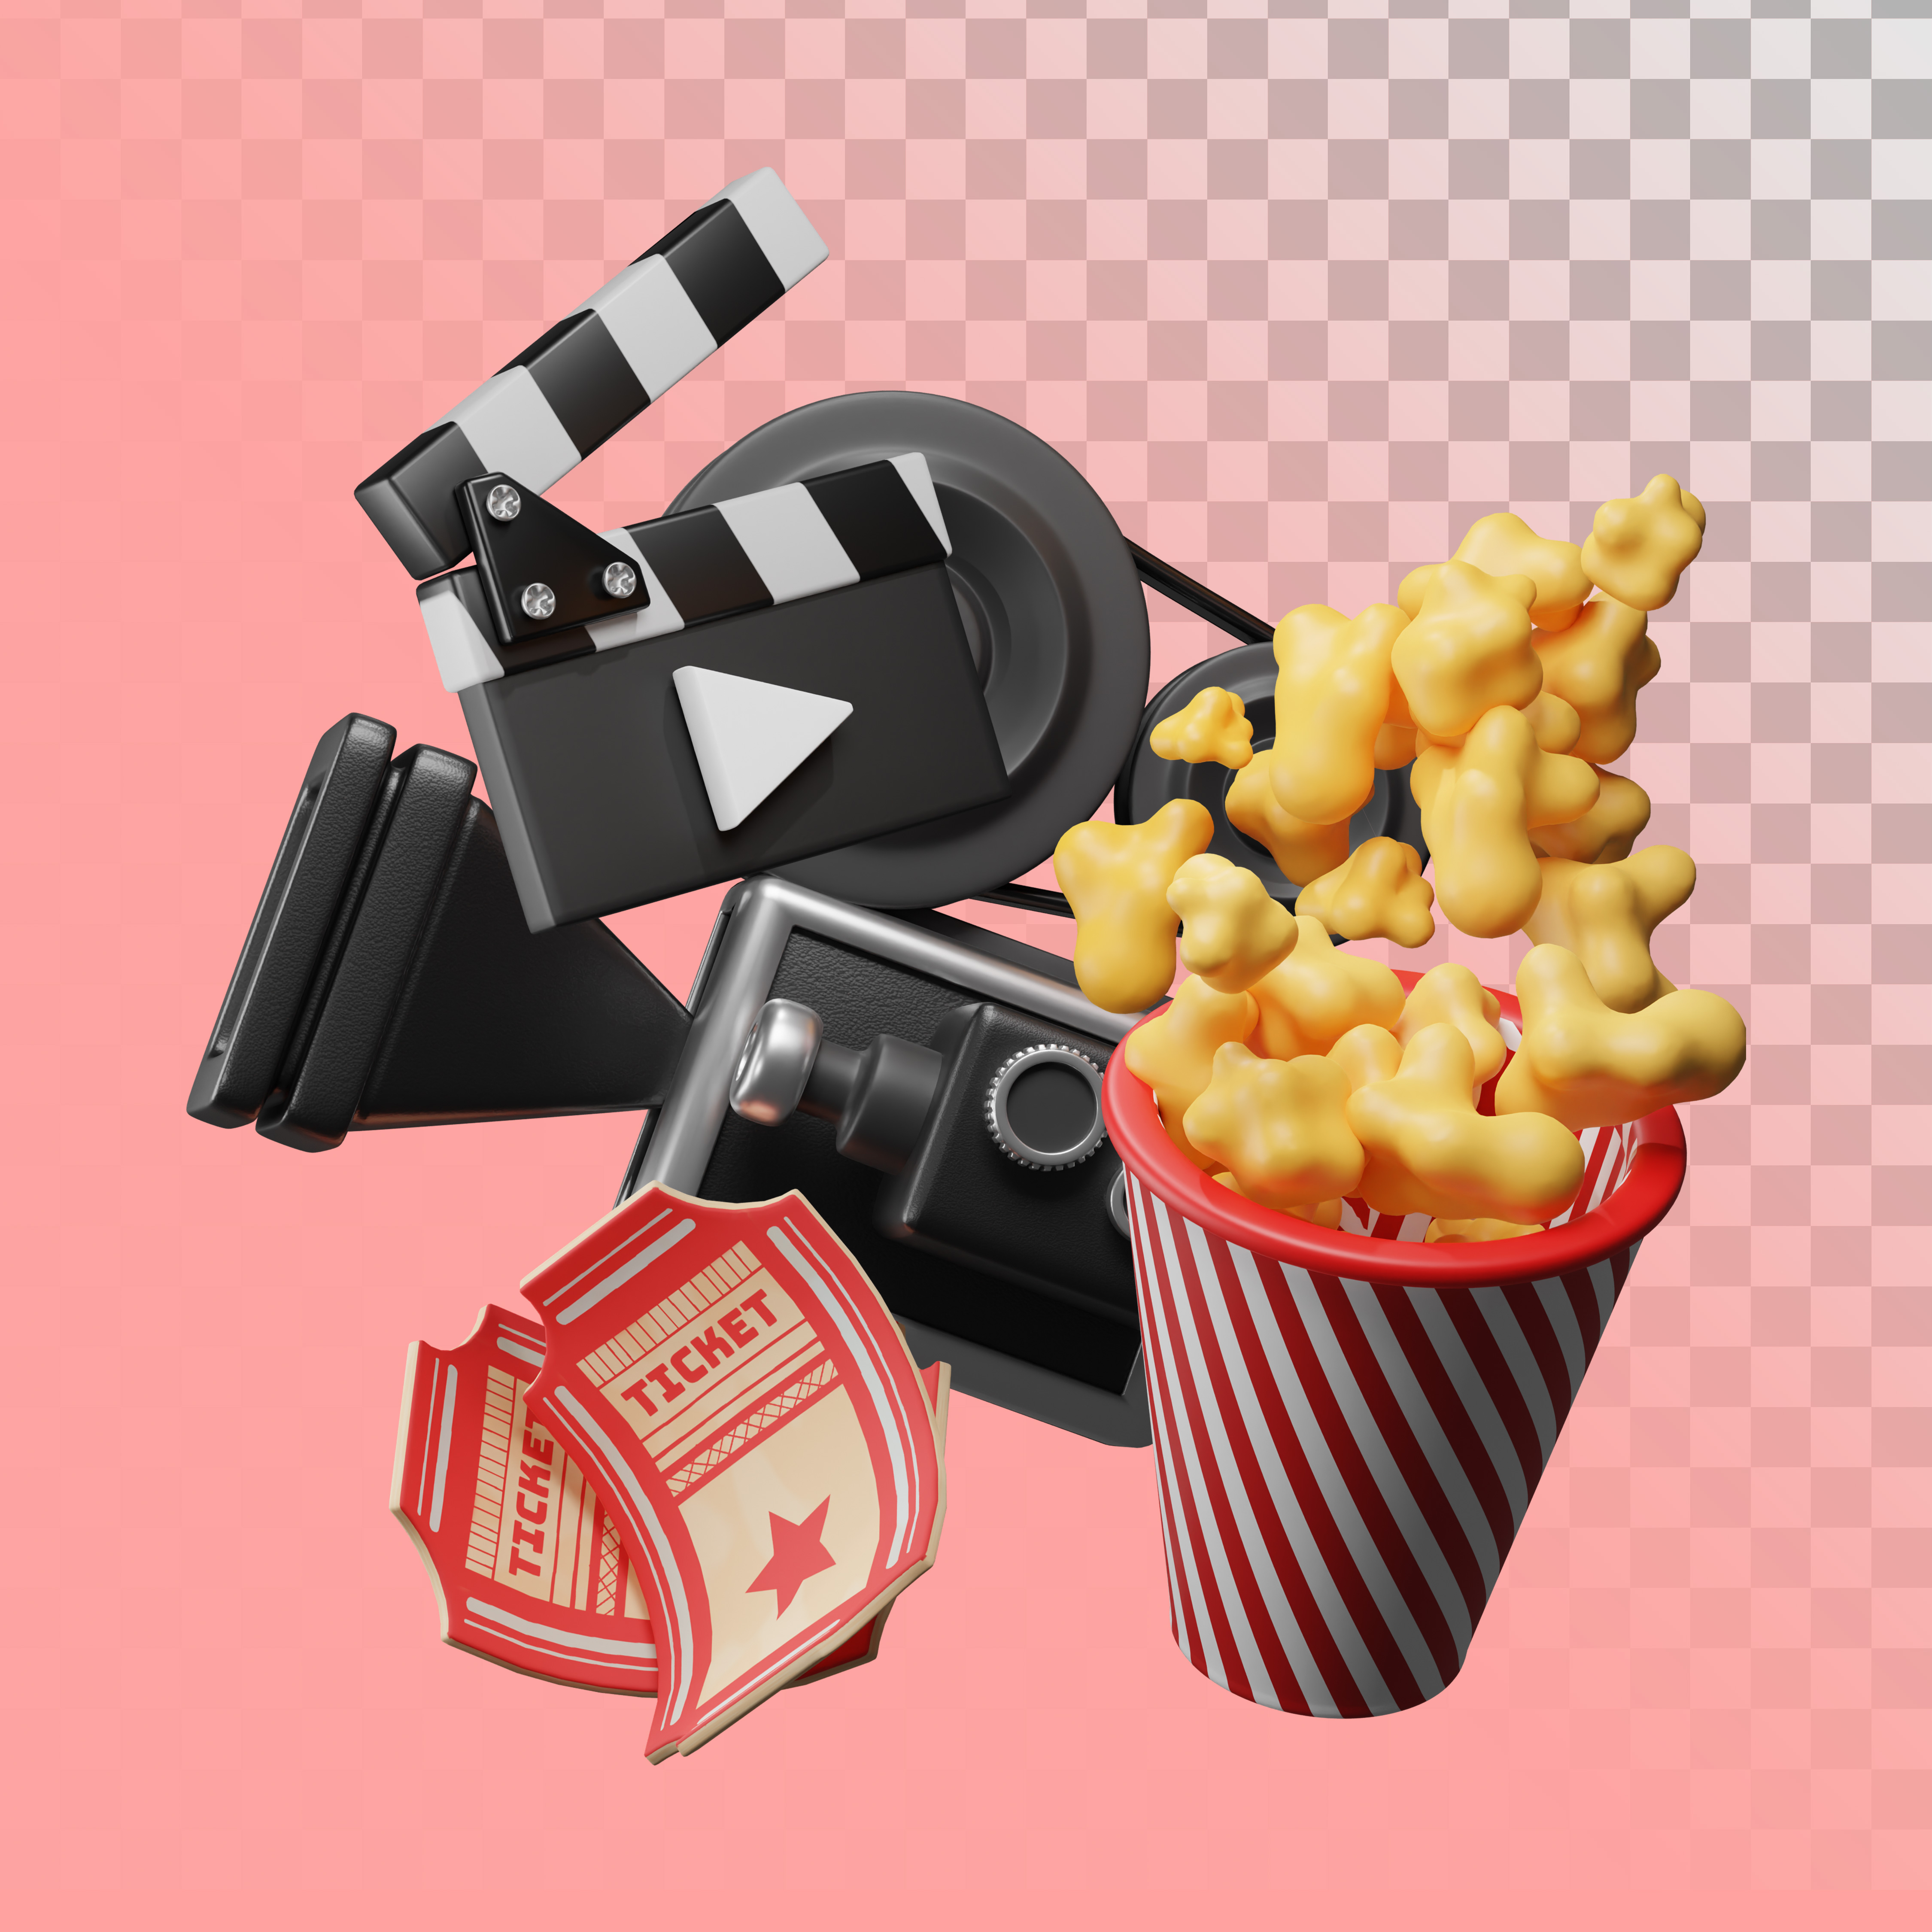
\includegraphics[width=0.7\textwidth]{./imgSAEB_6_POR/freepik/PORT_6_IMG-3.jpeg}
\end{figure}


\num{5} Assinale verdadeiro (V) ou falso (F) para as afirmações a
seguir.

\begin{boxlist}
\boxitem{F} A resenha tenta convencer o(a) leitor(a) a assistir ao filme.
\boxitem{V} O visual colorido do filme favorece a imaginação das pessoas que
assistem a ele.
\boxitem{V} A lição do filme é pontuar os laços de amizade, mesmo que em meio às
diferenças.
\boxitem{F} No filme, as personagens são apresentadas como ingênuas e até mesmo
bobas.
\boxitem{F} O diretor do filme, Daniel Rezende, pretende desvincular as
personagens de seu autor, Maurício de Sousa.
\boxitem{V} O filme apresenta crianças em situações de aventuras atemporais, sem
precisar de celulares e outros dispositivos eletrônicos para se
divertir.
\end{boxlist}

% Conforme explica o último parágrafo, o diretor resgata uma infância com
% sabor nostálgico de passado, sem a mediação de dispositivos eletrônicos.}

\num{6} De que maneira o(a) leitor(a) do texto percebe que o autor da
crítica gostou do filme?

\reduline{O autor da resenha utiliza adjetivos positivos sobre a obra,
ou seja, fala bem das cenas, do visual, do comportamento das personagens
e até mesmo do diretor do longa.\hfill}\linhas{1}

\num{7} Retire do texto ao menos dois trechos que demonstram o
posicionamento do autor da resenha em relação ao filme \emph{Turma da
Mônica: Laços}.

% Espera-se que os(as) estudantes retirem do texto trechos que apresentam adjetivos positivos em relação à obra. Sugestões de resposta:

\reduline{A ingenuidade delas tem seus limites e não é exagerada, o que retrata a
infância sem tornar os personagens bobos ou pouco realistas.\hfill}\linhas{1}

\reduline{Daniel Rezende, que já demonstrou suas habilidades como diretor em Bingo: O Rei das Manhãs (2017) presta uma preciosa homenagem à imaginação de Maurício de Sousa neste seu segundo longa-metragem.\hfill}\linhas{1}

\noindent\textbf{A crônica argumentativa é um gênero textual que busca
apresentar reflexões pontos de vista pessoais a respeito de temas ou
situações cotidianas. Leia a crônica \emph{A prisão Digital}, de Diva
Lopes, e responda às questões 8, 9 e 10.}


\begin{quote}
Era uma vez uma era digital, onde a tecnologia avançada tomou conta do
cotidiano das pessoas. Smartphones, tablets e computadores se tornaram
extensões de seus corpos, oferecendo uma miríade de possibilidades. Mas,
como tudo na vida, o encanto dessa modernidade tinha um preço oculto.

O vício em tecnologia se infiltrou nas vidas das pessoas
sorrateiramente, como uma teia virtual que as envolvia. O fascínio
inicial pela praticidade e pela conexão instantânea foi gradualmente
substituído por uma necessidade insaciável de estar online. A busca
frenética por \emph{likes}, seguidores e notificações se tornou o novo padrão
de validação social.

Nas mesas de jantar, as famílias se reuniam, mas os olhares se perdiam
nas telas iluminadas. A comunicação cara a cara foi substituída por
emojis e mensagens curtas. As ruas antes repletas de risos e conversas
agora se tornaram um desfile de cabeças baixas, imersas em um mundo
virtual que parecia mais real do que o próprio mundo real.

Os sinais de dependência eram claros. O sujeito se sentia ansioso quando
separado de seu dispositivo eletrônico, experimentando uma espécie de
abstinência tecnológica. Noites em claro eram gastas em redes sociais,
jogos online e maratonas intermináveis de séries, deixando de lado o
sono reparador e a vida social \emph{offline}.

A sociedade despertou para a realidade assustadora: a tecnologia que
inicialmente prometia facilitar a vida agora se tornara uma prisão
invisível. As pessoas eram escravas de suas próprias criações. Mas, como
em todas as histórias, havia uma oportunidade de mudança.

A conscientização sobre o vício em tecnologia começou a ganhar força.
Campanhas de desconexão foram lançadas, incentivando as pessoas a
encontrarem um equilíbrio saudável entre o mundo digital e o mundo real.
Pessoas corajosas começaram a se desconectar, a olhar nos olhos uns dos
outros e a redescobrir a beleza das conversas profundas e do toque
humano.

É verdade que a tecnologia trouxe avanços incríveis e facilitou muitos
aspectos de nossas vidas. No entanto, é fundamental reconhecer os
limites e controlar seu poder. Devemos lembrar que somos seres humanos,
dotados de emoções, relacionamentos e conexões reais. A tecnologia deve
ser uma ferramenta, não uma prisão que nos afasta da nossa essência.

Então, que possamos nos desconectar quando necessário, aproveitar
momentos de silêncio e introspecção, olhar para o céu, sentir a brisa e
abraçar aqueles que amamos. Que possamos encontrar o equilíbrio entre o
mundo digital e o mundo real, e assim viver uma vida plena, livre das
correntes invisíveis do vício em tecnologia.

\fonte{Diva Lopes. \emph{A prisão digital}.}
\end{quote}


\begin{figure}[H]
%PORT_6_IMG-4 — POR.tex:289
\centering\includegraphics[width=0.7\textwidth]{./imgSAEB_6_POR/freepik/PORT_6_IMG-4.jpeg}
\end{figure}


\num{8} No primeiro parágrafo, há um jogo de palavras logo no início, em
que duas palavras escritas de forma idêntica apresentam significados
diferentes. Quais são essas palavras e como os significados delas se
diferenciam?

\reduline{Trata-se das duas ocorrências da palavra ``era'' — a primeira é uma forma verbal e a segunda é o nome de um longo período de tempo.\hfill}\linhas{1}

\num{9} O que significa a palavra ``miríade'', utilizada no texto? Se
for preciso, faça uma pesquisa sobre ela. Como essa palavra contribui
para a construção da argumentação na crônica?

\reduline{A palavra significa ``um grande número ou quantidade indefinida de algo''. Na crônica, ela mostra a força do universo digital, que, por sua imensa quantidade de possibilidades, não só envolve como também vicia as pessoas.\hfill}\linhas{1}

\num{10} Qual é a mensagem final que se deixa no texto? Como você a
interpreta?

\reduline{A mensagem é que devemos nos reconectar ao mundo real, sabendo estar desconectados para aproveitar aquilo que só existe fora dos aparelhos e dos aplicativos.\hfill}\linhas{1}

\section{Treino}

\begin{figure}[H]
%PORT_6_IMG-5 — POR.tex:332
\centering\includegraphics[width=0.7\textwidth]{./imgSAEB_6_POR/freepik/PORT_6_IMG-5.jpeg}
\end{figure}

\begin{quote}
O consumismo está diretamente ligado à ideia de devorar, destruir e
extinguir. Se hoje testemunhamos tragédias naturais como queimadas,
furacões, inundações gigantescas e períodos prolongados de seca
ocorrendo com maior frequência, é porque a exploração irresponsável do
meio ambiente prevaleceu ao longo de décadas.

Focar todos os esforços no consumo é contribuir, dia após dia, para o
desequilíbrio global. O consumismo infantil, portanto, é um problema que
vai além da esfera educacional, seja na escola ou em casa. Embora seja
comumente associado à responsabilidade familiar, devemos compreender que
crianças que aprendem a consumir de forma inconsequente e desenvolvem
critérios e valores distorcidos representam um problema ético, econômico
e social.

\fonte{\emph{Consumismo infantil: um problema de todos}. Disponível em: https://criancaeconsumo.org.br/consumismo-infantil. Acesso em: 22 fev. 2022. Fragmento.}
\end{quote}

\num{1} Segundo o texto, o fato de o consumismo estar relacionado ao
desequilíbrio global é apoiado pelo argumento de que

\begin{escolha}
\item As crianças aprendem a consumir de forma inconsequente.
\item Critérios e valores distorcidos são passados para as pessoas desde a
infância.
\item A exploração irresponsável do meio ambiente prevaleceu ao longo de
décadas.
\item Critérios e valores distorcidos são problemas de ordem ética,
econômica e social.
\end{escolha}

% Gabarito, treino?
% A. Incorreta. O texto afirma que as crianças aprendem a consumir de forma inconsequente, porém não é essa a principal razão do desequilíbrio global.
% B. Incorreta. Critérios e valores distorcidos de consumo são passados para as pessoas desde a infância, e não critérios e valores distorcidos de modo geral, como dá a entender a afirmativa.
% C. Correta. O fato de explorarmos de forma irresponsável o meio ambiente ao longo de décadas é o principal responsável pelo desequilíbrio global.
% D. Incorreta. Critérios e valores distorcidos com relação ao consumo (e não de modo geral) são de fato problemas de ordem ética, econômica e social, porém não são os responsáveis diretos pelo desequilíbrio global.

%\paragraph{BNCC: EF67LP05}

\num{2} Observe a imagem e o texto a seguir.

\begin{figure}[H]
%PORT_6_IMG-6 — POR.tex:357
\centering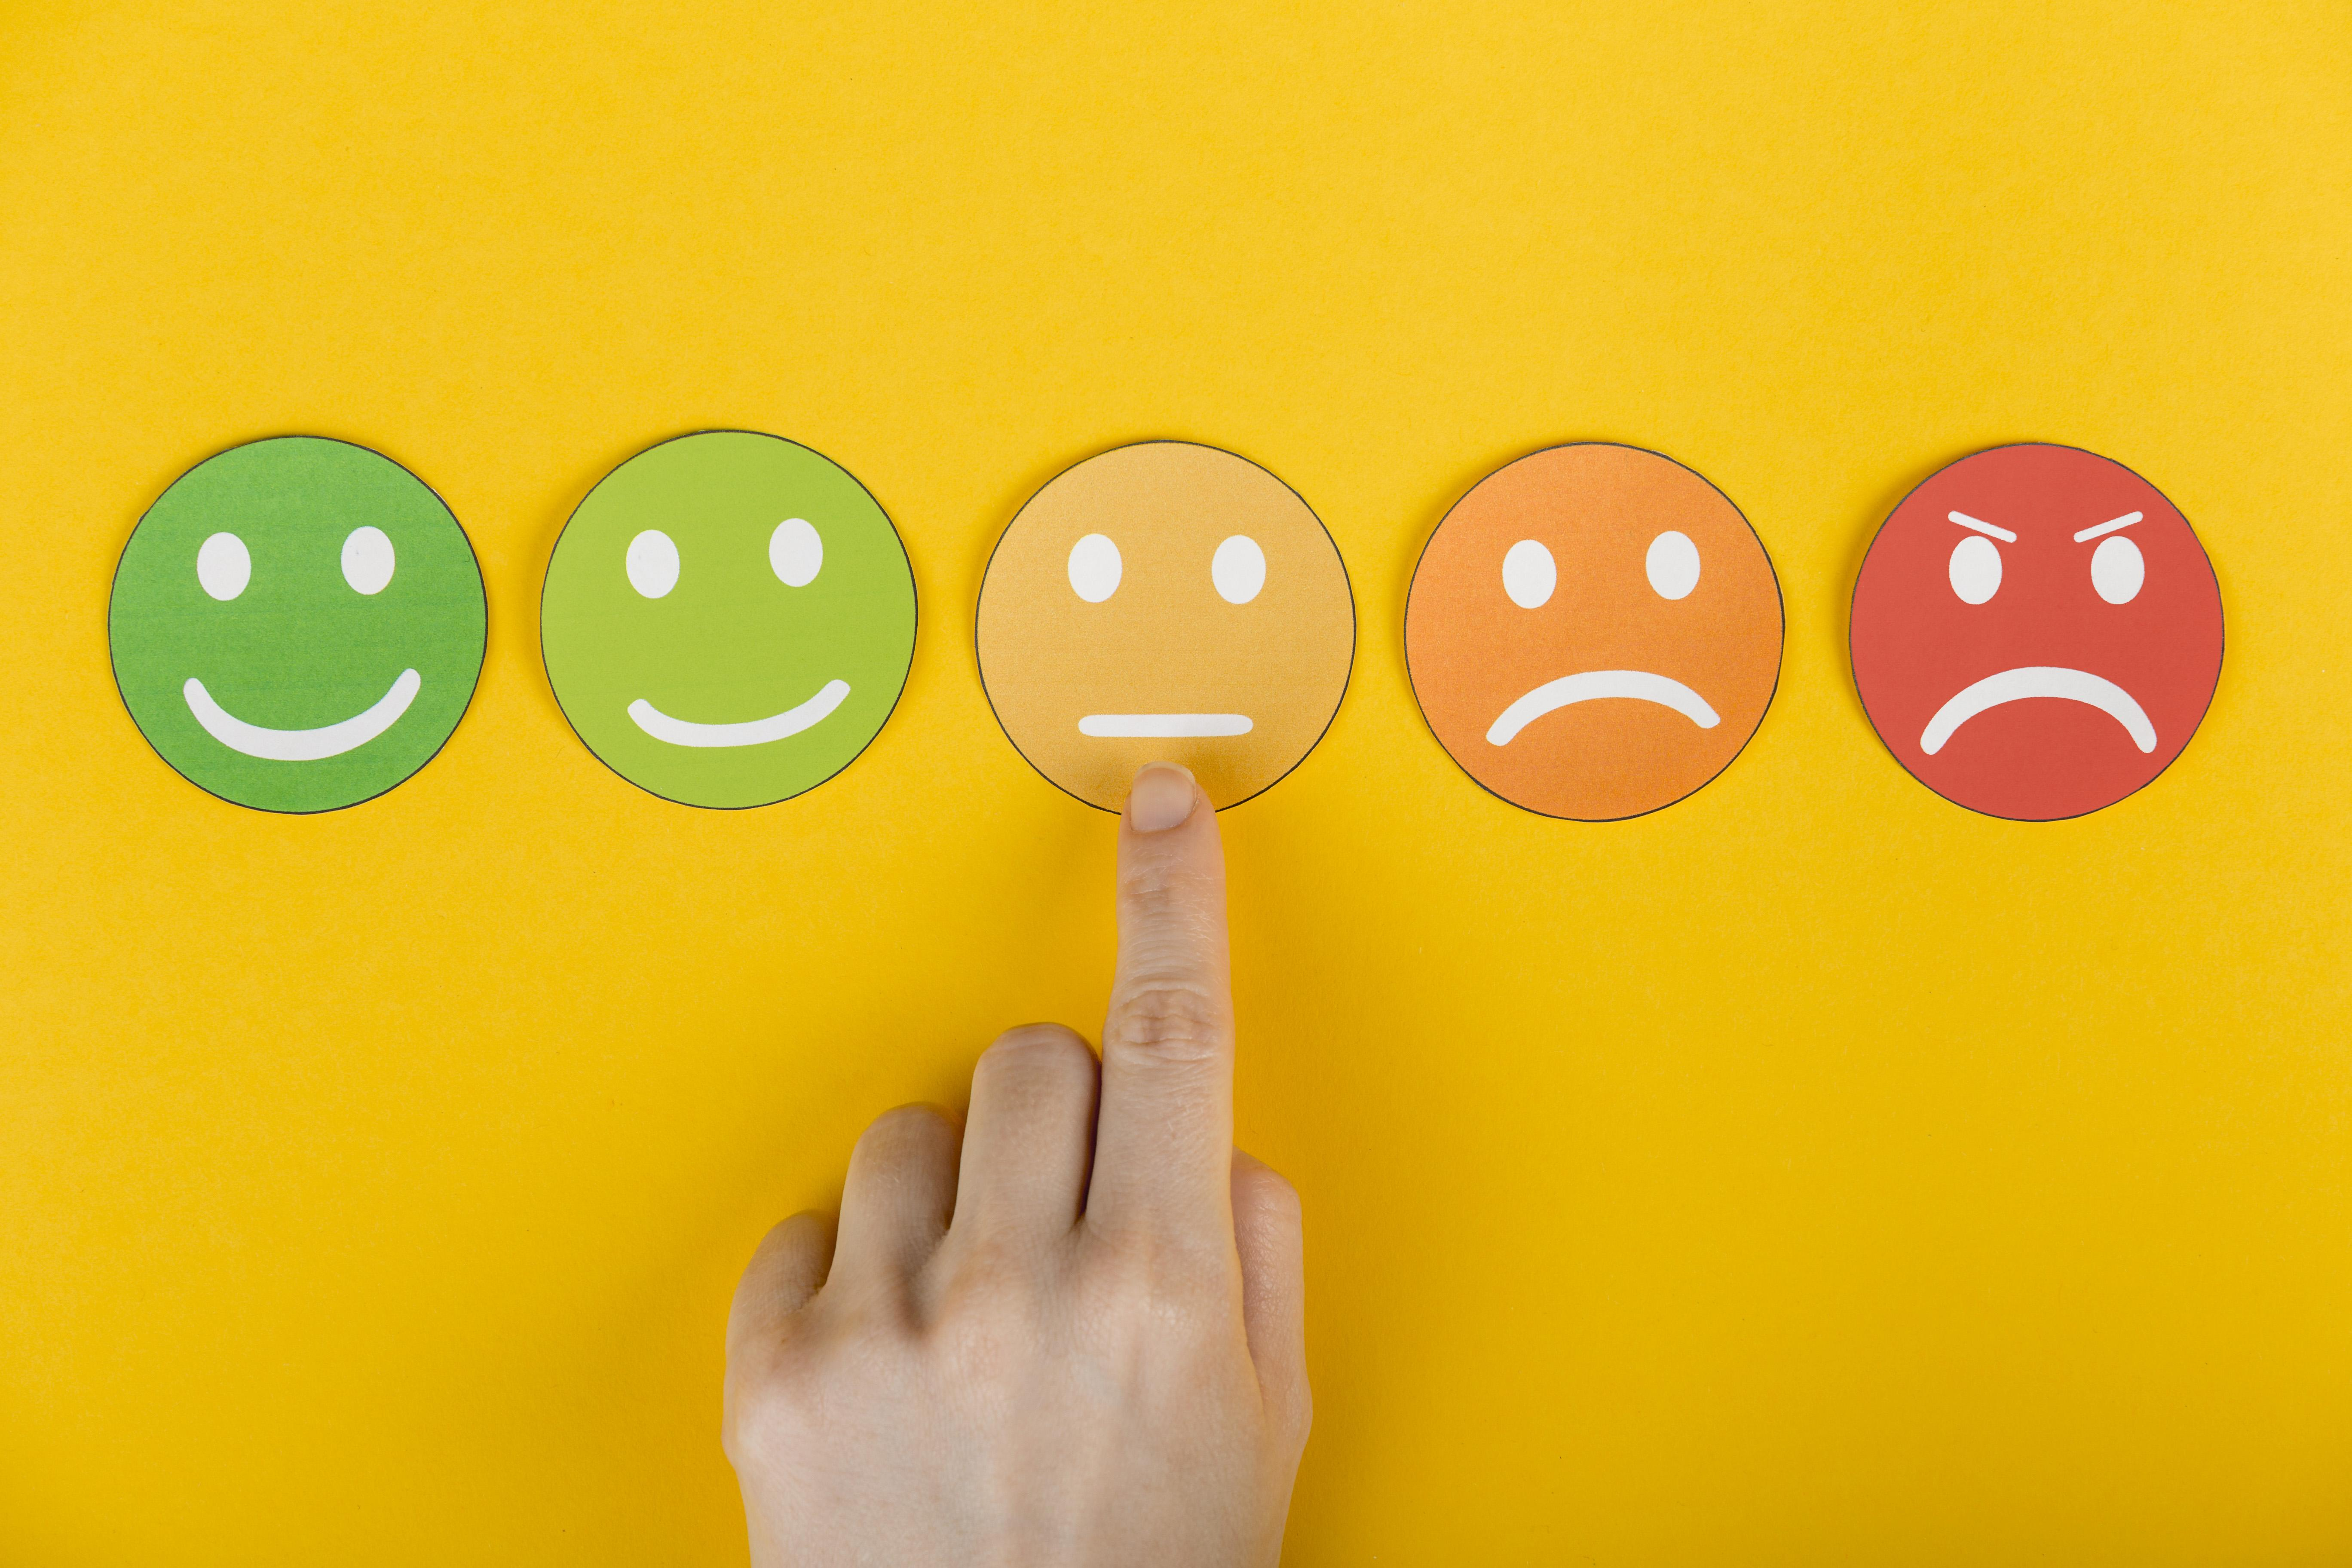
\includegraphics[width=0.7\textwidth]{./imgSAEB_6_POR/freepik/PORT_6_IMG-6.jpeg}
\end{figure}

\begin{quote}
``Quão satisfeito você está com nossos serviços? Muito insatisfeito,
Insatisfeito, Sem opinião definida, Satisfeito, Muito satisfeito.'' A imagem faz parte de uma pesquisa de satisfação. Os recursos que
auxiliam o(a) cliente a identificar com facilidade seu sentimento com
relação aos serviços nessa pesquisa são:
\end{quote}

\begin{escolha}
\item Os emojis, por estarem muito presentes no dia a dia das pessoas.
\item Os textos, que variam de ``muito insatisfeito'' a ``muito
satisfeito'', comumente posicionados abaixo das imagens.
\item As cores das imagens, que variam em uma escala de vermelho para
``muito insatisfeito'' a verde para ``muito satisfeito''.
\item A combinação de emojis com expressões faciais, as cores universais e
os textos abaixo das imagens, tornando a pesquisa inclusiva.
\end{escolha}

%\paragraph{BNCC: EF67LP07} % Identificar o uso de recursos persuasivos em textos
% argumentativos diversos (como a elaboração do título, escolhas lexicais,
% construções metafóricas, a explicitação ou a ocultação de fontes de
% informação) e perceber seus efeitos de sentido.

% Gabarito, treino?
% \begin{enumerate}
% \def\labelenumi{\alph{enumi})}
% \item Incorreta. Os emojis de fato estão presentes no dia a dia das pessoas
% que utilizam ferramentas de comunicação digital, por exemplo, mas
% aqueles que não estão familiarizados com esse tipo de linguagem poderiam
% se confundir.
% \item Incorreta. Os textos traduzem as expressões dos emojis, mas somente
% eles não tornam a pesquisa intuitiva.
% \item Incorreta. Os emojis estão representados em cores de sinalização
% praticamente universal, que já fazem parte do nosso cotidiano, como o
% semáforo: vermelho quando não se deve prosseguir, amarelo para alerta e
% verde para prosseguir. Contudo, sozinhas as cores não fazem sentido na
% pesquisa, elas precisam estar atreladas a uma imagem.
% \item Correta. A combinação de expressões faciais, texto de apoio e cores
% torna a pesquisa intuitiva, ou seja, fácil de ser respondida por todos
% os públicos, e inclusiva, isto é, acessível a todas as pessoas.
% \end{enumerate}

\num{3} \emph{``Nunca subestime uma mulherzinha''} é uma reunião de contos e
crônicas publicados pela autora nos jornais~\emph{Correio
Braziliense}~e~\emph{O Estado de Minas}, com prefácio de~Zélia Duncan. 

\begin{quote}
Neste texto, os leitores poderão testemunhar o talento literário e a
irreverência de Fernanda Takai, uma mulher de estatura pequena, com
pouco mais de um metro e meio, e uma voz suave. Em sua trajetória no
Pato Fu, ela costumava se esconder atrás de uma guitarra.

\fonte{Disponível em: https://fernandatakai.com.br/livros. Acesso em: 22 de fev. 2023.}
\end{quote}

\begin{figure}[H]
%PORT_6_IMG-7 — POR.tex:408
\centering
\includegraphics[width=\textwidth]{./imgSAEB_6_POR/freepik/PORT_6_IMG-7.jpeg}
\end{figure}

\noindent No título do livro de Fernanda Takai, \emph{Nunca subestime uma
mulherzinha}, a palavra ``mulherzinha'', no diminutivo, foi escolhida no
intuito de

\begin{escolha}
\item Fazer uma chacota com o fato de a autora ser uma mulher baixinha.
\item Tratar mulheres pequenas como autoras de forma carinhosa, ou seja,
``mulherzinhas''.
\item Brincar com o fato de a autora ser uma mulher tão pequena que se
escondia atrás da guitarra.
\item Dar um novo sentido à palavra ``mulherzinha'', que pode ser
pejorativo em alguns contextos, mas aqui está sendo usado para
representar a autora, uma mulher baixinha.
\end{escolha}

%\paragraph{BNCC: EF67LP07} 
% Identificar o uso de recursos persuasivos em textos
% argumentativos diversos (como a elaboração do título, escolhas lexicais,
% construções metafóricas, a explicitação ou a ocultação de fontes de
% informação) e perceber seus efeitos de sentido.

% Gabarito, treino?
% \begin{enumerate}
% 	\def\labelenumi{\alph{enumi})}
% \item Incorreta. A intenção de usar a palavra ``mulher'' no diminutivo não
% é fazer chacota com a autora do livro: pelo contrário, é ironizar o fato
% de mulheres serem subestimadas por supostamente não conseguirem fazer
% certas coisas.
% \item Incorreta. Algumas vezes o diminutivo é usado de forma carinhosa,
% porém, neste caso, a palavra ``mulherzinha'' é usada de forma irônica.
% \item Incorreta. A palavra no diminutivo de certa forma brinca com o fato
% de a autora ser uma mulher pequena, porém ela tem outro efeito de
% sentido além desse.
% \item Correta. Chamar uma mulher de ``mulherzinha'' em alguns contextos é
% pejorativo, contudo, neste caso, pretende-se dar outro efeito de sentido
% à palavra ironizando esse fato ao mesmo tempo em que a palavra é usada
% em sentido literal, para representar a autora, que é uma mulher
% realmente pequena.
% \end{enumerate}

\chapter{Eu, a sociedade, direitos e deveres}
\markboth{Módulo 2}{}

\section{Habilidades do SAEB}
\begin{itemize}
\item Identificar elementos constitutivos de textos pertencentes ao domínio jornalístico/midiático.
\item Identificar formas de organização de textos normativos, legais e/\,ou reinvindicatórios.
\item Identificar elementos constitutivos de gêneros de divulgação científica.
\item Analisar a relação temática entre diferentes gêneros jornalísticos.
\end{itemize}

\subsection{Habilidades da BNCC} 
\begin{itemize}
\item EF69LP02
\item EF69LP20
\item EF69LP27
\item EF67LP16
\item EF67LP17
\end{itemize}

\conteudo{Os \textbf{textos expositivos} são aqueles que têm como objetivo expor
informações, apresentando ao leitor determinado assunto. Com uma
linguagem clara e objetiva, esse tipo de texto apresenta uma ideia
central que, em alguns casos, é o fio condutor para que um autor
argumente sobre ela.

Os textos expositivos podem ser de dois tipos diferentes:
\begin{itemize}
\item Expositivos informativos, cuja função é apenas informar sobre
  determinado assunto, sem que o autor coloque seu ponto de vista
  pessoal com relação a ele. Exemplos: artigo de divulgação científica,
  livros didáticos, enciclopédias, verbetes de dicionários, textos
  acadêmicos, textos normativos, como leis, e infográficos.
\item Expositivos argumentativos, no qual o autor geralmente apresenta seu
  ponto de vista sobre o tema, embasando-se em uma série de estratégias
  argumentativas. Exemplos: carta de reclamação, artigo de opinião,
  textos enviados em páginas de internet voltadas ao atendimento ao
  cliente, comentários em redes sociais, entre outros.
\end{itemize}

Os textos expositivos estão mais presentes em nosso dia a dia do que
imaginamos, e podem utilizar \textbf{recursos verbais e não verbais}.
Por exemplo, ao atravessar a rua distraído, você provavelmente ouviu
algum veículo buzinar para chamar sua atenção com relação ao perigo,
certo? Ainda com relação ao trânsito, o próprio semáforo é um tipo de
texto informativo, pois mesmo que as informações não sejam transmitidas
com palavras, a sequência de cores e luzes aciona em nós os comandos de
``pare'', ``atenção'' e ``siga em frente''.

É importante lembrar que sempre que vamos argumentar, ou seja, defender
um ponto de vista, é preciso utilizar estratégias corretas e voltadas a
cada tipo de texto.

Confira a seguir as principais estratégias argumentativas que podemos
utilizar em textos expositivos.}

\conteudo{
\paragraph{Dados estatísticos de fontes confiáveis} Esse tipo de informação, quando extraída de fontes confiáveis, parte de pesquisas desenvolvidas por especialistas em diversas áreas do conhecimento, o que as torna praticamente irrefutáveis, ou seja, incontestáveis. Exemplo: \emph{De acordo com uma pesquisa do Ministério da Saúde}, as crianças estão mais vulneráveis a sofrer problemas respiratórios no inverno.

\paragraph{Exemplificação} Vivências comuns ao dia a dia das pessoas possibilitam o contato com situações que podem ser usadas para exemplificar seus argumentos. Exemplo: A falta de oportunidades profissionais para pessoas com pouca experiência muitas vezes faz com que jovens se vejam obrigados a trabalhar em profissões que não condizem com sua área de formação, \emph{a exemplo} dos motoristas de aplicativo.

\paragraph{Comparação} Utilizar séries, documentários, novelas, personagens, pessoas de referência e outros repertórios que fazem parte da sua vivência podem embasar um argumento e gerar uma aproximação do leitor com o texto.\\ Exemplo: \emph{Assim como} a apresentadora Xuxa, é importante que outras celebridades se posicionem a respeito da importância de uma alimentação saudável, pois isso serve de inspiração para que mais pessoas adotem estilos de vida semelhantes.

\paragraph{Causa e consequência} Para buscar a solução de um problema, é preciso identificar sua causa. Quais são as consequências do problema para as pessoas? Como ele surgiu? Exemplo: \emph{Desde a colonização, a população indígena foi escravizada e colocada à margem nossa sociedade. Uma das consequências disso} é o desrespeito, até os dias de hoje, às terras demarcadas e garantidas aos povos nativos.

\paragraph{Citação} Quando se tem uma opinião sólida e declarada, (como em uma entrevista), de um(a) especialista no assunto. Exemplo: \emph{De acordo com o médico} Dráuzio Varella, fumar é um hábito prejudicial à saúde de modo geral.
}


\section{Atividades}

\noindent Leia o texto a seguir, publicado no Jornal da USP, e responda às
questões de 1 a 3.

\begin{figure}[H]
%PORT_6_IMG-8 — POR.tex:564
\centering
\includegraphics[width=\textwidth]{./imgSAEB_6_POR/freepik/PORT_6_IMG-8.jpeg}
\end{figure}


\begin{quote}
\centering\noindent\textbf{Seu cão reconhece suas emoções e toma decisões a partir disso, mostra estudo da USP}

\noindent \small{\emph{Pesquisa do Instituto de Psicologia mostra que ``nossos melhores
amigos'' podem prever o comportamento humano ao olhar para nosso rosto e
diferenciar emoções neutras, de alegria ou raiva.}}
\medskip

\noindent Será que seu cachorro sabe o que fazer quando você está bravo ou feliz?
Com o objetivo de entender se os cães respondem de forma diferente às
expressões humanas positivas e negativas, pesquisadores do Instituto de
Psicologia (IP) da USP e da Universidade de Lincoln, no Reino Unido,
estudaram 90 cães e descobriram que eles são capazes não apenas de
inferir emoções humanas através de expressões faciais, mas também de
relacionar essa informação com suas possíveis consequências e tomar
decisões a partir de uma previsão do nosso comportamento.

O artigo intitulado \emph{Dogs can infer implicit information from human
emotional expressions}
% \footnote{\emph{Dogs can infer implicit information from human emotional
%  expressions}, em português significa ``Cães podem inferir informações
%  implícitas em expressões humanas relacionadas a emoções''.} 
foi publicado na
 revista científica \emph{Animal Cognition} e desenvolvido pelos
 pesquisadores Natalia Albuquerque e Briseida Resende, do Instituto de
 Psicologia da USP, e Daniel Mills, Kun Guo e Anna Wilkinson, da Universidade
 de Lincoln.{[}\ldots{}{]}

``A pesquisa evidencia que os cães levam em conta as expressões das
emoções dos humanos para fazer escolhas. As pessoas poderão perceber o
animal como um ser que presta atenção ao que fazemos e que toma suas
decisões com base nisso. Desta forma, acho que podemos desenvolver uma
relação mais saudável e respeitosa'', afirma a coautora do trabalho, a
professora Briseida. Ela destaca que é importante não o tratar como
humano, e sim respeitá-lo enquanto cão.

\fonte{Guilherme Gama. Jornal da USP. Seu cão reconhece suas emoções e toma decisões a partir disso, mostra 
estudo da USP. Disponível em: https://jornal.usp.br/ciencias/
seu-cao-reconhece-suas-emocoes-e-toma-decisoes-a-partir-disso-mostra-estudo-da-usp. Acesso em: 01 mar. 2023. (
Adaptado.)}

\end{quote}

\num{1} Qual é o principal assunto do texto? Em que parte da estrutura
do texto é possível constatar essa informação?

\reduline{O texto fala sobre a capacidade dos cães de reconhecerem as
emoções humanas e tomarem decisões a partir disso. É possível constatar
essa informação no título do texto.\hfill}\linhas{1}

\num{2} Qual é a função do subtítulo do artigo?

\reduline{O subtítulo apresenta para o leitor a pesquisa que será
apresentada no artigo.\hfill}\linhas{1}

\num{3} Qual é o objetivo de se fazer a pesquisa apresentada no artigo?
Em que parte do texto é possível obter essa informação?

\reduline{O objetivo, segundo a pesquisadora, é desenvolver uma relação
mais saudável e respeitosa entre pessoas e animais, a partir das
informações constatadas. Essa informação encontra-se no último parágrafo
do texto.\hfill}
\linhas{6}

\pagebreak

\noindent Observe com atenção os textos I e II, a seguir, para responder às
questões 4 a 6.

\begin{quote}

\begin{figure}[h!]
%PORT_6_IMG-9 — POR.tex:638
\centering\includegraphics[width=0.7\textwidth]{./imgSAEB_6_POR/freepik/PORT_6_IMG-9.jpeg}
\end{figure}
Precisamos prevenir a obesidade infantil, para não precisarmos lidar com a doença nos adultos depois.

\begin{figure}[h!]
%PORT_6_IMG-10 — POR.tex:645
\centering\includegraphics[width=0.7\textwidth]{./imgSAEB_6_POR/freepik/PORT_6_IMG-10.jpeg}
\end{figure}

Hábitos saudáveis começam na infância. \#obesidadeinfantilnão
\end{quote}



\num{4} O objetivo comum a ambas as campanhas é

\begin{escolha}
\item Mostrar às crianças como cuidar da saúde.
\item Incentivar as pessoas a manterem hábitos saudáveis na infância.
\item Apresentar o que deve ser feito para que crianças não sofram
obesidade.
\item Conscientizar as pessoas com relação ao problema da obesidade
infantil. 
\end{escolha}

% \coment{Resposta: D. Ambos os textos são campanhas de
% conscientização com relação à obesidade infantil.

\num{5} Como a presença da hashtag \#obesidadeinfantilnão ajuda no
envolvimento do público na campanha?

\reduline{A hashtag moderniza e atualiza o texto, mostrando às pessoas que a saúde desde a infância é uma responsabilidade de todos.\hfill}\linhas{1}

\num{6} Onde você imagina que a segunda campanha pode ter circulado? Por
quê?

\reduline{A segunda campanha provavelmente circulou em uma rede social, o que é indicado pela presença da hashtag.\hfill}\linhas{1}

\noindent Leia, a seguir, o artigo 4º da Declaração Universal dos Direitos dos
Animais e responda às questões 7 e 8.

\begin{enumerate}
\item Todo o animal pertencente a uma espécie selvagem tem o direito de
viver livre no seu próprio ambiente natural, terrestre, aéreo ou
aquático e tem o direito de se reproduzir.
\item Toda a privação de liberdade, mesmo que tenha fins educativos, é
contrária a este direito.
\end{enumerate}

\fonte{Disponível em: http://www.fiocruz.br/biosseguranca/Bis/infantil/direitoanimais.htm. Acesso em: 2 mar. 2023. Fragmento.}

\begin{figure}[H]
%PORT_6_IMG-11 — POR.tex:683
\centering\includegraphics[width=0.7\textwidth]{./imgSAEB_6_POR/freepik/PORT_6_IMG-11.jpeg}
\end{figure}

\num{7} Explique, com suas palavras e com base na leitura, a finalidade
da Declaração Universal dos Direitos dos Animais.

\reduline{A Declaração Universal dos Direitos dos Animais tem a
finalidade de garantir que os direitos dos animais sejam preservados por
nós, seres humanos.\hfill}

\num{8} O parágrafo 2 da Declaração Universal dos Direitos dos Animais
informa que toda a privação de liberdade no caso de animais selvagens,
mesmo que com fins educativos, é contrária a esse direito. Esse trecho
quer dizer que

\begin{escolha}
\item Prender animais selvagens é crime.
\item Não se podem prender animais selvagens, mas animais domésticos, sim.
\item É um dever dos seres humanos garantir o direito de animais selvagens
viverem em liberdade. 
\item Pessoas que estudam animais selvagens e restringem sua liberdade para
este fim estão, na realidade, cometendo um crime.
\end{escolha}

% \coment{ É um dever dos seres humanos garantir o direito de animais
% selvagens viverem em liberdade.

% Gabarito, treino?
% \begin{escolha}
% \item Incorreta. O texto orienta sobre direitos de animais selvagens,
% mas não informa que prendê-los é crime.
% \item Incorreta. O trecho não menciona nada sobre poder manter animais
% domésticos presos.
% \item Correta. A Declaração Universal dos Direitos dos Animais é um texto normativo que
% tem como princípio garantir direitos de sobrevivência dos animais de
% modo geral, a fim de orientar a convivência harmoniosa entre eles e os
% seres humanos. Cabe a nós garantir esse direito, uma vez que os animais
% são seres irracionais.
% \item Incorreta. O trecho menciona que restringir a liberdade de animais
% selvagens, mesmo que para estudo, fere esse direito, porém não menciona
% que é crime ou que a pessoa será punida por fazer isso.
% \end{escolha}

\num{9} Observe a imagem a seguir e leia o texto que a acompanha.

\begin{figure}[H]
%PORT_6_IMG-12 — POR.tex:732
\centering
\includegraphics[width=0.7\textwidth]{./imgSAEB_6_POR/freepik/PORT_6_IMG-12.jpeg}
\end{figure}

\begin{quote}
\centering\textsc{Símbolo do autismo passa a ser obrigatório em placas de atendimento
preferencial.}
\end{quote}

\noindent Por sua natureza reivindicatória, o objetivo do texto apresentado é
tornar o convívio entre as pessoas mais

\begin{escolha}
\item alegre.
\item bonito.
\item seguro.
\item justo.
\end{escolha}

% Gabarito, treino?
% \coment{\begin{enumerate}\def\labelenumi{\alph{enumi})}
% \item Incorreta. Não se trata de tornar o convívio mais alegre, e sim
% igualitário e inclusivo.
% \item Incorreta. O objetivo do texto normativo é regulamentar normas de
% bom convívio, a fim de tornar o dia a dia das pessoas mais justos em
% direitos.
% \item Incorreta. O direito a atendimento prioritário não faz da vida de
% pessoas pertencentes aos grupos da imagem mais segura.
% \item Mais justo. O texto normativo apresentado trata do direito ao atendimento
% prioritário dos grupos descritos nas imagens: idosos, gestantes, pessoas
% com crianças de colo, pessoas com deficiência e autistas. Por seu
% caráter reivindicatório, o objetivo é tornar o convívio entre as pessoas
% mais justo.
% \end{enumerate}}

\num{10} Observe o texto presente em uma rede social da prefeitura de
uma grande cidade.

\begin{figure}[H]
%PORT_6_IMG-13 — POR.tex:764
\centering
\includegraphics[width=0.7\textwidth]{./imgSAEB_6_POR/freepik/PORT_6_IMG-13.jpeg}
\end{figure}

\begin{quote}
\centering{Esses ônibus que passam aqui na Zona Sul depois das 18h estão
impossíveis. A linha 2345T é a pior de todas. É melhor andar a pé do que
pegar esses ônibus.}
\end{quote}


Atualmente, é muito comum as pessoas utilizarem plataformas digitais e
redes sociais para expor algum problema de impacto social, como esse da
imagem. O comentário do usuário, nesse caso, aproxima-se daquele
normalmente presente em:

\begin{escolha}
\item Um artigo de opinião.
\item Uma carta de reclamação.
\item Um texto informativo.
\item Uma campanha publicitária.
\end{escolha}

% Gabarito, treino?
% \coment{
% \begin{enumerate}
% \def\labelenumi{\alph{enumi})}
% \item Incorreta. O artigo de opinião é um gênero textual jornalístico que
% tem como objetivo comentar e opinar a respeito de um tema.
% \item Correta. A carta de reclamação é um gênero textual que expressa uma indignação ou
% uma insatisfação de determinado indivíduo diante de alguma relação
% comercial, de serviço ou compra, por exemplo. Na postagem, o consumidor
% reclama de ônibus de determinada linha, afirmando que é impossível
% viajar neles.
% \item Incorreta. O texto informativo tem como objetivo informar o(a)
% leitor(a) sobre determinado assunto, elucidando e esclarecendo-o(a)
% sobre o tema em questão.
% \item Incorreta. A campanha publicitária tem como objetivo persuadir uma
% pessoa a comprar um produto ou adotar um comportamento.
% \end{enumerate}}

\section{Treino}

\num{1} Leia o texto a seguir.

\textbf{O Brasil precisa do SUS: lançada campanha nacional de defesa do
Sistema Único de Saúde}

\begin{figure}[H]
%PORT_6_IMG-14 — POR.tex:804
\centering\includegraphics[width=0.7\textwidth]{./imgSAEB_6_POR/freepik/PORT_6_IMG-14.jpeg}
\end{figure}

\begin{quote}
A coordenadora do Campus Virtual Fiocruz, Ana Furniel, está alinhada com
a campanha \#OBrasilPrecisadoSUS, destacando a indispensabilidade do
Sistema Único de Saúde para o país. O papel desempenhado pelo SUS
durante a pandemia ressaltou ainda mais sua importância. ``É importante
pensar em sua totalidade, pois ao falarmos do SUS, ainda há uma
limitação em pensar apenas no atendimento hospitalar. No entanto, o SUS
vai além, abrangendo vacinas, medicamentos, atenção primária, vigilância
e, especialmente para nós, a formação de profissionais de saúde. Essa é
a área em que o CVF contribui.''

\fonte{Isabela Schincariol. Fiocruz. \emph{O Brasil precisa do SUS: lançada campanha nacional de defesa do Sistema Único de Saúde}. Disponível em: https://campusvirtual.fiocruz.br/portal/?q=noticia/59976. Acesso em: mar. 2023. Adaptado.}
\end{quote}

A hashtag indicada na campanha (\#OBrasilPrecisadoSUS) é, na realidade,

\begin{escolha}
\item Um incentivo para que pessoas reivindiquem a favor do SUS.
\item Um convite para que as pessoas utilizem os serviços do SUS.
\item Uma reivindicação para que o SUS seja defendido e não atacado.
\item Uma propaganda para divulgar nas redes sociais os serviços do SUS.
\end{escolha}

%\paragraph{BNCC: EF67LP16} 
% Explorar e analisar espaços de reclamação de direitos e de envio de solicitações (tais como ouvidorias, SAC, canais ligados a órgãos públicos, plataformas do consumidor, plataformas de reclamação), bem como de textos pertencentes a gêneros que circulam nesses espaços, reclamação ou carta de reclamação, solicitação ou carta de solicitação, como forma de ampliar as possibilidades de produção desses textos em casos que remetam a reivindicações que envolvam a escola, a comunidade ou algum de seus membros como forma de se engajar na busca de solução de problemas pessoais, dos outros e coletivos.

% Gabarito, treino?
% \begin{enumerate}
% \def\labelenumi{\alph{enumi})}
% \item Correta. A campanha é um incentivo para que as pessoas se
% conscientizem e reivindiquem a manutenção do SUS.
% \item Incorreta. A campanha não pretende convidar pessoas a utilizarem o
% SUS.
% \item Incorreta. A campanha, embora defenda o SUS, não informa que de
% alguma forma ele é atacado.
% \item Incorreta. Embora veiculada em redes sociais, a campanha busca
% defender a manutenção do SUS e não divulgar seus serviços.
% \end{enumerate}

\pagebreak

\num{2} O piso tátil, instalado em calçadas e estabelecimentos,
apresenta dois tipos de padrão: em bolinhas ou em faixas paralelas.

\begin{figure}[H]
%PORT_6_IMG-15 — POR.tex:857
\centering\includegraphics[width=0.7\textwidth]{./imgSAEB_6_POR/freepik/PORT_6_IMG-15.jpeg}
\end{figure}

\noindent Considerando-se seu uso, pode-se afirmar que o piso tátil

\begin{escolha}
\item Pretende sempre evitar que a pessoa cega acesse um objeto.
\item Pretende orientar a pessoa com deficiência visual por meio de sinais
e significados diversos.
\item Tem por objetivo direcionar a pessoa com deficiência visual para que
acesse determinado objeto; tendo as linhas e as bolinhas o mesmo
significado.
\item Deve proteger o chão da calçada de qualquer avaria em decorrência da
aproximação de pessoas com bengalas, por exemplo.
\end{escolha}

%\paragraph{BNCC: EF69LP20} 
% Identificar, tendo em vista o contexto de produção, a forma de organização dos textos normativos e legais, a lógica de hierarquização de seus itens e subitens e suas partes: parte inicial (título — nome e data — e ementa), blocos de artigos (parte, livro, capítulo, seção, subseção), artigos (caput e parágrafos e incisos) e parte final (disposições pertinentes à sua implementação) e analisar efeitos de sentido causados pelo uso de vocabulário técnico, pelo uso do imperativo, de palavras e expressões que indicam circunstâncias, como advérbios e locuções adverbiais, de palavras que indicam generalidade, como alguns pronomes indefinidos, de forma a poder compreender o caráter imperativo, coercitivo e generalista das leis e de outras formas de regulamentação.

% Gabarito, treino?
% \begin{enumerate}
% \def\labelenumi{\alph{enumi})}
% \item Incorreta. Nenhum piso tátil tem função de evitar que qualquer pessoa
% deixe de acessar um recurso público.
% \item Correta. O piso tátil em bolinha, conforme explica a imagem 1, é um
% alerta para a pessoa com deficiência visual, ou sejam, serve para
% orientá-la de que ali há um objeto; o piso com função de direcionamento
% é aquele com padrão em faixas; cada símbolo tem um significado
% diferente.
% \item Incorreta. formas diferentes, significados diferentes.
% \item Incorreta. A proteção é à pessoa, não ao ambiente público.
% \end{enumerate}

\num{3} Leia o texto a seguir.

\begin{quote}
Em 26 de janeiro de 2023, um asteroide com tamanho estimado semelhante
ao de um ônibus cruzou o céu do extremo sul da América do Sul pouco
depois das 21h (horário de Brasília). O objeto espacial, identificado
como 2023 BU, passou a uma distância aproximada de 3.600 km do nosso
planeta, o que é considerado uma proximidade significativa.

Apesar disso, não houve razão para alarme, apenas confirmou-se a
existência de asteroides de tamanho considerável que se aproximam
consideravelmente da Terra e necessitam ser rastreados.

Desta vez, não estivemos em perigo iminente; no entanto, os cientistas
estão continuamente empenhados em localizar asteroides que, em caso de
colisão com a Terra, poderiam causar danos consideráveis. Os verdadeiros
gigantes que estão presentes, como o asteroide de 12 km de diâmetro que
causou a extinção dos dinossauros, provavelmente já foram identificados
e não representam motivo de preocupação.

\fonte{O Globo. \emph{Asteroide do tamanho de ônibus deve passar
rente à América do Sul com a menor distância já registrada da Terra}. Disponível em: 
https://oglobo.globo.com/mundo/epoca/noticia/2023/01/asteroide-e-esperado-para-passar-rente-a-america-do-sul-com-a-menor-distancia-ja-registrada-da-terra.ghtml. Acesso em: 13 mai. 2023.}
\end{quote}

\noindent No texto, os trechos ``tamanho estimado semelhante ao de um ônibus'',
``considerado uma proximidade significativa'' e ``Os verdadeiros
gigantes que estão presentes'' são empregados no sentido de

\begin{escolha}
\item Comparar termos técnicos com outros da linguagem coloquial.
\item Dar ao leitor uma projeção imagética do que está sendo explicado.
\item Explicar em termos técnicos as dimensões apresentadas no trecho.
\item Fazer uma metáfora bem-humorada das dimensões das coisas no universo.
\end{escolha}

%\paragraph{BNCC: EF69LP20} 
% Identificar, tendo em vista o contexto de produção, a
% forma de organização dos textos normativos e legais, a lógica de
% hierarquização de seus itens e subitens e suas partes: parte inicial
% (título — nome e data — e ementa), blocos de artigos (parte, livro,
% capítulo, seção, subseção), artigos (caput e parágrafos e incisos) e
% parte final (disposições pertinentes à sua implementação) e analisar
% efeitos de sentido causados pelo uso de vocabulário técnico, pelo uso do
% imperativo, de palavras e expressões que indicam circunstâncias, como
% advérbios e locuções adverbiais, de palavras que indicam generalidade,
% como alguns pronomes indefinidos, de forma a poder compreender o caráter
% imperativo, coercitivo e generalista das leis e de outras formas de
% regulamentação.

% Gabarito, treino?
% \begin{enumerate}
% \def\labelenumi{\alph{enumi})}
% \item Incorreto, O texto não compara termos técnicos.
% \item Embora seja um texto de divulgação científica, a linguagem torna-se
% acessível quando as pessoas conseguem criar uma imagem do que está sendo
% explicado.
% \item Incorreto. As dimensões são explicadas por meio de linguagem
% coloquial.
% \item Incorreto. Não há uma metáfora ou comparação, e sim explicações sobre
% os termos técnicos.
% \end{enumerate}

\chapter{Textos que conversam}
\markboth{Módulo 3}{}

\section{Habilidades do SAEB}

\begin{itemize}
\item Analisar elementos constitutivos de textos pertencentes ao domínio
  literário.
\item Analisar a intertextualidade entre textos literários ou entre estes e
  outros textos verbais ou não verbais.
\item Inferir a presença de valores sociais, culturais e humanos em textos
  literários.
\end{itemize}

\subsection{Habilidades da BNCC}
\begin{itemize}
\item EF69LP44
\item EF69LP47
\item EF67LP27
\end{itemize}

\conteudo{A intertextualidade é uma técnica que envolve a criação de conexões
entre diferentes textos, sejam eles literários, jornalísticos,
publicitários ou mesmo conversas do dia a dia. É uma forma de
estabelecer relações entre ideias, conceitos, histórias e personagens, a
fim de enriquecer o discurso e torná-lo mais interessante e
significativo.

É uma importante ferramenta para a criação de significados em um texto,
pois permite que o autor faça referência a outros escritos, ideias e
conceitos já estabelecidos, ampliando o seu próprio significado e o
sentido que ele pode ter para o leitor. Além disso, a intertextualidade
pode ser utilizada como uma estratégia de comunicação, para estabelecer
conexões entre diferentes textos e/\,ou conceitos, ou para fazer críticas
e comentários sobre outras obras.

No dia a dia, a intertextualidade pode ser vista em diversas situações,
desde as conversas informais entre amigos até as produções artísticas e
culturais. Por exemplo, quando alguém faz uma referência a uma cena de
um filme ou a uma música famosa em uma conversa, essa pessoa está
estabelecendo uma conexão intertextual.}


\pagebreak
\section{Atividades}

\noindent Utilize os dois textos a seguir para responder às questões de 1 a 4.

\begin{quote}
\textbf{Texto I}

\textbf{A donzela, o sapo e o filho do chefe}


\noindent Havia uma vez um chefe africano que tinha duas mulheres e com cada uma
delas tinha uma filha. Aconteceu que, um dia, a primeira mulher morreu,
e sua filha teve de ir morar com a segunda mulher, que não gostava nem
um pouquinho dela e logo passou a maltratá-la de todas as maneiras.

Era ela quem cuidava dos animais, tirava água do poço, cortava lenha, e
como se tudo isso não bastasse, ainda tinha de moer o
tuwo\textsuperscript{1} e o fura\textsuperscript{2}, e dar de comer a
toda a família. O pior, é que depois de todo o trabalho feito, a
madrasta só permitia que ela comesse as raspas queimadas que sobravam no
fundo da panela.

Sem nada poder fazer, a menina sentava-se perto de um poço e comia o que
conseguia. O resto, jogava para os sapos que moravam dentro d'água. E
assim aconteceu dia após dia, até que ao lugar chegaram mensageiros de
uma aldeia vizinha, anunciando que haveria uma grande festa no dia do
Festival da Colheita. Nesta tarde, quando ela foi para o poço comer as
raspas que a madrasta lhe dera, ela encontrou um enorme sapo, que foi
logo dizendo:

— Donzela, amanhã é o dia do Festival. Venha até aqui assim que o sol
raiar e nós a ajudaremos.

Na manhã seguinte, porém, quando ela estava indo para o poço, a meia
irmã lhe disse:

— Volte aqui, sua menina inútil! Você não mexeu o \emph{tuwo}, nem moeu
o \emph{fura}, nem pegou água no poço, nem lenha na floresta.

Então ela voltou para fazer esses trabalhos e o sapo passou o dia
inteiro esperando por ela. Ao entardecer, assim que acabou todo o
serviço, ela correu para o poço e lá estava o velho sapo, que foi logo
dizendo:

— Tsc, tsc. Esperei por você desde de manhã e você não veio.

— Velho amigo — respondeu a menina — eu sou uma escrava. Minha mãe
morreu e eu me mudei para a cabana da outra mulher de meu pai. Ela me
faz trabalhar sem parar e só me dá restos de comida para comer.

O sapo, então, disse:

— Menina, dê-me sua mão. Ela estendeu-lhe a mão e pularam juntos para
dentro d'água. Aí, ele a levantou, engoliu-a e depois a vomitou.

— Boa gente — disse ele para os outros sapos — Olhem e digam-me. Ela
está reta ou torta? Os sapos se entreolharam e responderam: ``Ela está
torta para a esquerda''. Então ele novamente a levantou, engoliu-a,
vomitou-a e novamente perguntou aos outros sapos:

— Boa gente. Olhem e digam-me. Ela está reta ou torta?

— Ela está bem reta agora — coaxaram os sapos.

Então ele vomitou roupas, pulseiras, anéis e um par de sapatos, um de
prata e outro de ouro, e disse:

— Tome. Vista-se e vá ao Festival. Mas preste atenção. Quando a dança
estiver quase no fim e os dançarinos já estiverem se dispersando, deixe
seu sapato de ouro lá e volte para casa.

A menina vestiu as lindas roupas, enfeitou-se com as lindas joias que o
sapo lhe dera e correu para o Festival. Quando o filho do chefe a viu
chegando, disse:

— Aí está uma donzela para mim. Não me interessa de que casa ela vem.
Tragam-na aqui! {[}\ldots{}{]}

\fonte{Maria Clara Cavalcanti Albuquerque. ``A donzela, o sapo e o filho do chefe''. \emph{Leituras compartilhadas: princesas africanas}. Leia Brasil, publicado em 2009. Disponível em: \url{https://sarutaia.sp.gov.br/arquivos/princesas_africanas_-_petrobras_01100357.pdf}. Acesso em: mar. 2023. Fragmento.}

\begin{tabular}{ll}
\textbf{Glossário} & \mbox{}\\
Tuwo & uma espécie de mingau.\\
Fura & uma espécie de mistura de cereais\\
\end{tabular}
\end{quote}

\textbf{TEXTO II}

\begin{figure}[H]
\centering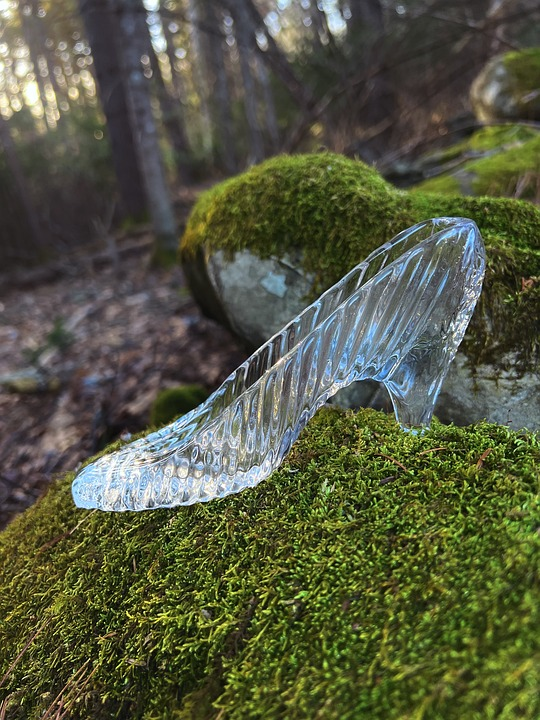
\includegraphics[width=3.20455in,height=4.27009in]{./imgSAEB_6_POR/media/image9.jpeg}
\caption{Sapatinho de cristal.}
\end{figure}

\num{1} Enumere os fatos do texto 1, de acordo com a ordem cronológica
dos acontecimentos.

\begin{boxlist}
\boxitem{1} Uma das esposas do chefe morre.
\boxitem{8} O filho do chefe manda buscar a donzela.
\boxitem{5} A menina encontra, perto do poço, um sapo.
\boxitem{7} O sapo impõe a condição de que, quando os bailarinos estiverem se
dispersando, a moça vá para casa e deixe o sapatinho de ouro no lugar.
\boxitem{4} Sem poder fazer nada, a menina vai até o poço comer as raspas de
alimento que a madrasta deixava para ela.
\boxitem{6} O sapo engole e vomita a menina, fornecendo-lhe roupas e joias para
que ela possa ir ao festival.
\boxitem{3} Certo dia, a garota queria ir a um festival, porém não tinha roupas
boas o suficiente para se vestir.
\boxitem{2} A filha do chefe é feita de empregada por sua madrasta.
\end{boxlist}

\num{2} O texto 2 apresenta apenas uma imagem e uma legenda. O que essa
imagem representa? Por que ela foi escolhida?

\reduline{A imagem do texto 2 é o sapato de cristal, que remete à
história da Cinderela. Ela foi escolhida porque o sapatinho de cristal é
o ícone que representa a Cinderela: por causa dele o príncipe descobre
com quem deve se casar no desfecho da história.\hfill}\linhas{1}

\num{3} Quais são as principais semelhanças entre o texto 1 e o conto de
fadas representado pela imagem do texto 2?

\reduline{Tanto a história do texto 1 quanto a história da Cinderela
tratam de uma princesa que, após a morte da mãe, é feita de empregada
pela madrasta. Em ambos os casos, uma criatura mágica oferece-lhe ajuda
para que ela possa ir a uma festa e nas duas histórias a personagem
abandona um sapato.\hfill}\linhas{1}

\num{4} Assinale verdadeiro (V) ou falso (F) sobre o que torna o texto 1
diferente do conto de fadas referido no texto 2.

\begin{boxlist}
\boxitem{V} O texto 1 é escrito conforme lendas e referências típicas da cultura
africana.
\boxitem{V} O texto 2 dá ênfase ao sapato de cristal, ao passo que no texto 1
esse sapato é de ouro.
\boxitem{F} No texto 1, a filha do chefe apenas deseja ir ao Festival da
Colheita.
\boxitem{V} No texto 2, a personagem é uma princesa e deseja ir a uma festa no
castelo.
\boxitem{F} O texto 1 deixa claro que a filha do chefe é maltratada pela
madrasta e suas duas meia-irmãs.
\boxitem{F} O elemento místico no texto 1 está no fato de os sapos falarem, ao
passo que no texto 2 está no fato de haver uma fada-madrinha.
\end{boxlist}


Leia os textos seguir e resolva as atividades de 5 a 7.

\textbf{TEXTO I}

\noindent Veja a imagem de um meme e leia o texto que a acompanha.

\begin{figure}[H]
%PORT_6_IMG-16 — POR.tex:1215
\centering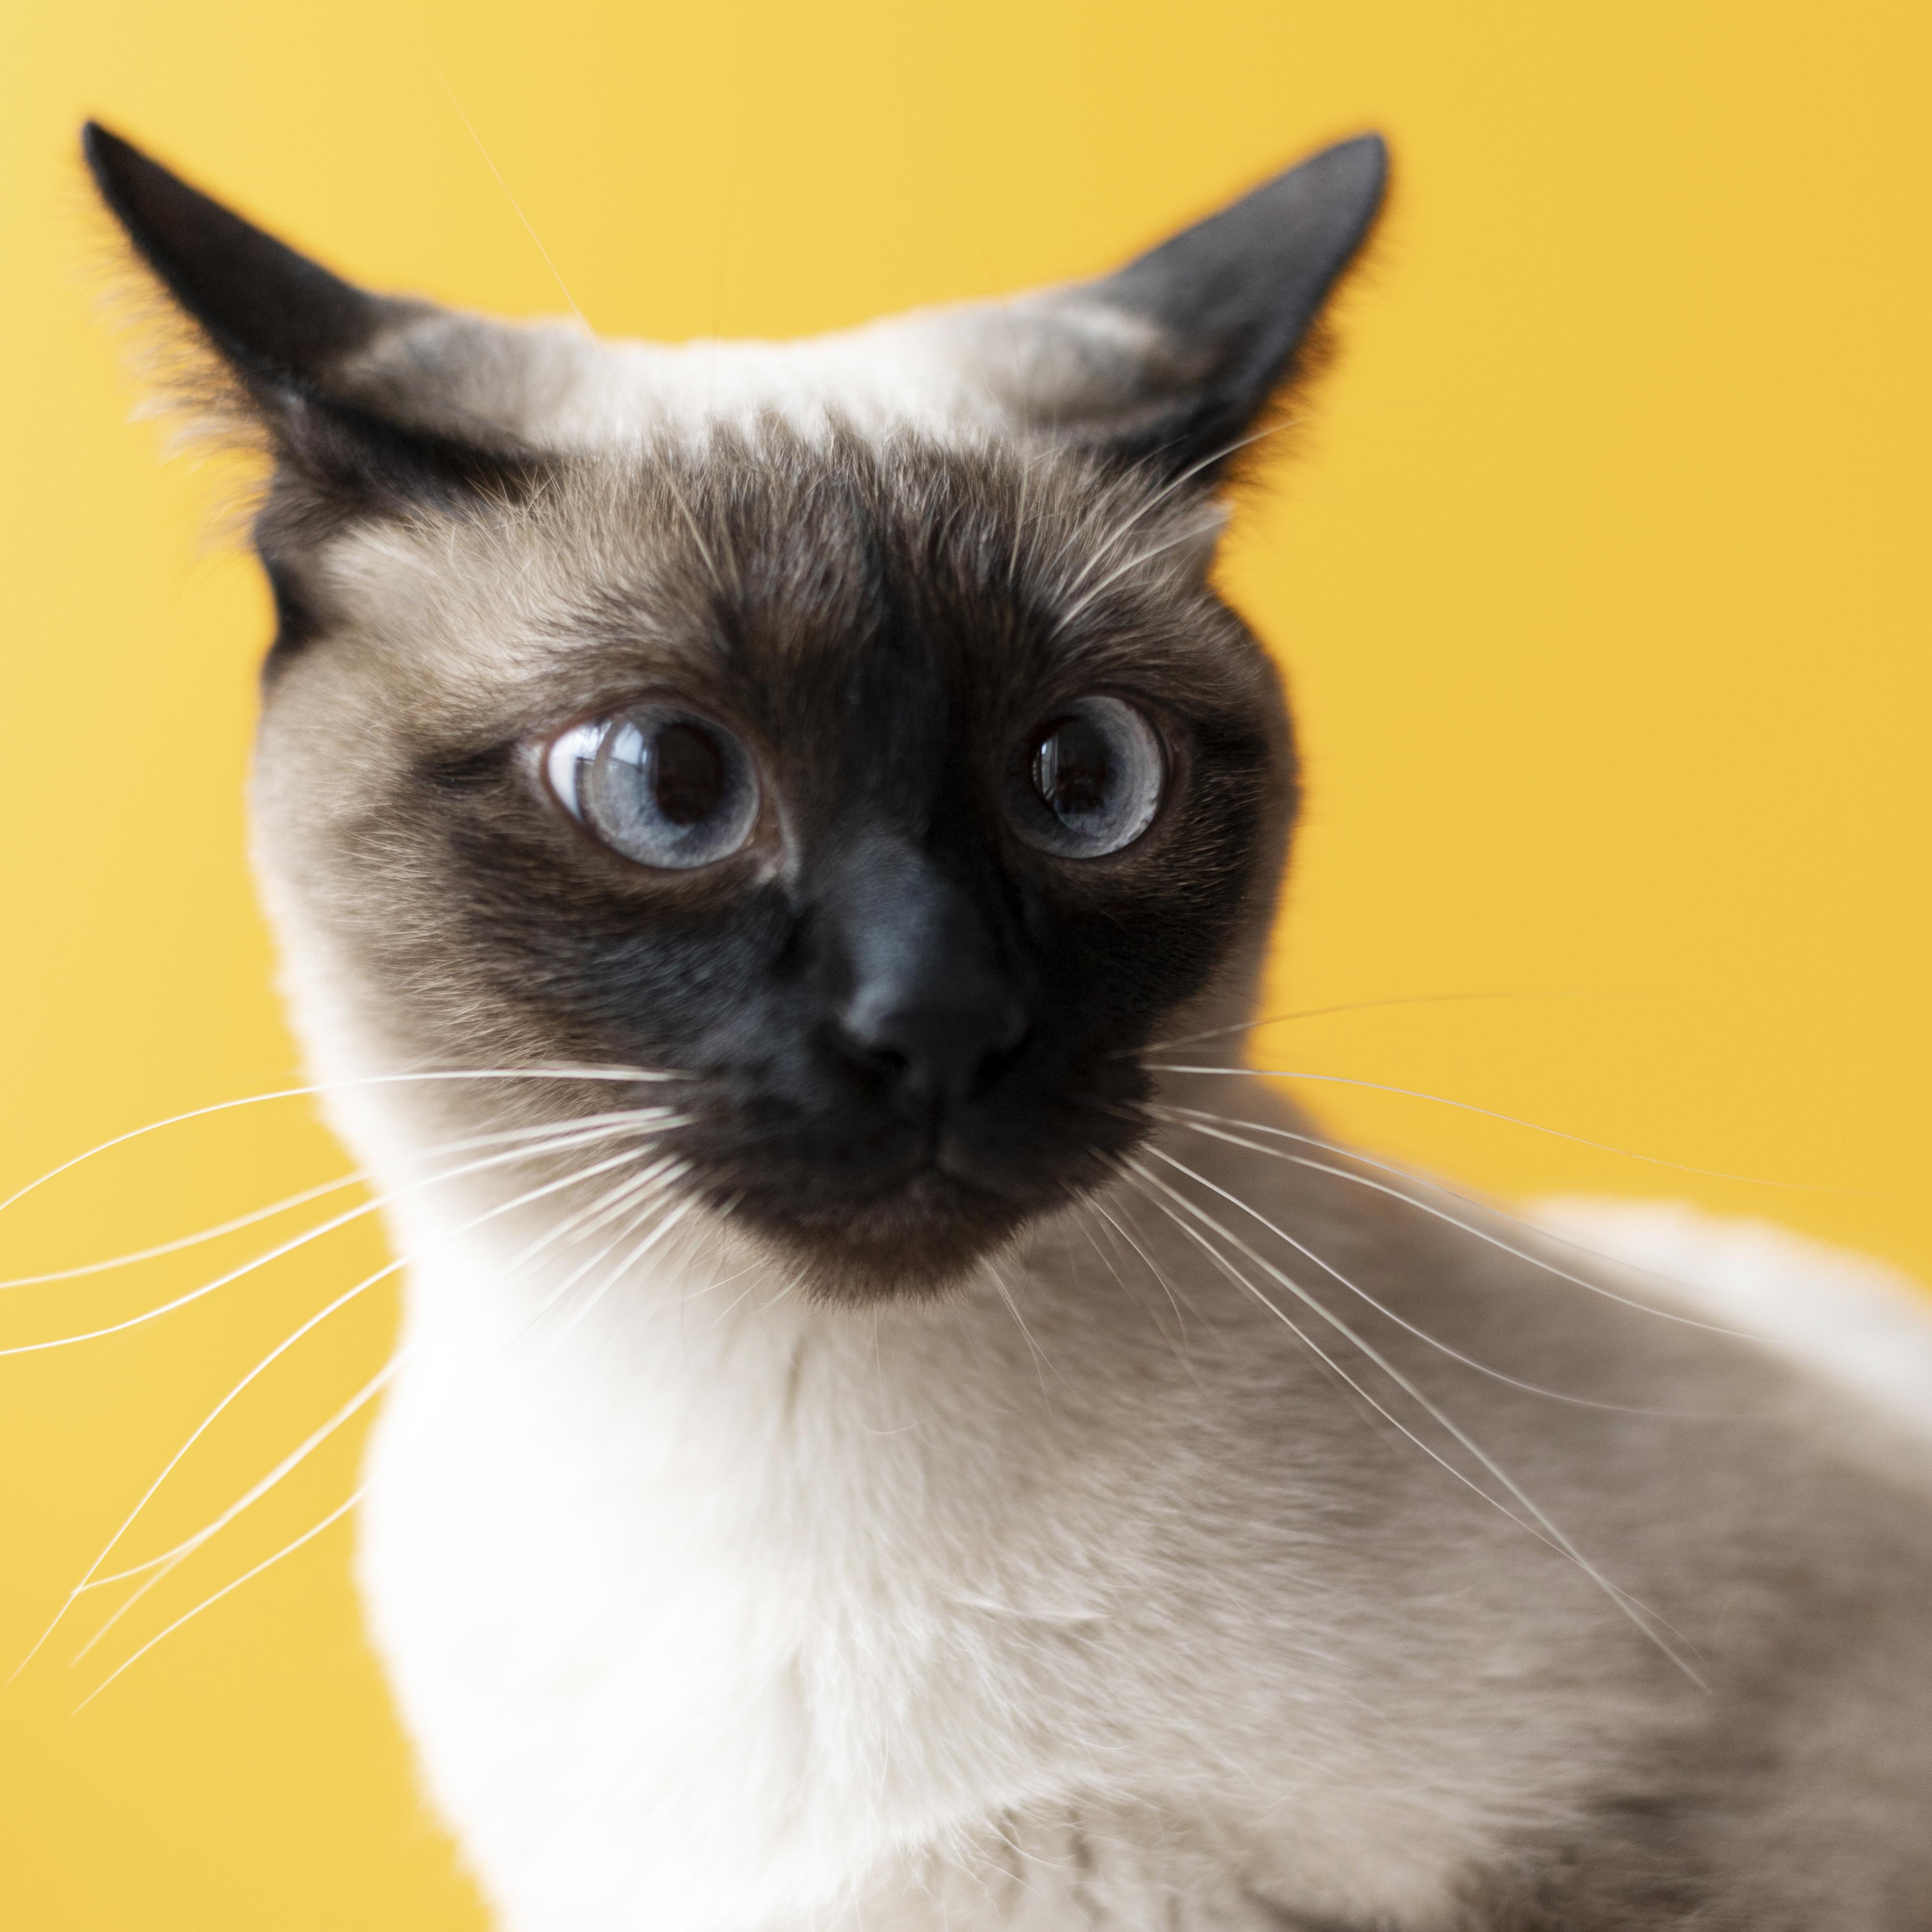
\includegraphics[width=0.7\textwidth]{./imgSAEB_6_POR/freepik/PORT_6_IMG-16.jpeg}
\end{figure}

\begin{quote}
Olhos de cigana, oblíqua e dissimulada.

(Machado de Assis, \emph{Dom Casmurro}.)
\end{quote}


\begin{quote}
\textbf{TEXTO II}

Juro! Deixe ver os olhos, Capitu.\\
Tinha-me lembrado a definição que José Dias dera deles, ``olhos de cigana
oblíqua e dissimulada.'' Eu não sabia o que era oblíqua, mas dissimulada
sabia, e queria ver se podiam chamar assim. Capitu deixou-se fitar e
examinar. Só me perguntava o que era, se nunca os vira; eu nada achei
extraordinário; a cor e a doçura eram minhas conhecidas.

(Machado de Assis, \emph{Dom Casmurro})
\end{quote}


\begin{tabular}{ll}
\textbf{Glossário} & \mbox{}\\
Oblíqua & inclinada; diagonal; maldosa.\\
Dissimulada & pessoa fingida, falsa.\\
Fitar & olhar; admirar.\\
\end{tabular}


\num{5} Qual é o efeito de sentido que a palavra ``oblíqua'' adquire no
contexto do texto I?

\reduline{A palavra adquire um sentido real, já que os olhos do gatinho
são realmente inclinados, na diagonal.\hfill}\linhas{1}

\num{6} Por que a palavra ``dissimulada'' faz sentido no texto I?

\reduline{ Porque é um senso comum algumas pessoas associarem gatos a
seres traiçoeiros.\hfill}\linhas{1}

\num{7} A que se refere o pronome ``os'', no trecho ``Só me perguntava o
que era, se nunca os vira'', extraído do texto II?

\reduline{ O pronome se refere aos olhos de Capitu.\hfill}\linhas{1}

\noindent Observe a imagem e leia o texto que a acompanha, a seguir, para
resolver as atividades de 8 a 10.

%
\includegraphics[width=5.90556in,height=4.43889in]{./imgSAEB_6_POR/media/image11.png}

\begin{figure}[H]
%PORT_6_IMG-17 — POR.tex:1258
\centering
\includegraphics[width=0.7\textwidth]{./imgSAEB_6_POR/freepik/PORT_6_IMG-17.jpeg}
\caption{De mal\ldots{} a pior.}
\end{figure}


\num{8} A imagem apresenta uma rota cruzando o planeta Terra de um ponto
a outro, com o texto ``De mal\ldots{} a pior.''. Explique o uso das
reticências e do ponto-final nesse texto.

\reduline{ As reticências dão ao leitor a ideia de que o texto, no ponto
de partida "De mal", continua até um destino, "pior.". Elas dão ao texto
um ar misterioso, para que o leitor tenha curiosidade de saber o nome do
destino. O ponto-final encerra a frase da mesma forma como um destino.\hfill}\linhas{1}

\num{9} Observe que o pontilhado que forma a rota da origem ao destino é
uma linha curvada para baixo, de modo que o planeta parece estar triste.
Esse detalhe é proposital na composição da imagem? Qual é a função desse
recurso não verbal para o leitor?

\reduline{Esse detalhe é proposital, pois a imagem de modo geral compõe
a rota com os ícones e os pontilhados como se o planeta tivesse um rosto
humano triste — ou, até mesmo, um emoji triste. Esse recurso ajuda a
contextualizar sobre a produção do texto: o que vai de mal a pior? A
resposta seria o planeta Terra.\hfill}\linhas{1}

\num{10} A imagem faz intertextualidade com

\begin{escolha}
\item uma canção popular.
\item um ditado popular. 
\item uma figura de linguagem.
\item uma cantiga popular.
\end{escolha}

% Gabarito, treino?
% \coment{
% \begin{enumerate}
% \def\labelenumi{\alph{enumi})}
% \item Incorreta. Embora a expressão ``de mal a pior'' esteja presente em
% algumas canções da MPB, ela é um ditado popular.
% \item Correta. A frase da imagem é um ditado popular: "de mal a pior",
% usada quando se quer dizer que não há nada tão ruim que não possa
% piorar.
% \item Incorreta. De mal a pior é um ditado, uma expressão popular, e não
% uma figura de linguagem. Aqui, na imagem, seu uso pode ser associado a
% uma ironia, para dar o efeito de sentido de humor, mas o texto em si é
% um dito popular.
% \item ``De mal a pior'' não aparece em nenhuma cantiga popular.
% \end{enumerate}}

\section{Treino}

\num{1} Observe os dois textos a seguir.

\textbf{Texto 1}

\begin{figure}[H]
%PORT_6_IMG-18 — POR.tex:1309
\centering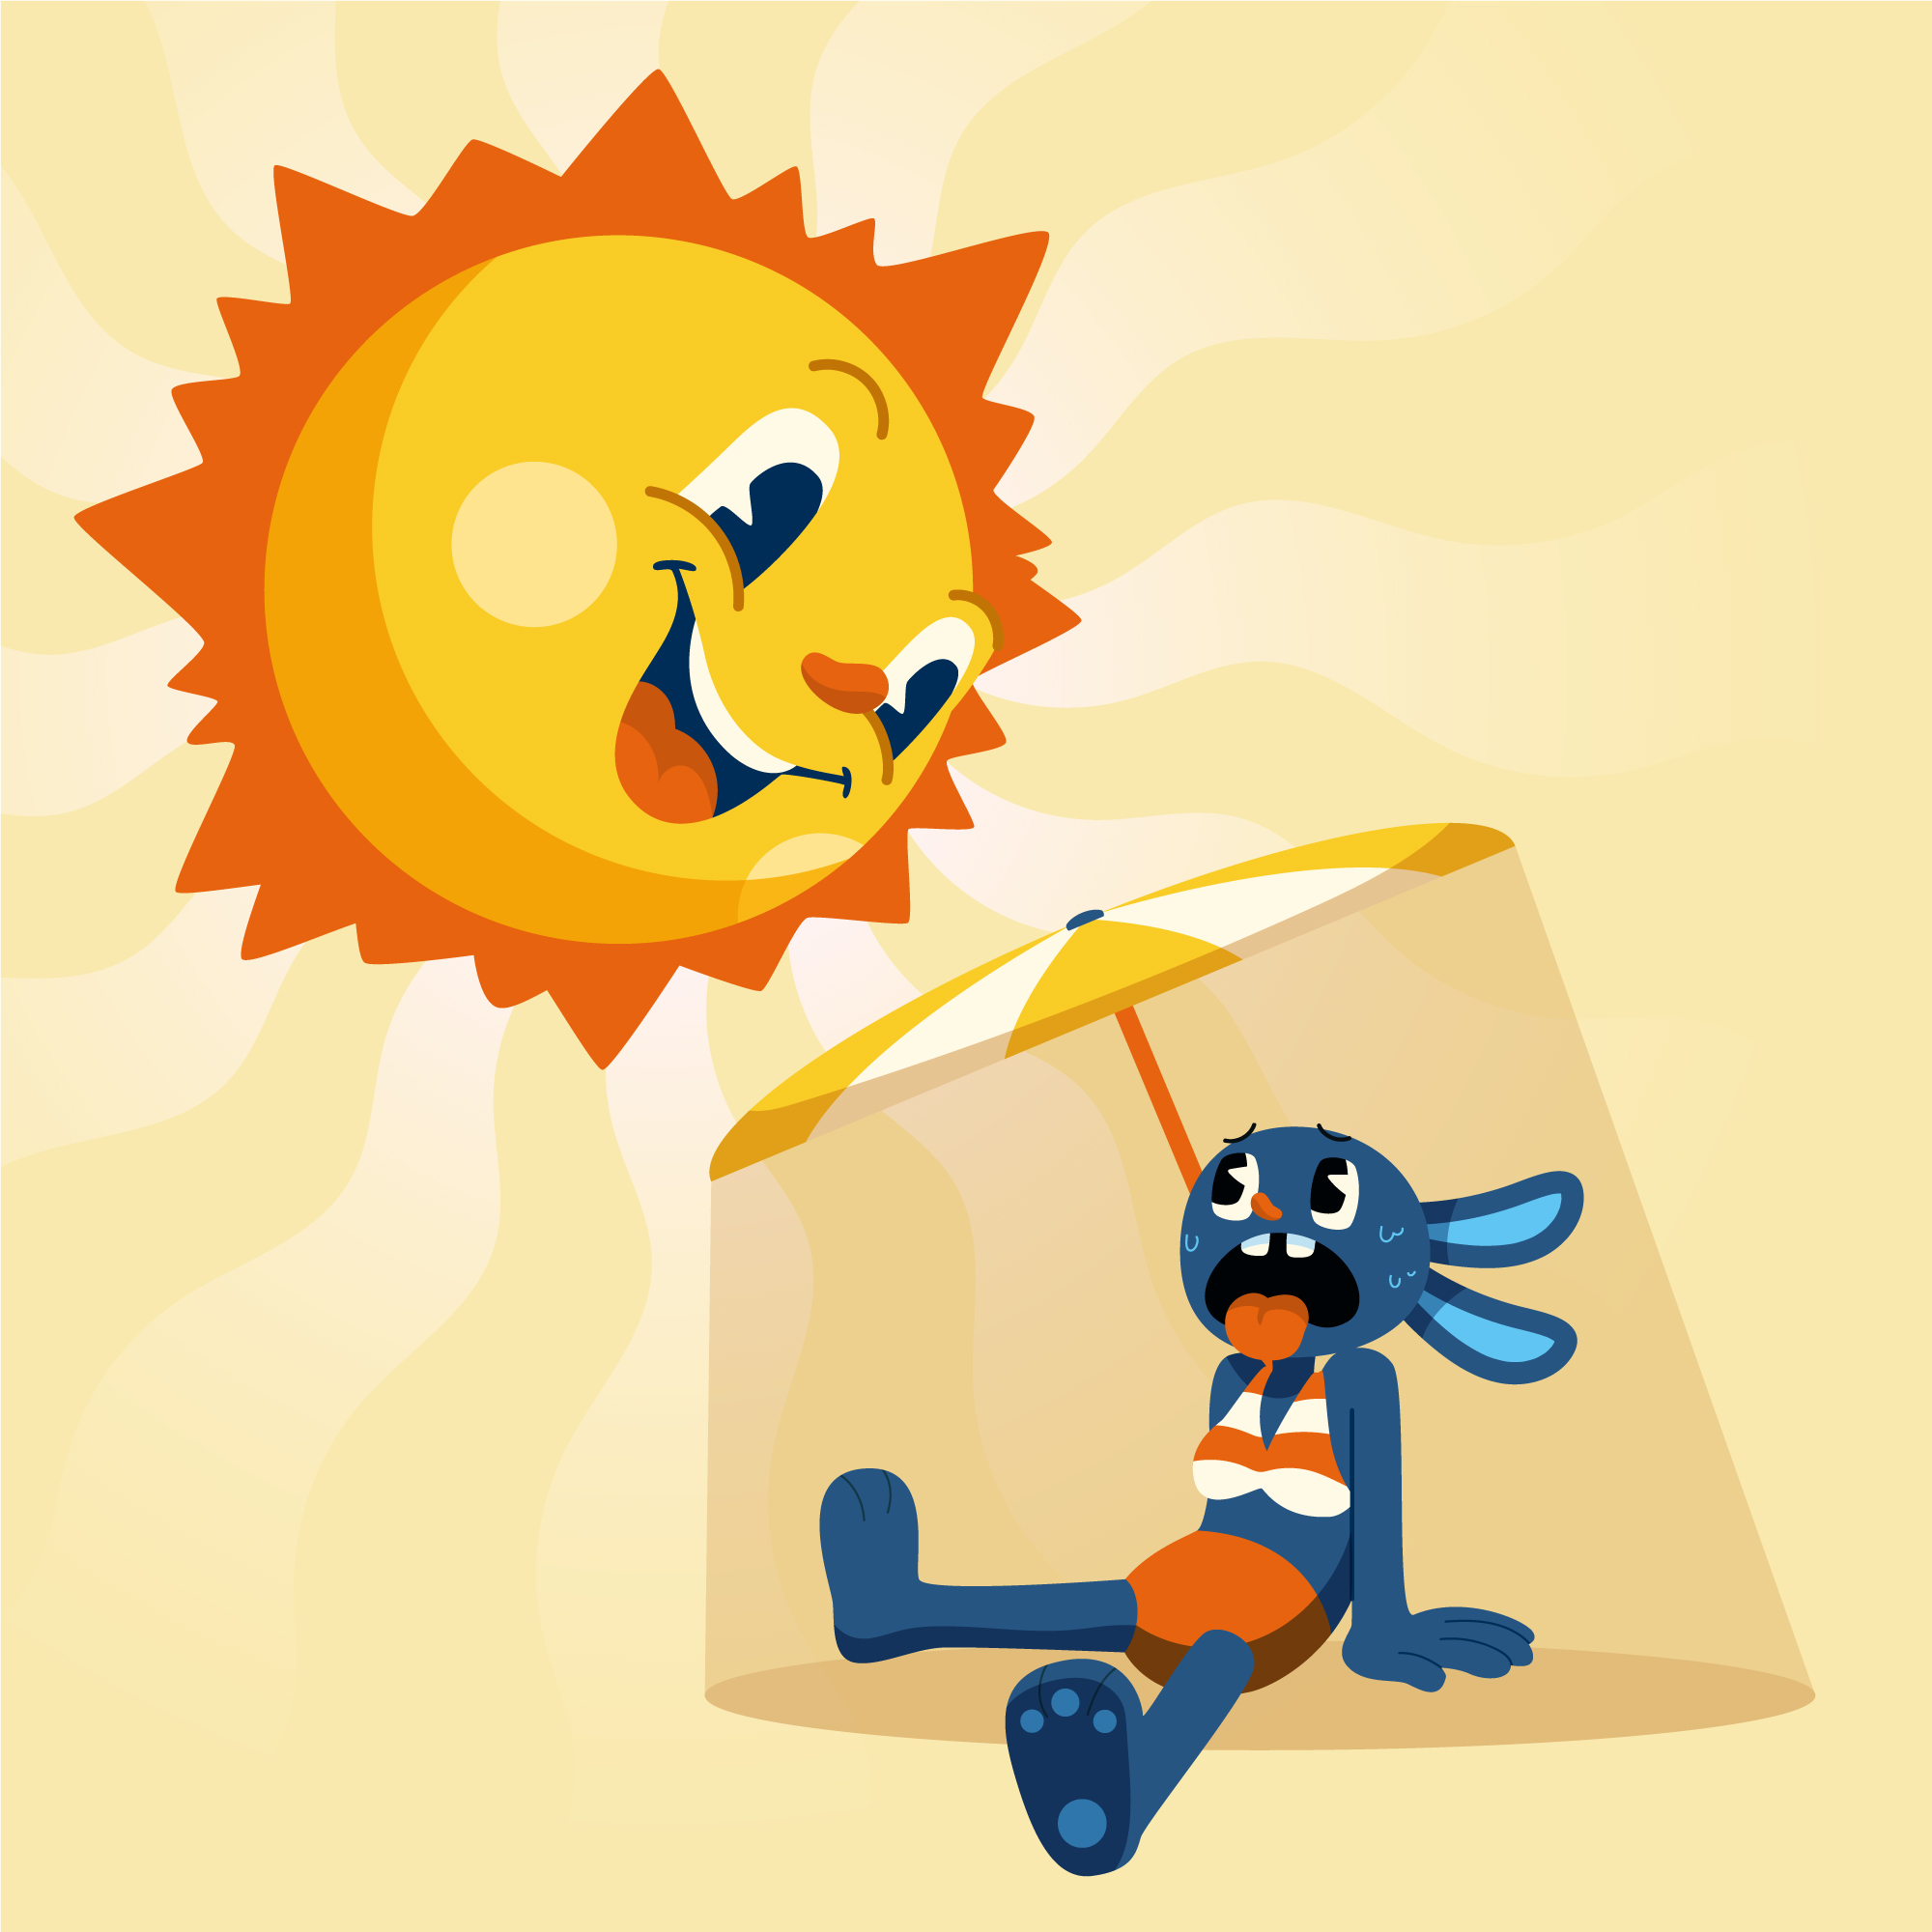
\includegraphics[width=0.7\textwidth]{./imgSAEB_6_POR/freepik/PORT_6_IMG-18.jpeg}
\end{figure}

\begin{center}
--- Tudo bem que você é essencial, mas tem hora que precisamos de uma
trégua, seu Hélio.
\end{center}

\begin{quote}
\textbf{Texto 2}

\centering\textbf{O que acontece se o Sol deixar de brilhar?}

Se o sol deixasse de brilhar, teríamos consequências catastróficas na
Terra. O sol é a estrela central do nosso sistema solar e é responsável
por fornecer a luz e o calor necessários para sustentar a vida em nosso
planeta.

Sem a luz do sol, os dias ficariam completamente escuros. Isso afetaria
diretamente a fotossíntese das plantas, que dependem da luz solar para
produzir seu próprio alimento. Com a interrupção da fotossíntese, as
plantas não conseguiriam sobreviver e, consequentemente, toda a cadeia
alimentar seria afetada.

Além disso, a temperatura na Terra diminuiria drasticamente. O sol é uma
fonte de calor vital para manter o equilíbrio térmico do nosso planeta.
Sem a sua radiação, a temperatura média da Terra cairia rapidamente,
resultando em um resfriamento global. Isso poderia levar a condições
extremamente frias, com o congelamento de rios, lagos e oceanos.

A falta de luz solar também afetaria o clima e os padrões atmosféricos.
A energia solar desempenha um papel fundamental na formação de correntes
de ar e na circulação atmosférica. Sem o calor do sol, os padrões
climáticos seriam alterados, levando a eventos climáticos extremos e
imprevisíveis.

Em resumo, se o sol deixasse de brilhar, enfrentaríamos uma crise global
sem precedentes, com a interrupção da fotossíntese, resfriamento global
e mudanças climáticas drásticas. Felizmente, essa é uma situação
extremamente improvável, já que o sol continuará a brilhar e fornecer
energia por bilhões de anos.

\fonte{Guilherme Pedroso Teixeira.}
\end{quote}

Os textos 1 e 2:

\begin{escolha}
\item Pertencem ao gênero texto de divulgação científica.
\item Apresentam intertextualidade quanto ao tema. 
\item Não têm qualquer relação.
\item São de cunho informativo.
\end{escolha}

%\paragraph{BNCC: EF67LP27} 
% Analisar, entre os textos literários e entre estes e
% outras manifestações artísticas (como cinema, teatro, música, artes
% visuais e midiáticas), referências explícitas ou implícitas a outros
% textos, quanto aos temas, personagens e recursos literários e
% semióticos.

% Gabarito, treino?
% \begin{enumerate}
% \item Incorreta. O texto 1 é um cartum e o texto 2 é um texto de divulgação
% científica.
% \item Os textos apresentam intertextualidade com relação ao tema, que é a
% influência do Sol na Terra.
% \item Incorreta. Os textos apresentam a mesma temática geral.
% \item Incorreta. Apenas o texto 2 é de cunho informativo, pois transmite a
% mensagem de maneira assertiva.
% \end{enumerate}

\pagebreak

\num{2} Observe a imagem a seguir.

\begin{figure}[H]
\centering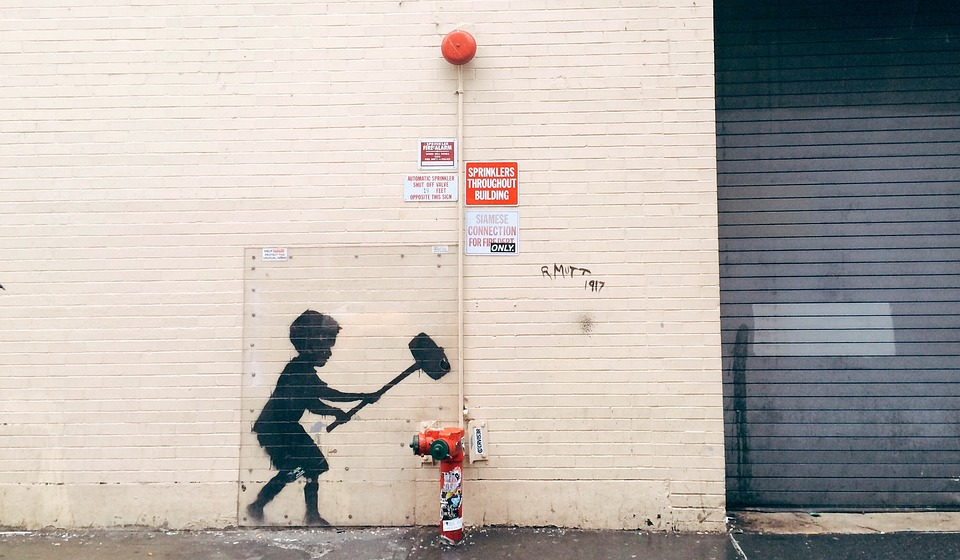
\includegraphics[width=4.69016in,height=2.73611in]{./imgSAEB_6_POR/media/image13.jpeg}
\end{figure}

A intertextualidade da obra de arte ocorre

\begin{escolha}
\item A partir da fusão de elementos cotidianos com linguagem não verbal.
\item Por meio da ilustração de como acionar o alerta sonoro presente no
muro.
\item A partir da representação de um menino brincando com um martelo que
mede a força.
\item A partir da composição de elementos verbais e não verbais, como a
pintura e os quadros de aviso.
\end{escolha}

%\paragraph{BNCC: EF67LP27} 
% — Analisar, entre os textos literários e entre estes e
% outras manifestações artísticas (como cinema, teatro, música, artes
% visuais e midiáticas), referências explícitas ou implícitas a outros
% textos, quanto aos temas, personagens e recursos literários e
% semióticos.

% Gabarito, treino?
% \begin{escolha}
% \item Incorreta. Os elementos não verbais da imagem não se dissociam de
% elementos cotidianos; eles fazem parte deles.
% \item Incorreta. A obra não pretende instruir como acionar o alerta sonoro.
% \item Correta. A imagem forma uma intertextualidade ao unir o sinal sonoro,
% na parede, com um hidrante, no chão, e a pintura do garoto brincando com
% um martelo que mede a força.
% \item Incorreta. Os elementos verbais, como os quadros na parece, não fazem
% diferença na composição da imagem.
% \end{enumerate}

\num{3} Observe a imagem a seguir.

\begin{figure}[H]
\centering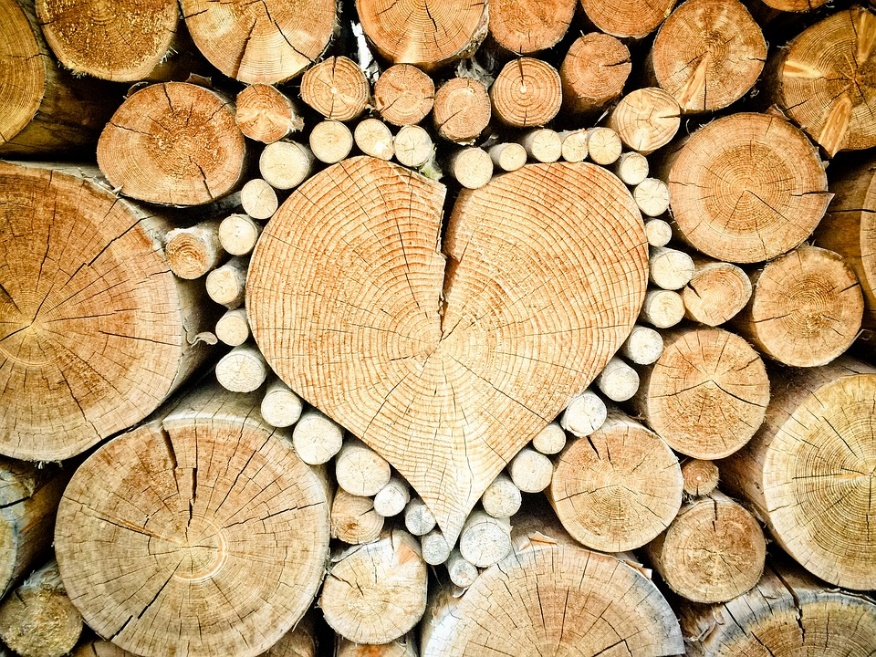
\includegraphics[width=3.97917in,height=2.98438in]{./imgSAEB_6_POR/media/image14.jpeg}
\end{figure}

A canção que formaria uma intertextualidade com a imagem é:

\begin{escolha}
\item ``Herdeiros do futuro'', de Toquinho, cujos versos questionam se a
terra continuará a fornecer frutos à humanidade.
\item ``Coração bandido'', de Maiara e Maraísa, em que se afirma que o
coração do eu é bandido por trair seu amor.
\item ``Coração de ferro'', de Zé Henrique e Gabriel, em que se fala de um
coração isento de sentir.
\item ``Natureza distraída'', de Toquinho, em que se fala de como devemos,
como as plantas, de carinho e de crescer.
\end{escolha}

%\paragraph{BNCC: EF67LP27} 
% — Analisar, entre os textos literários e entre estes e
% outras manifestações artísticas (como cinema, teatro, música, artes
% visuais e midiáticas), referências explícitas ou implícitas a outros
% textos, quanto aos temas, personagens e recursos literários e
% semióticos.

% Gabarito, treino?
% \begin{escolha}
% \item Incorreta. Embora a letra fale sobre mata, caule e raiz, não se pode
% afirmar que a imagem é de um desmatamento.
% \item Incorreta. A letra é uma canção de amor entre pessoas, e não sobre
% natureza, portanto, não apresenta intertextualidade com a imagem.
% \item Incorreta. A letra fala apenas de sentimentos humanos, e não
% apresenta intertextualidade com a imagem.
% \item Correta. A imagem apresenta um caule cortado em formato de coração,
% comparando o sentimento com a mata.
% \end{enumerate}

\chapter{Palavra do especialista}
\markboth{Módulo 4}{}

\section{Habilidades do SAEB}
\begin{itemize}
\item Analisar efeitos de sentido produzido pelo uso de
formas de apropriação textual (paráfrase, citação etc.).
\item Analisar os
efeitos de sentido decorrentes dos mecanismos de construção de textos
jornalísticos/midiáticos.
\end{itemize}

\subsection{Habilidades da BNCC}
\begin{itemize}
\item EF69LP16
\item EF69LP43
\end{itemize}

\conteudo{
As citações de terceiros em textos são uma prática comum na escrita
acadêmica e literária, permitindo que o autor apresente ideias e
informações de outras fontes e dê crédito apropriado ao autor original.
Sua utilização permite dar mais credibilidade e embasamento ao seu
texto, dando mais força aos argumentos, pois permite que você utilize
ideias, conceitos ou informações de outras fontes renomadas.

Existem diferentes maneiras de fazer uma citação, mas é importante
seguir as normas estabelecidas pelas instituições de ensino ou
publicações científicas. Algumas das formas mais comuns de citação são:

\paragraph{Citação direta} quando você transcreve exatamente as palavras de um
autor, utilizando aspas ou recuo de parágrafo. É importante indicar o
nome do autor, o ano de publicação e a página da citação.

\paragraph{Citação indireta} quando você utiliza a ideia ou informação de um
autor, mas escreve com suas

\paragraph{Citação de citação} quando você utiliza uma citação que foi citada
por outro autor. Neste caso, é importante indicar o nome do autor
original e do autor que está citando, além do ano de publicação.

\paragraph{Paráfrase} quando você produz um texto com base em outro que já
existe e é conhecido por outras pessoas, mantendo a ideia do texto
original.

Independentemente do tipo de citação escolhido, é importante sempre
indicar a fonte utilizada na lista de referências ou bibliografia do seu
trabalho.}

\section{Atividades}

\noindent Utilize o texto a seguir para resolver as atividades de 1 a 7.


\begin{quote}
\centering\textbf{Como os gatos veem o mundo}


Frente a investimentos financeiros e emocionais significativos, muitas
pessoas atribuem características humanas aos seus gatos. No entanto,
estão equivocadas. Ao contrário dos cães, que desejam ser como os
humanos, os gatos não aspiram a ser outra coisa senão gatos. Na
perspectiva felina, somos nós, seus donos, os gigantes amigáveis da
mesma espécie, encarregados de sustentá-los e protegê-los.

Protegê-los de quê? Para o gato, cada cômodo é uma selva, que ele
percebe apenas em tons de amarelo e azul. Há uma ameaça escondida atrás
de cada cortina e sob cada almofada. Eles nascem, morrem e dão origem a
predadores. Segundo John Bradshaw, autor do livro ``Sentido de gato, o
enigma felino revelado'' (best-seller de 2013 sem edição brasileira),
``eles descendem de felinos territoriais e solitários que aceitaram a
coexistência com outros gatos e ainda estão se adaptando à vida como
animais de estimação''.

Em outras palavras, aquilo que os ratos sabiam e os pufes suspeitavam, a
ciência agora confirma: o gato doméstico ainda preserva sua natureza
selvagem.

\fonte{Alexandre Rodrigues. Superinteressante. \emph{Como os gatos veem o mundo}. Disponível em: https://super.abril.com.br/ciencia/como-os-gatos-veem-o-mundo. Acesso em: 9 mar. 2023.}
\end{quote}

\num{1} O título de tem a função de apresentar ao leitor o tema que será
trabalhado no texto. No caso desse artigo, se considerarmos que o verbo
``ver'' está empregado em seu sentido denotativo, ou seja, literal, que
tipo de informação o leitor pode esperar, antes de ler o texto?

\linhas{3}

\reduline{ O leitor espera compreender mais sobre como funciona a visão
dos gatos, ou seja, como eles enxergam.\hfill}\linhas{1}

\pagebreak

\num{2} Após a leitura do texto, qual é o efeito de sentido que o verbo
``veem'' adquire no título? Justifique sua resposta.

\linhas{5}

\reduline{O verbo tem o sentido de compreender, pois o texto não fala
apenas do modo como os gatos enxergar, mas sim como eles entendem o
mundo ao seu redor.\hfill}\linhas{1}

\num{3} Qual é a tese apresentada no texto? Copie o trecho que apresenta
essa informação.

\reduline{A tese é de que os gatos domésticos ainda são animais
selvagens. O trecho que confirma essa informação é: ``Ao contrário dos cães, que desejam ser como os humanos, os gatos não aspiram a ser outra coisa senão gatos.''\hfill}\linhas{1}

\num{4} Que tipos de argumentos o autor utiliza para defender essa tese?

\reduline{O autor utiliza comparações e referências da convivência cotidiana com os gatos, como em "Há uma ameaça escondida atrás de cada cortina e sob cada almofada.", além do trecho que apresenta a citação de um autor especialista, John Bradshaw.\hfill}\linhas{1}

\num{5} Por que o auxtor do artigo reproduz a fala de um especialista no
desenvolvimento do texto?

\reduline{Porque a fala do especialista dá credibilidade ao texto.\hfill}\linhas{1}

\num{6} As aspas utilizadas em ``eles descendem de felinos territoriais
e solitários que aceitaram a coexistência com outros gatos e ainda estão
se adaptando à vida como animais de estimação''

\begin{escolha}
\item Reproduzem a fala do especialista na forma de discurso indireto. 
\item Reproduzem a fala do especialista na forma de discurso direto.
\item Dão destaque à tese de que os gatos são felinos selvagens.
\item Dão destaque ao fato de um especialista ter sido entrevistado.
\end{escolha}

% Gabarito, treino?
% \coment{
% \begin{enumerate}
% \def\labelenumi{\alph{enumi})}
% \item A resposta correta é "a". As aspas reproduzem a fala do especialista na forma de discurso indireto.
% \item  Incorreta. O discurso direto é representado por meio de travessão e
% quebra de parágrafo.
% \item  Incorreta. A função das aspas, aqui, é demarcar o que foi
% reproduzido da fala do especialista.
% \item  Incorreta. O fato de um especialista ter sido entrevistado apenas
% não exige por si só que o trecho em que isso é mencionado seja usado
% entre aspas.
% \end{enumerate}}

\num{7} Além as aspas, qual é o recurso utilizado no texto para que o
leitor reconheça a frase do especialista como uma citação?

\reduline{O conector *segundo*, que precede trecho entre aspas.\hfill}\linhas{1}

\noindent Leia o texto a seguir para resolver as atividades de 8 a 10.

\begin{quote}
{[}\ldots{]} Todo mundo conhece a música Ciranda-Cirandinha. A Adriana,
uma amiga, me confessou que durante anos e anos, entendia um verso
completamente diferente. Quando a letra fala~o amor que tu me tinhas era
pouco e se acabou, ela achava que era~o amor de Tumitinha era pouco e se
acabou. Tumitinha era um menino, coitado. {[}\ldots{]}

\fonte{Mário Prata. \emph{O amor de Tumitinha}. Disponível em: https://marioprata.net/cronicas/o-amor-de-tumitinha. Acesso em: 3 mar. 2023.}
\end{quote}

\num{8} Qual é o motivo da confusão entre o verso e a maneira como ele
foi compreendido?

\reduline{A sonoridade parecida entre as palavras "tu me tinhas" e o nome imaginado por ela ``Tumitinha''.\hfill}\linhas{1}

\num{9} Qual é o recurso utilizado pelo autor para que as pessoas saibam
que a história que ele reconta é, na verdade, inventada pela sua amiga?

\reduline{O autor menciona, no começo do texto, que sua amiga Adriana
confessou que entendia a letra de Ciranda-cirandinha de outro jeito.\hfill}\linhas{1}

\num{10} Qual é o efeito de sentido que o verbo ``confessar'' provoca
nesse caso?

\reduline{O verbo confessar deixa evidente que o fato era, até então, um
segredo da amiga do autor do texto, algo que ela tinha vergonha de
falar. Por isso ele informa que ela "confessou" que cantava errado.\hfill}\linhas{1}

\section{Treino}

\num{1} Observe a imagem e leia o texto que, juntos, compõem um informe
visual.

\begin{figure}[H]
%PORT_6_IMG-19 — POR.tex:1659
\centering
\includegraphics[width=0.7\textwidth]{./imgSAEB_6_POR/freepik/PORT_6_IMG-19.jpeg}
\end{figure}

%colocar a imagem de ``cabeça para baixo'', de forma que o cérebro
%pareça um coração. 

\begin{quote}
Para manter sua saúde mental em dia, você precisa: 

\begin{escolha}
\item Praticar exercícios; 
\item Manter uma alimentação saudável; 
\item Aproveitar passeios e caminhadas ao ar livre;
\item Dormir 8 horas por dia; 
\item Conversar sobre o que sente com pessoas de confiança; 
\item Procurar ajuda profissional se for preciso; 
\item Manter uma alimentação saudável e diversificada.
\end{escolha}
\end{quote}

Qual é a tese apresentada no informe?

\begin{escolha}
\item Saúde mental e saúde física caminham juntas. 
\item Para ter saúde mental, basta seguir as dicas relacionadas à atividade física.
\item Não é possível ter saúde mental se todas as dicas não forem seguidas.
\item A saúde mental só depende da pessoa.
\end{escolha}

%\paragraph{BNCC: EF69LP43} 
% Identificar e utilizar os modos de introdução de outras vozes no texto — citação literal e sua formatação e paráfrase --, as pistas linguísticas responsáveis por introduzir no texto a posição do autor e dos outros autores citados (``Segundo X; De acordo com Y; De minha/nossa parte, penso/amos que''\ldots) e os elementos de normatização (tais como as regras de inclusão e formatação de citações e paráfrases, de organização de referências bibliográficas) em textos científicos, desenvolvendo reflexão sobre o modo como a intertextualidade e a retextualização ocorrem nesses textos.

% Gabarito, treino?
% \begin{enumerate}
% \def\labelenumi{\alph{enumi})}
% \item Correta. O informe apresenta dicas de saúde mental que englobam
% comportamentos que auxiliam na manutenção do físico e do psicológico.
% \item Incorreta. As informações do infográfico são dicas, sugestões, e não
% necessariamente bastam para se ter saúde mental.
% \item Incorreta. Não se pode afirmar que não é possível ter saúde mental se
% essas dicas não forem seguidas.
% \item Incorreta. A saúde mental depende de uma série de circunstâncias. O
% infográfico apresenta apenas algumas dicas.
% \end{enumerate}

\num{2} Leia a reportagem a seguir.


\begin{quote}
\centering\textbf{Como cuidar da saúde mental das crianças?}


Os primeiros anos de vida desempenham um papel fundamental na formação
das habilidades cognitivas que o cérebro desenvolverá ao longo dos anos
subsequentes. Portanto, investir na promoção da saúde mental infantil é
uma maneira de cuidar do bem-estar das futuras gerações, abrangendo
desde jovens até idosos, e também de preservar o bem-estar de nossas
comunidades.

Além disso, é durante a infância que os primeiros sinais de transtornos
mentais costumam se manifestar, podendo agravar-se significativamente na
vida adulta. De acordo com a Organização Mundial da Saúde (OMS), metade
dos distúrbios mentais têm início por volta dos 14 anos de idade.
Portanto, discutir o assunto e estar bem informado sobre os sintomas
contribui para a detecção precoce dos problemas de saúde mental.

\fonte{Elen Montanari. Blog Leiturinha. \emph{Como cuidar da saúde mental das crianças?} Disponível em: https://leiturinha.com.br/blog/como-cuidar-da-saude-mental-das-criancas. Acesso em: 14 mar. 2023.}
\end{quote}

\noindent O recurso argumentativo utilizado que apoia a tese apresentada no texto é:

\begin{escolha}
\item Uma paráfrase.
\item Uma citação direta.
\item Uma citação indireta. 
\item Uma citação de citação.
\end{escolha}

%\paragraph{BNCC: EF69LP43} 
% Identificar e utilizar os modos de introdução de outras vozes no texto — citação literal e sua formatação e paráfrase --, as pistas linguísticas responsáveis por introduzir no texto a posição do autor e dos outros autores citados (``Segundo X; De acordo com Y; De minha/nossa parte, penso/amos que''\ldots) e os elementos de normatização (tais como as regras de inclusão e formatação de citações e paráfrases, de organização de referências bibliográficas) em textos científicos, desenvolvendo reflexão sobre o modo como a intertextualidade e a retextualização ocorrem nesses textos.

% Gabarito, treino?
% \begin{enumerate}
% \def\labelenumi{\alph{enumi})}
% \item Incorreta. A citação usada como argumento é indireta.
% \item Incorreta. Seria uma citação direta se o trecho estivesse
% identificado entre aspas, por exemplo.
% \item Correta. O texto apresenta a tese de que os primeiros anos de vida
% funcionam como base para as aquisições que o cérebro fará nos anos
% seguintes, portanto, promover a saúde mental infantil é uma forma de
% cuidar de nossos futuros jovens, adultos e idosos. Para argumentar, é
% utilizado como recurso uma citação indireta de um dado da OMS.
% \item Incorreta. A paráfrase ocorre com mais frequência em textos que
% demonstram que o enunciador reconta uma história, e não em artigos
% científicos.
% \end{enumerate}

\num{3} Leia o texto a seguir.

\begin{quote}
Ruth Rocha recebeu a equipe da TV Brasil em sua residência, em São
Paulo, para um papo sobre sua trajetória no universo literário e a
importância da leitura para as novas gerações.

Na entrevista, a escritora diz que é preciso conversar com as crianças
pois elas entendem mais do que se imagina. A autora conta que entende e
gosta de falar para as crianças de ontem e de hoje.

Ruth Rocha também destaca a importância do professor na formação do
público leitor. "O professor deve ler o livro antes e, se gostar, ler
para os alunos. Todos têm que gostar para dar certo", sugere a veterana
que adora ler e continua lendo de tudo.

Reverenciada pela crítica e pelo público, a autora foi reconhecida com
diversos prêmios como o Jabuti.

\fonte{Disponível em: https://tvbrasil.ebc.com.br/entrevista-com-ruth-rocha-e-destaques-no-dia-das-criancas. Acesso em: mar. 2023. Adaptado.}
\end{quote}

O trecho que apresenta uma citação indireta é

\begin{escolha}
\item Ruth Rocha recebeu a equipe da TV Brasil em sua residência, em São
Paulo, para um papo sobre sua trajetória no universo literário e a
importância da leitura para as novas gerações.
\item "O professor deve ler o livro antes e, se gostar, ler para os alunos.
Todos têm que gostar para dar certo".
\item Ruth Rocha também destaca a importância do professor na formação do
público leitor.
\item Na entrevista, a escritora diz que é preciso conversar com as
crianças pois elas entendem mais do que se imagina. 
\end{escolha}

%\paragraph{BNCC: EF69LP43} 
% Identificar e utilizar os modos de introdução de outras vozes no texto — citação literal e sua formatação e paráfrase --, as pistas linguísticas responsáveis por introduzir no texto a posição do autor e dos outros autores citados (``Segundo X; De acordo com Y; De minha/nossa parte, penso/amos que''\ldots) e os elementos de normatização (tais como as regras de inclusão e formatação de citações e paráfrases, de organização de referências bibliográficas) em textos científicos, desenvolvendo reflexão sobre o modo como a intertextualidade e a retextualização ocorrem nesses textos.

% Gabarito, treino?
% \begin{enumerate}
% \def\labelenumi{\alph{enumi})}
% \item Incorreta. O primeiro parágrafo é apenas uma introdução da matéria.
% \item Incorreta. Esta é uma citação direta, destacada entre aspas.
% \item Incorreta. Esta é uma introdução à citação direta subsequente.
% \item Correta. É possível identificar que esta é uma citação indireta a
% partir de expressões modalizadoras que representam o posicionamento da
% entrevistada; neste caso, o verbo ``dizer'' faz essa função.
% \end{enumerate}


\chapter{Fato e opinião}
\markboth{Módulo 5}{}

\section{Habilidades do SAEB}
\begin{itemize}
\item Inferir informações implícitas em distintos
textos.
\item Distinguir fatos de opiniões em textos.
\end{itemize}

\subsection{Habilidade da BNCC} 
\begin{itemize}
\item EF67LP04
\end{itemize}

\conteudo{
Opinião é uma avaliação subjetiva ou julgamento que uma pessoa faz sobre
algo, com base em sua experiência, conhecimento, crenças, valores e
emoções. É uma expressão pessoal e subjetiva de um ponto de vista, que
pode ser influenciada por diversos fatores, tais como cultura, contexto
social, educação, entre outros. Podem ser expressas de diversas formas,
como através de discursos, escritos, desenhos, fotos, vídeos, entre
outros meios. As opiniões podem ser expressas de maneira positiva,
negativa ou neutra, dependendo da perspectiva e do contexto em que são
apresentadas.

É importante lembrar que as opiniões são subjetivas e podem variar de
pessoa para pessoa, e que nem sempre são baseadas em fatos ou
evidências. Por isso, é essencial buscar elementos que comprovem a
veracidade de uma informação, avaliar as opiniões com cuidado e
considerar diferentes perspectivas antes de formar uma opinião própria
sobre um determinado assunto.}

\pagebreak

\section{Atividades}

\noindent Observe a imagem e leia o texto que a acompanha para responder às
questões de 1 a 5.

\begin{figure}[H]
\centering\noindent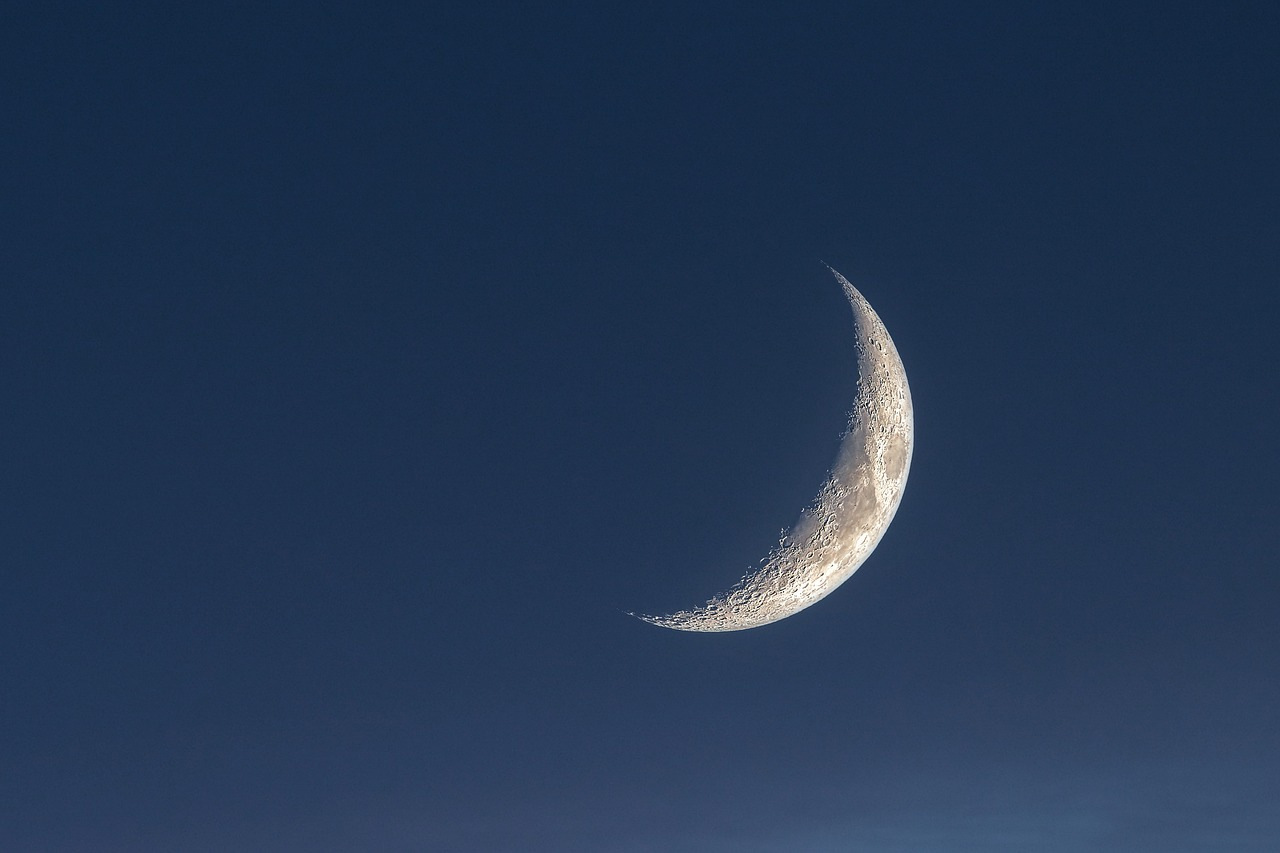
\includegraphics[width=.3\textwidth]{./imgSAEB_6_POR/freepik/PORT_6_IMG-36.jpeg}
\end{figure}

{Não há bem que para sempre dure, e não há mal que dure para sempre. (Clarice Lispector)}\medskip


\num{1} A quem é atribuída a frase relacionada à imagem?

\reduline{A Clarice Lispector.\hfill}\linhas{1}

\num{2} Qual é a função dos elementos não verbais no caso desse texto?

\reduline{A imagem da lua tem a única função de chamar a atenção para a
postagem. Ela não agrega nada para a frase.\hfill}\linhas{1}

\num{3} De que maneira uma pessoa pode descobrir se essa frase é mesmo
de Clarice Lispector? Há, na imagem, algo que forneça essa informação?

\reduline{Para ter certeza, a pessoa pode pesquisar quem é Clarice
Lispector e que tipo de frase é essa. A imagem em si não dá qualquer
pista de que a frase é realmente da autora.\hfill}\linhas{1}

\num{4} Que tipo de frase é essa? Em que contexto(s) ela circula?

\reduline{A frase é um ditado popular, de autoria desconhecida. Ela
circula de pessoa para pessoa, em muitos meios sociais específicos.\hfill}\linhas{1}

\num{5} Caso essa frase fosse mesmo dessa autora, de que maneira ela
deveria ser apresentada, para que o leitor não tenha dúvida quanto à
autoria?

\reduline{A frase deveria estar entre aspas e o nome da autora deveria
estar acompanhado da referência bibliográfica.\hfill}\linhas{1}

\noindent Leia o texto a seguir para resolver as atividades de 6 a 10.

\begin{quote}
\centering\textbf{Um mito chamado Frida Kahlo}


\noindent Após a experiência quase fatal que a deixou imobilizada por um longo
período, de acordo com relatos descritos por muitos historiadores, Frida
Kahlo teve que se reinventar. Foi então que ``pintar as coisas que via
com seus próprios olhos'' começou a fazer sentido. O espelho que estava
no teto de sua cama pode ser uma explicação contundente para os
aproximadamente 40 autorretratos que ela pintou ao longo de sua vida.

Esse ponto é o início do fascínio para muitas pessoas, pois ela pintou o
que viu sem nenhuma formação acadêmica. No entanto, é importante
destacar que, embora ela tenha retomado uma vida praticamente normal,
houve uma mudança radical após o acidente. Ela precisou utilizar
espartilhos de gesso e couro, muletas e pernas postiças. Esses elementos
não são visualmente agradáveis e não oferecem conforto no dia a dia. No
entanto, a construção de sua imagem por meio do vestuário mostrou-se uma
obra de arte por si só, algo que nenhum outro artista havia realizado
até então. Essa expressão partiu de uma necessidade interna de reafirmar
sua feminilidade.

\fonte{Tatiane Alves. Roda Cult. \emph{Um mito chamado Frida Kahlo}. Disponível em:
https://rotacult.com.br/2020/07/opiniao-um-mito-chamado-frida-kahlo/?amp.
Acesso em: 10 mar. 2023.}
\end{quote}

\num{6} Escreva, ao lado das frases, se elas se referem a um fato ou a
uma opinião sobre Frida Kahlo:

\begin{escolha}
\item Frida Kahlo teve que se reinventar. \reduline{fato.\hfill}
\item Esse ponto é o início do fascínio para muitas
pessoas \reduline{opinião.\hfill}
\item No entanto, é importante destacar que, embora ela tenha retomado
uma vida praticamente normal, houve uma mudança radical após o
acidente. \reduline{fato.\hfill}
\item Ela precisou utilizar espartilhos de gesso e couro, muletas e
pernas postiças. \reduline{fato.\hfill}
\end{escolha}

\num{7} No primeiro parágrafo, o trecho ``pintar as coisas que via com
seus próprios olhos'' está entre aspas porque:

\begin{escolha}
\item É uma frase dita por especialista em Frida Kahlo.
\item É uma paráfrase em que a autora recria o relato que muitos
historiadores descrevem. 
\item A autora pretender dar um destaque a um trecho que ela considera
importante para o entendimento do leitor.
\item A frase está em sentido figurado, ou seja, não é um fato sobre a vida
de Frida, e sim uma opinião.
\end{escolha}

% Gabarito, treino?
% \coment{
% \begin{enumerate}
% \def\labelenumi{\alph{enumi})}
% \item Incorreta. O texto não apresenta entrevista ou mesmo citação
% indireta de qualquer especialista em Frida Kahlo.
% \item Corrreta. A frase é uma paráfrase.
% \item Incorreta. O destaque dado à frase, na verdade, é uma paráfrase em
% que a autora reproduz falas comuns atribuídas a historiadores. Ela
% utiliza suas próprias palavras, porém destacando que a frase é de outra
% pessoa.
% \item Incorreto. A frase é um fato sobre Frida. Embora esteja escrito em
% sentido figurado, é fato que a partir do acidente Frida passou a pintar
% aquilo que sentia.
% \end{enumerate}}

\pagebreak

\num{8} Leia a definição da palavra \emph{mito}, segundo o dicionário
Michaelis:

\begin{quote}
Uma pessoa ou um fato cuja existência, presente na imaginação das
pessoas, não pode ser comprovada; ficção.
\end{quote}

\noindent Qual é o intuito da autora do artigo de opinião ao chamar Frida Kahlo,
uma pessoa real, de mito?

\reduline{O intuito é comparar a história de vida da autora com uma
história de ficção, quase inacreditável.\hfill}\linhas{1}

\num{9} Releia o trecho a seguir. 

\begin{quote}
No entanto, a construção de sua imagem por
meio do vestuário mostrou-se uma obra de arte por si só, algo que nenhum
outro artista havia realizado até então. Essa expressão partiu de uma
necessidade interna de reafirmar sua feminilidade.
\end{quote}

\noindent Explique, especificamente nesse trecho, o que é fato e o que é opinião.

\reduline{É fato que Frida precisou reconstruir sua imagem por meio da
vestimenta, partindo de uma necessidade interna de reafirmar sua
feminilidade. É uma opinião da autora que esse processo foi uma obra de
arte à parte.\hfill}\linhas{1}

\num{10} Explique o uso da expressão ``uma obra de arte por si só'', no
último parágrafo.

\reduline{A autora faz um trocadilho com a fato de Frida ser uma
artista. A expressão ``uma obra de arte por si só'' significa que determinado fato
foi incrível, maravilhoso.\hfill}\linhas{1}

\section{Treino}

\num{1} Leia o trecho de uma resenha crítica sobre o gibi ``Turma da
Mônica Jovem''.

\begin{quote}
``\emph{Turma da Mônica Jovem: Mudando o Jogo} tem um enredo simples,
bem curtinho e eu queria mais! É satisfatório ver que a personalidade
dos personagens se mantém, mas com certo amadurecimento constante.''

\fonte{Michele Lima. \emph{Na nossa estante}. ``Turma da Mônica Jovem: Mudando o Jogo'' {[}Resenha Literária{]}. Disponível em: 
https://nanossaestante.com.br/2022/04/turma-da-monica-jovem-mudando-o-jogo-resenha-literaria. Acesso em: mar. 2023.}
\end{quote}

A alternativa que NÃO remete a uma opinião da autora é:

\begin{escolha}
\item Tem um enredo simples.
\item E eu queria mais.
\item É satisfatório ver.
\item Mas com certo amadurecimento. 
\end{escolha}

%\paragraph{BNCC: EF67LP04} 
% Distinguir, em segmentos descontínuos de textos, fato
% da opinião enunciada em relação a esse mesmo fato.

% Gabarito, treino?
% \begin{enumerate}
% \item Incorreta. A resenhista considera o enredo simples, mas pode não ser
% simples para outras pessoas.
% \item Incorreta. Querer ler mais é uma opinião da autora.
% \item Incorreta. É satisfatório para a autora ver que a personalidade das
% personagens se mantém.
% \item Correta. O fato de as personagens apresentarem certo amadurecimento
% não é uma opinião da resenhista, e sim uma constatação.
% \end{enumerate}

\num{2} Leia o texto a seguir.

\begin{quote}
\textbf{O Brasil precisa do SUS: lançada campanha nacional de defesa do
Sistema Único de Saúde}

\noindent De acordo com Ana Furniel, coordenadora do Campus Virtual Fiocruz e em
consonância com a campanha \#OBrasilPrecisadoSUS, o Sistema Único de
Saúde é imprescindível para o país. Sua importância foi ainda mais
destacada durante a pandemia. ``É fundamental considerar o todo, pois
quando falamos do SUS, muitas vezes limitamos nossa visão apenas ao
atendimento hospitalar. No entanto, o SUS vai além disso, abrangendo a
vacinação, medicamentos, atenção primária, vigilância e, especialmente
para nós, a formação de profissionais de saúde. Essa é a esfera de
contribuição do CVF''.

\fonte{Isabela Schincariol. Fiocruz. \emph{O Brasil precisa do SUS: lançada campanha nacional de defesa do Sistema Único de Saúde}. Disponível em: https://campusvirtual.fiocruz.br/portal/?q=noticia/59976. Acesso em: 23 mar. 2023.}
\end{quote}

A palavra \textbf{imprescindível}, no primeiro parágrafo, é:

\begin{escolha}
\item Uma opinião da especialista entrevistada. 
\item Uma opinião da jornalista que escreveu a matéria.
\item Um fato sobre o SUS, justificado pela especialista.
\item Um fato sobre o SUS, checado pela jornalista.
\end{escolha}

%\paragraph{BNCC: EF67LP04} 
% Distinguir, em segmentos descontínuos de textos, fato
% da opinião enunciada em relação a esse mesmo fato.

% Gabarito, treino?
% \begin{escolha}
% \item Correta. A entrevistada considera o SUS imprescindível para o país.
% \item Incorreta. A jornalista não exprime sua opinião na matéria.
% \item Incorreta. A reportagem fala sobre a importância do SUS no ponto de
% vista de uma especialista que o defende, o que pode não ser a opinião de
% todas as pessoas.
% \item Incorreta. A jornalista reproduz, por citação direta e indireta, a
% opinião da especialista.
% \end{escolha}

\num{3} Leia o texto a seguir.

\begin{quote}
\centering\textbf{Conheça a campanha ``Acabar com o Bullying \#ÉDaMinhaConta''}


\noindent Em 7 de abril, Dia Nacional de Combate ao Bullying e à Violência na
Escola, a SaferNet e o UNICEF lançam uma campanha de conscientização
pelo combate ao bullying focada em jovens e adolescentes. ``Acabar com o
bullying \#édaminhaconta'' foi desenvolvida em parceria com Facebook e
Instagram.{[}\ldots{}{]}

``Educar as novas gerações para um uso positivo das redes é urgente.
Além de ensinar a reconhecer e denunciar as violências, precisamos
estimular uma convivência cidadã, dentro e fora dos ambientes digitais.
Isso envolve saber os limites das brincadeiras para que todos se
divirtam e saibam identificar quando algo não está bem'', afirma Rodrigo
Nejm, diretor de educação da SaferNet.

\fonte{SaferNet. Disponível em: https://new.safernet.org.br/content/conheca-campanha-acabar-com-o-bullying-edaminhaconta. Acesso em: mar. 2023. Adaptado.}
\end{quote}

De acordo com o texto, é um fato sobre a campanha:

\begin{escolha}
\item Que o bullying é responsabilidade de todos.
\item Que adolescentes e jovens são os responsáveis pelo bullying.
\item Que educar as novas gerações para um uso positivo das redes é
urgente.
\item Que acabar com o bullying \#édaminhaconta foi desenvolvida em
parceria com Facebook e Instagram. 
\end{escolha}

%\paragraph{BNCC: EF67LP04} 
% Distinguir, em segmentos descontínuos de textos, fato
% da opinião enunciada em relação a esse mesmo fato.

% Gabarito, treino?
% \begin{escolha}
% \item Incorreta. É objetivo da campanha conscientizar as novas gerações
% sobre o bullying.
% \item Incorreta. A campanha visa conscientizar adolescentes e jovens, mas
% não necessariamente o bullying é responsabilidade apenas desse grupo.
% \item Incorreta. Esta é uma opinião do especialista, e não objetivo da
% campanha.
% \item Correta. Sobre a campanha especificamente, a informação trazida no
% texto é de que foi criada pela Safernet em parceria com Instagram e
% Facebook.
% \end{escolha}

\chapter{Qual é a graça?}
\markboth{Módulo 6}{}

\section{Habilidade do SAEB}
\begin{itemize}
\item Inferir, em textos multissemiótico, efeitos de humor, ironia e/\,ou crítica.
\end{itemize}

\subsection{Habilidades da BNCC}
\begin{itemize}
\item EF69LP03
\item EF69LP05
\end{itemize}

\conteudo{
Para cada situação comunicativa existe uma escolha lexical, ou seja, de
termos, verbos, palavras e expressões, que varia de acordo com a
intenção do enunciador.

Em muitos textos que circulam em nosso dia a dia esse efeito de sentido
é dado a partir de situações envolvendo o humor. Um grande exemplo disso
são os memes. Quantas vezes você já não ouviu a expressão "é para isso
que eu pago a internet!", quando alguém se depara com uma situação que
provoca riso?

Além de gêneros digitais, outros textos presentes no meio jornalístico e
midiático, como charges, cartuns, tirinhas, publicidades e até mesmo
crônicas, utilizam recursos de humor como forma de apresentar um
posicionamento do emissor.

Entre os principais tipos de humor presentes nos textos destacam-se:

\paragraph{Ambiguidade} quando uma palavra ou expressão adquire mais de um
sentido, a depender da intenção do enunciador ou da interpretação do
receptor.

\paragraph{Ironia} consiste na utilização de determinada palavra ou expressão
que, em um outro contexto diferente do usual, ganha um novo sentido,
geralmente em uma oposição de sentidos.}


\section{Atividades}

\noindent Leia o texto a seguir para resolver as atividades de 1 a 3.

\begin{figure}[H]
%PORT_6_IMG-20 — POR.tex:2174
\centering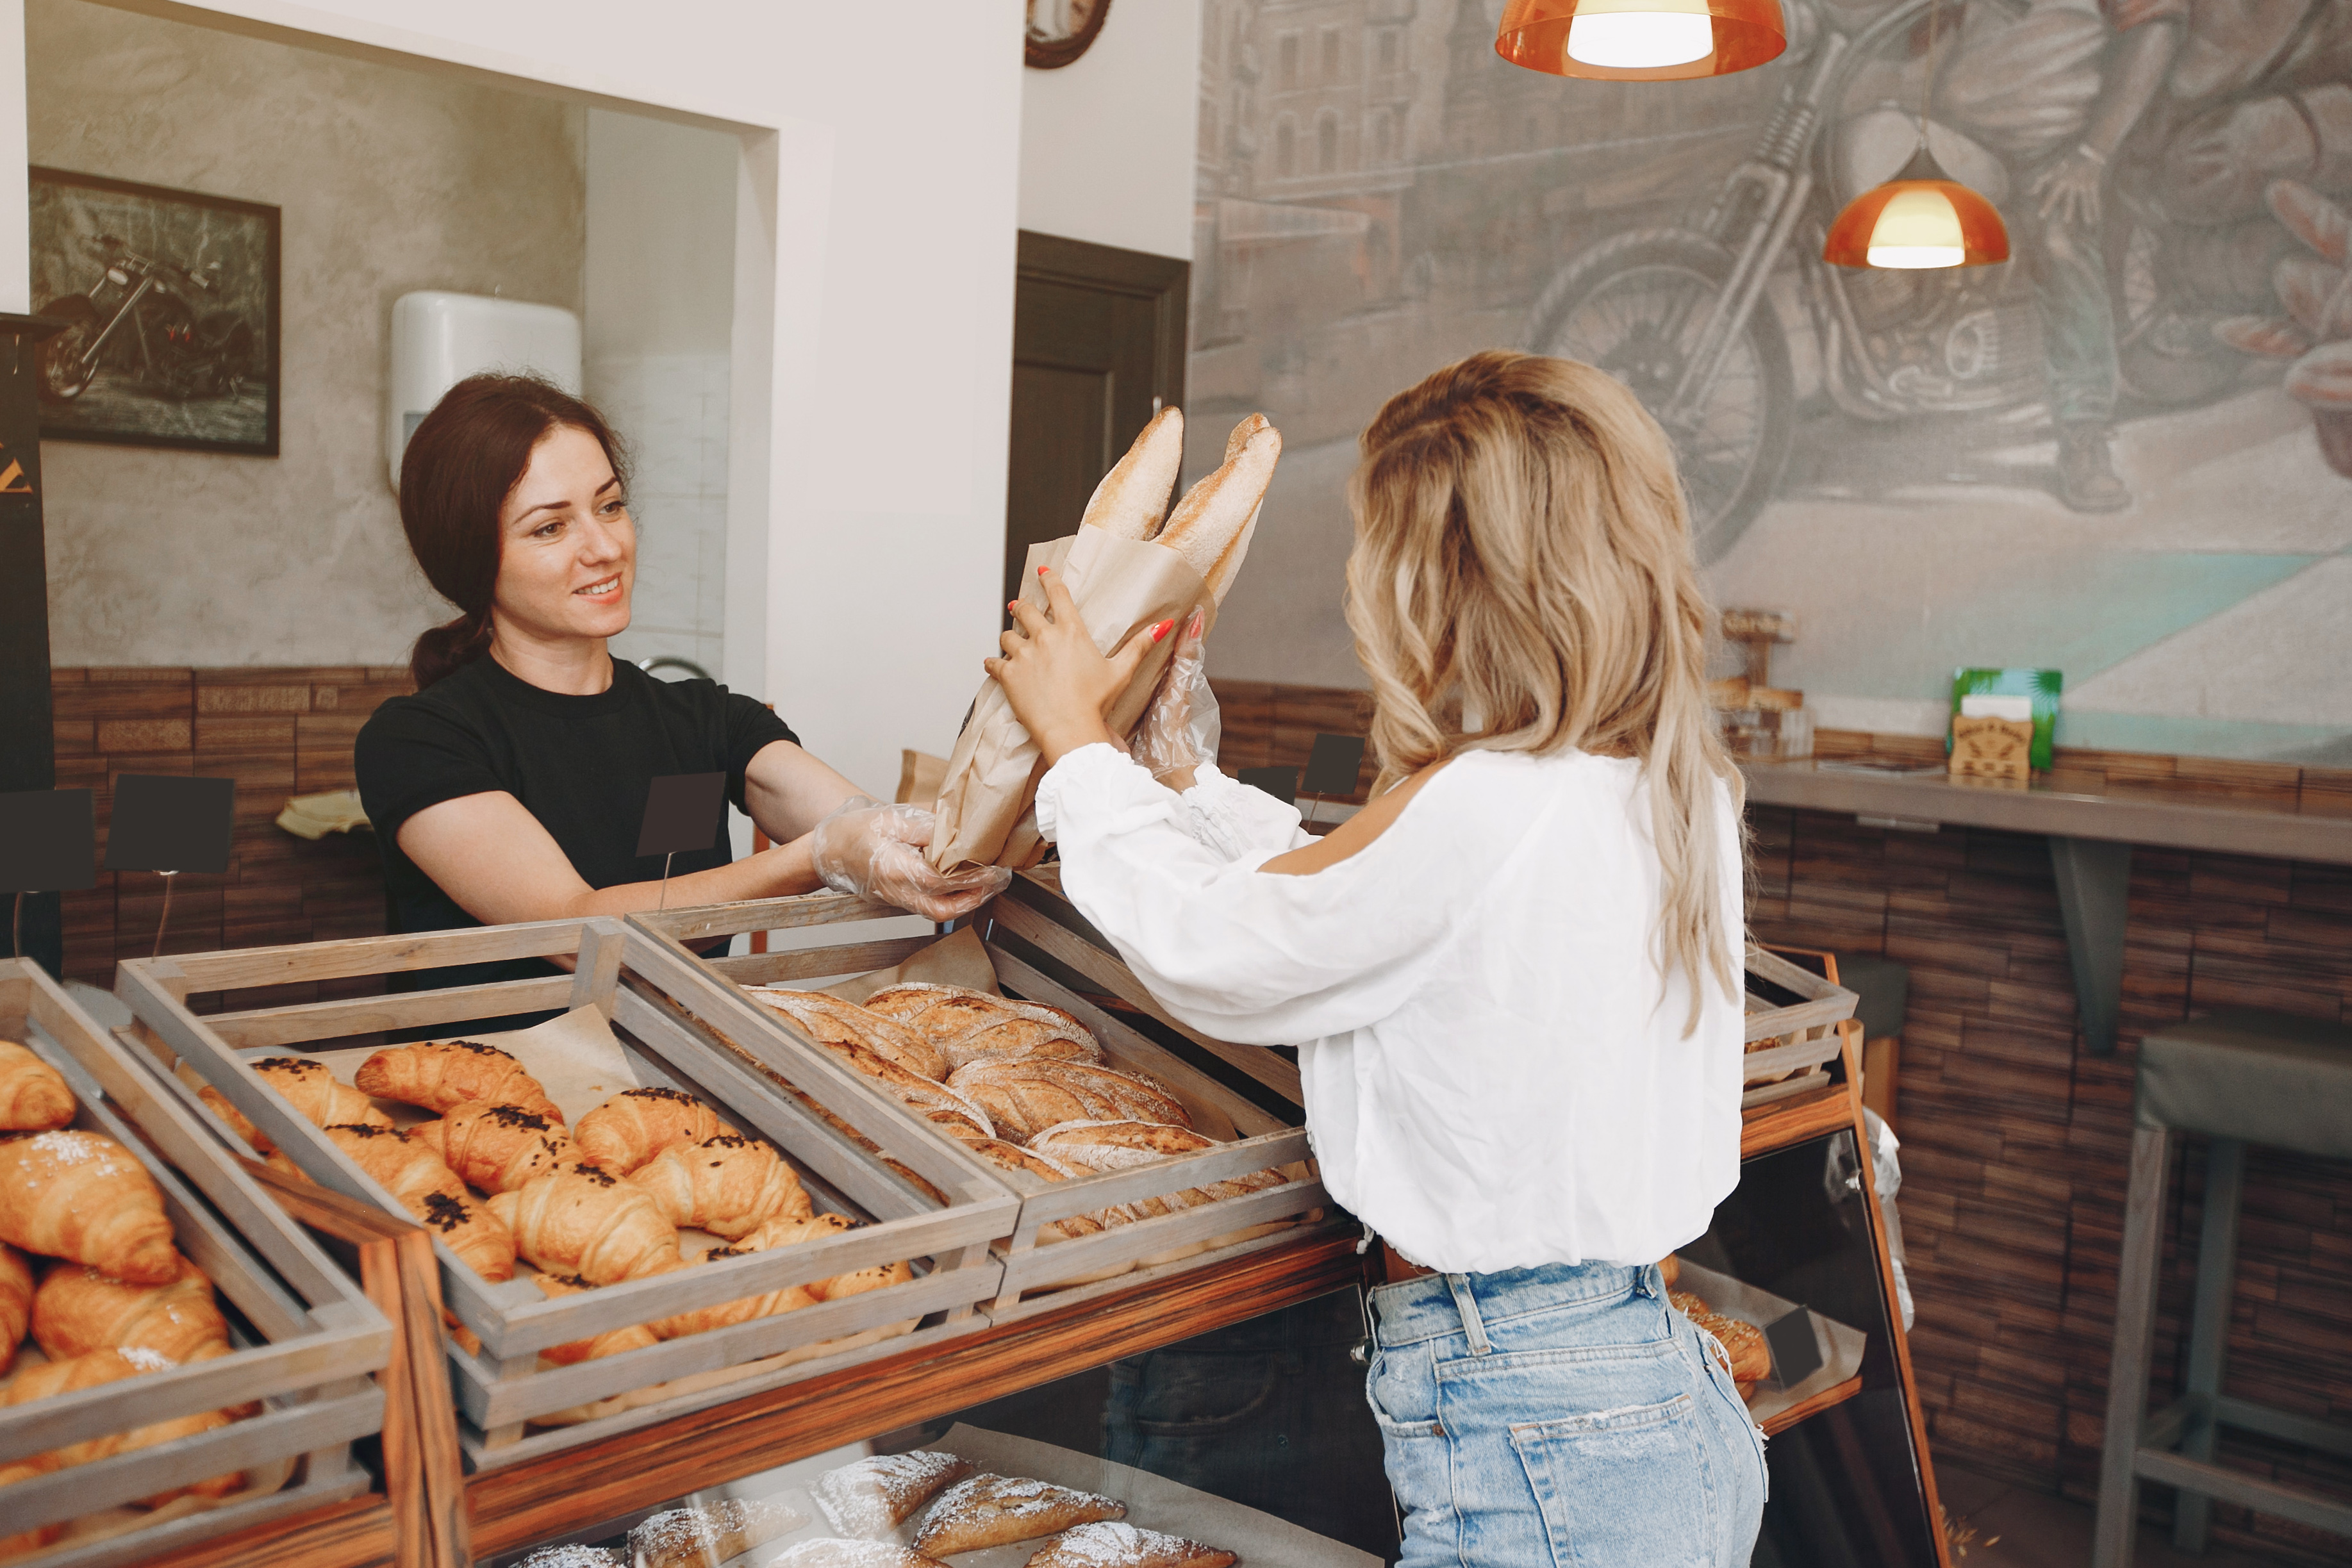
\includegraphics[width=0.7\textwidth]{./imgSAEB_6_POR/freepik/PORT_6_IMG-20.jpeg}
\end{figure}

\begin{quote}
--- Moça, esta baguete é de hoje?
--- Não... é de parmesão.
\end{quote}

\num{1} Na cena, o humor está presente:

\begin{escolha}
\item No fato de a atendente não saber o que é baguete.
\item Na confusão entre a pergunta da cliente e a interpretação da
atendente. 
\item No fato de a atendente não ouvir direito a pergunta.
\item Na simpatia da atendente ao fazer uma piada.
\end{escolha}

% Gabarito, treino?
% \begin{escolha}
% \item Incorreta. Em nenhum momento a tirinha dá a impressão de que a
% atendente não sabe o que é baguete.
% \item Correta. O humor está presente na confusão de interpretações que se fez.
% \item Incorreta. A atendente ouve a pergunta, porém entende-a de forma
% ambígua.
% \item Incorreta. Mesmo que a atendente fizesse uma piada proposital, o
% humor desta residiria no fato de a pergunta ter sido compreendida de forma equivocada.
% \end{escolha}

\num{2} Explique a ambiguidade que poderia ser vista no texto, gerando a
confusão.

\reduline{A ambiguidade está no modo como objeto indireto "de" é usado.
Ao perguntar se a baguete é de hoje, a cliente quer saber se o pão foi
feito naquele dia. Já a atendente entende que ela se referia ao sabor do
pão; então, responde que é de parmesão.\hfill}\linhas{1}

\num{3} Reescreva o texto, de modo a excluir qualquer possibilidade de
confusão na interpretação.

\begin{itemize}[label=$\ast$]
\item \reduline{Moça, essa baguete foi feita hoje?\hfill}
\item \reduline{Sim, foi feita hoje.\hfill}
\item \reduline{E qual é o sabor?\hfill}
\item \reduline{É de parmesão.\hfill}
\end{itemize}

\noindent Leia um trecho de uma crônica de Marina Colasanti e responda às
perguntas de 4 a 6.

\begin{quote}
``Houve um tempo em que comíamos comida. Hoje queremos gastronomia. Nas
casas, {[}\ldots{]} consome-se mais gastronomia na TV {[}\ldots{]}. Mas
na hora de escolher um restaurante, vamos de gastronômicos até onde o
bolso alcança, porque o paladar agradece, e porque gastronomia é moda.''

\fonte{Marina Colasanti. \emph{Bigodões e talheres de ouro}. Disponível em:
https://www.marinacolasanti.com/2015/06/cronica-de-quinta-bigodoes-e-talheres.html.
Acesso em: 10 mar. 2023.}
\end{quote}

\num{4} De acordo com a leitura, qual é a diferença entre comida e
gastronomia?

\reduline{Comida é a forma como as pessoas se referiam ao alimento no
dia a dia, para matar a fome. Com a modernidade, as pessoas não querem
mais apenas comer, querem gastronomia, ou seja, comer de um jeito chique
e, consequentemente, pagando mais.\hfill}\linhas{1}

\num{5} Identifique, no texto, em quais trechos a autora é irônica.

\reduline{Pode-se identificar ironia nas seguintes passagens: "Nas
casas, [\ldots{}] consome-se mais gastronomia na TV [\ldots{}]."; "Mas na hora de escolher um restaurante, vamos de gastronômicos até onde o bolso alcança".\hfill}\linhas{1}

\num{6} Ao dizer que ``nas casas consome-se mais gastronomia na TV'', o
que a autora quer dizer?

\reduline{A autora quer dizer que somos mais seletivos em casa, com o
que escolhemos ver na TV, do que com o que comemos.\hfill}\linhas{1}

\noindent Leia o \textit{post} a seguir, composto de imagem e texto escrito, para resolver
as atividades de 7 a 9.

\begin{figure}[H]
%PORT_6_IMG-21 — POR.tex:2259
\centering\includegraphics[width=0.7\textwidth]{./imgSAEB_6_POR/freepik/PORT_6_IMG-21.jpeg}
\end{figure}

\begin{quote}
Márcia do céu, você não acredita! A almofada explodiu, menina! Veio com
defeito, com certeza\ldots{}
\end{quote}

\num{7} O post é construído com uma cena e contendo apenas uma
personagem: o cachorro. Porém, em seu discurso ele interage com mais
alguém. Quem é essa pessoa e o que ela representa?

\reduline{O cachorro interage com a Márcia, que seria, provavelmente, a dona dele.\hfill}\linhas{1}

\num{8} Quais elementos demonstram que o cão tem uma relação de
proximidade com a Márcia?

\reduline{O fato de o cachorro estar na mesma casa que ela, sentado no
sofá, e o tom informal da fala do cachorro (Márcia do céu; a almofada
explodiu, menina).\hfill}\linhas{1}

\num{9} Explique a ironia contida na cena.

\reduline{O cachorro rasgou toda a almofada, mas justificou contando que
ela havia explodido porque veio com defeito.\hfill}\linhas{1}

\section{Treino}

\num{1} Leia o texto a seguir.

\begin{quote}
\centering\textbf{Afinal, onde está localizado o beleléu?}


\noindent \emph{Passam-se décadas e o tal beleléu continua sendo um enigma para
mim: afinal, onde está localizado o beleléu?}

Ele está no mesmo lugar para onde vão aqueles que partem desta vida.

Essa palavra é um eufemismo utilizado para se referir a morte,
desaparecimento ou perda.

A origem desse termo é obscura, e a hipótese mais aceita é de que seja
uma onomatopeia, ou seja, uma palavra que imita o som produzido.
Acredita-se que beleléu imite o barulho de algo caindo e se estalando no
chão.

\fonte{https://super.abril.com.br/coluna/oraculo/afinal-onde-fica-o-beleleu. Acesso em: 18 mar. 2023.}
\end{quote}

O efeito de humor do texto se encontra no(a):

\begin{escolha}
\item Fato de não se saber o que significa beleléu.
\item Explicação de que é um eufemismo para morte.
\item Fato de beleléu ser uma palavra que imita um som.
\item Fato de a pessoa ficar pensando na palavra beleléu. 
\end{escolha}

%\paragraph{BNCC: EF69LP05} 
% Inferir e justificar, em textos multissemióticos —-
% tirinhas, charges, memes, gifs etc. —, o efeito de humor, ironia e/\,ou
% crítica pelo uso ambíguo de palavras, expressões ou imagens ambíguas, de
% clichês, de recursos iconográficos, de pontuação etc.

% Gabarito, treino?
% \begin{escolha}
% \item Incorreta. A origem do termo é obscura, mas esse é um fato sobre a
% palavra e não o que dá o humor do texto.
% \item Incorreta. O texto explica que é um eufemismo para a morte, mas não é
% isso que provoca o humor.
% \item Incorreta. O fato de ser uma possível onomatopeia não provoca por si
% só o efeito de humor ao texto.
% \item Correta. O efeito de humor é apresentado na linha fina do texto,
% quando a pessoa informa que há décadas fica pensando no ``bendito do
% beleléu''.
% \end{escolha}


\pagebreak
\num{2} Observe o meme, constituído pela foto e pela frase que a
acompanha.

\begin{figure}[H]
%PORT_6_IMG-22 — POR.tex:2341
\centering\includegraphics[width=0.5\textwidth]{./imgSAEB_6_POR/freepik/PORT_6_IMG-22.jpeg}
\end{figure}

\begin{quote}
Já ouvi dizer que elefantes têm boa memória. Mas roupa de post-it faz a
gente parecer mais uma galinha.
\end{quote}

\noindent O efeito de humor do meme emerge:

\begin{escolha}
\item Das feições do homem, que são engraçadas.
\item Do texto verbal, que compara elefantes a galinhas.
\item Da relação entre a foto, que já é engraçada, com o texto, que se
associa a ela. \item Da relação surpreendente entre papéis e animais.
\end{escolha}

%\paragraph{BNCC: EF69LP05} 
% Inferir e justificar, em textos multissemióticos —
% tirinhas, charges, memes, gifs etc. —, o efeito de humor, ironia e/\,ou
% crítica pelo uso ambíguo de palavras, expressões ou imagens ambíguas, de
% clichês, de recursos iconográficos, de pontuação etc.

% Gabarito, treino?
% \begin{escolha}
% \item Incorreta. Apesar de as feições do homem serem de fato engraçadas, o
% humos não emerge disso no meme.
% \item Incorreta. Os dois animais não aparecem em comparação direta.
% \item Correta. A relação entre imagem e texto é o que faz emergir o humor
% do meme.
% \item Incorreta. Essa relação não se estabelece no meme, nem pela imagem,
% nem pelo texto verbal.
% \end{escolha}

\num{3} Observe a campanha publicitária a seguir, composta pela imagem e
pelo texto.

\begin{figure}[H]
%PORT_6_IMG-23 — POR.tex:2375
\centering\includegraphics[width=0.7\textwidth]{./imgSAEB_6_POR/freepik/PORT_6_IMG-23.jpeg}
\end{figure}

\begin{quote}
Quando o assunto é delicadeza, não adianta colocar adereço por fora; é
de dentro que ela vem. Seja educado. Ofereça lugar no transporte público
para aqueles que realmente precisam. \%se for possível, aplicar a frase
sobre a parte de fundo rosa da imagem.
\end{quote}

O que explica o efeito de humor da publicidade é:

\begin{escolha}
\item a ironia presente no texto.
\item o uso do verbo no imperativo.
\item o improvável da imagem, especialmente quando ela se conjuga com o
texto verbal. \item a relação equivocada entre a cor rosa e a educação no trânsito,
geralmente ligada à cor amarela.
\end{escolha}

%\paragraph{BNCC: EF69LP05} 
% Inferir e justificar, em textos multissemióticos --
% tirinhas, charges, memes, gifs etc. --, o efeito de humor, ironia e/\,ou
% crítica pelo uso ambíguo de palavras, expressões ou imagens ambíguas, de
% clichês, de recursos iconográficos, de pontuação etc.

% Gabarito, treino?
% \begin{escolha}
% \item Incorreta. Não há ironia no texto verbal.
% \item Incorreta. O verbo no imperativo, pelo contrário, faz uma referência
% direta ao leitor, pedindo uma atitude realmente útil.
% \item Correta. O homem forte vestido de fada e a relação da imagem dele com
% o texto verbal é o que gera humor.
% \item Incorreta. De fato, a cor amarela é ligada à educação no trânsito.
% Mas não há equívoco proposital no uso da cor rosa nesse caso.
% \end{escolha}

\chapter{Tudo o que se lê é verdade?}
\markboth{Módulo 7}{}

\section{Habilidades do SAEB}
\begin{itemize}
\item Analisar marcas de parcialidade em textos
jornalísticos. 
\item Avaliar diferentes graus de parcialidade em textos
jornalísticos. 
\item Avaliar a fidedignidade de informações sobre um mesmo
fato divulgado em diferentes veículos e mídias.
\end{itemize}

\subsection{Habilidades da BNCC}
\begin{itemize}
\item EF06LP01
\item EF67LP03
\item EF67LP04
\end{itemize}

\conteudo{
Uma notícia é um relato factual de um evento, acontecimento ou situação
que se considera de interesse público. A notícia é geralmente divulgada
pelos meios de comunicação, como jornais, revistas, *sites* de notícias,
rádio e televisão, com o objetivo de informar o público sobre os
acontecimentos relevantes que afetam a sociedade.

As principais características de uma notícia incluem:}

\conteudo{
\paragraph{Atualidade} recente e atual, relata algo que acabou de acontecer ou
foi descoberto.

\paragraph{Objetividade} apresentada de forma imparcial, sem opiniões pessoais
ou julgamentos de valor.

\paragraph{Clareza} necessita ser escrita de forma clara e concisa, usando uma
linguagem simples e direta para que o leitor possa compreender
facilmente.

\paragraph{Relevância} deve ser de interesse público e ter uma importância
significativa para a sociedade.

\paragraph{Precisão} A notícia deve ser precisa e baseada em fatos
verificáveis, com informações precisas e corretas.

\paragraph{Novidade} A notícia deve ter algo de novo ou original que chame a
atenção do leitor ou ouvinte.

\paragraph{Conexão} deve estabelecer uma conexão com o público,
identificando-se com seus interesses e necessidades.

{}Existem diversos gêneros textuais jornalísticos, além das notícias e reportagens. Abaixo estão alguns dos principais.{}

\paragraph{Notícia} é o gênero mais comum do jornalismo e se refere a um relato
breve e objetivo sobre um fato atual, importante e de interesse público.

\paragraph{Reportagem} é uma forma mais elaborada de notícia, que traz mais
informações e detalhes sobre um assunto. Pode ser dividida em reportagem
especial, investigativa, interpretativa, entre outras.

\paragraph{Editorial} é um texto opinativo, escrito pelo editor-chefe ou por um
colunista, que expressa a opinião do veículo de comunicação sobre um
assunto.

\paragraph{Entrevista} é uma conversa entre o jornalista e uma pessoa ou grupo
de pessoas, com o objetivo de obter informações e opiniões sobre um tema
específico.

\paragraph{Artigo} é um texto opinativo, escrito por um colunista ou
especialista, que apresenta argumentos e reflexões sobre um assunto.

\paragraph{Crônica} é um texto que mistura fatos e ficção, que trata de
assuntos cotidianos e que busca entreter o leitor.

\paragraph{Resenha} é uma análise crítica sobre um livro, filme, peça de teatro
ou outro tipo de obra.

\paragraph{Nota} é um texto curto e objetivo, que traz uma informação rápida
sobre um acontecimento de menor importância.

\paragraph{Editorial de seção} é um texto opinativo sobre um tema específico,
escrito pelo editor-chefe ou por um colunista, que é publicado
regularmente em uma determinada seção do veículo de comunicação.

\paragraph{Infográfico} é uma representação gráfica que combina texto, imagem e
outros elementos visuais para apresentar informações de forma clara e
concisa.}

\conteudo{
A parcialidade e a imparcialidade são duas abordagens diferentes que os
jornalistas podem adotar na produção de textos jornalísticos.

A \textbf{imparcialidade} busca apresentar as informações de forma objetiva e
sem opiniões pessoais e é geralmente vista como uma característica
importante do jornalismo profissional e ético. O jornalista imparcial
deve se manter neutro e evitar tomar partido em qualquer questão. Nesse
tipo de abordagem, o objetivo principal é transmitir informações
precisas e confiáveis aos leitores, para que possam tirar suas próprias
conclusões.

Já a \textbf{parcialidade} é uma abordagem que envolve a inclusão de opiniões
pessoais do jornalista em um texto jornalístico. Nesse caso, o objetivo
é expressar uma visão pessoal sobre um determinado assunto e influenciar
a opinião dos leitores. Essa abordagem pode ser usada em editoriais,
colunas de opinião e outras formas de jornalismo interpretativo.

É importante ressaltar que a parcialidade não é necessariamente ruim ou
antiética. No entanto, os jornalistas que adotam essa abordagem devem
deixar claro que estão expressando sua opinião pessoal e não
apresentando um fato objetivo. A transparência é essencial para que os
leitores possam entender a perspectiva do jornalista e decidir se
concordam ou não com a opinião apresentada.

De maneira geral, o objetivo do jornalismo é fornecer informações
precisas e confiáveis aos leitores, independentemente da abordagem
adotada pelo jornalista. No entanto, é importante que o leitor possa
distinguir entre fatos objetivos e opiniões pessoais, para que possa
formar sua própria opinião com base em informações precisas e
confiáveis.

Lembre-se de que nem todos os textos são completamente verdadeiros ou
completamente falsos. É importante ler com atenção, analisar
criticamente e considerar várias fontes para chegar a uma conclusão
informada.}

\conteudo{
Há vários fatores que podem ajudar a determinar a veracidade de um
texto, como:

\paragraph{Fonte} uma fonte confiável é aquela que tem uma reputação
sólida por fornecer informações precisas e imparciais. Verifique se o
autor do texto é uma fonte confiável ou se está baseando suas
informações em fontes confiáveis.

\paragraph{Evidências} um texto que apresenta evidências sólidas para apoiar suas
afirmações é mais provável de ser verdadeiro. As evidências podem ser
dados estatísticos, citações de especialistas, referências a pesquisas
científicas, entre outros.

\paragraph{Consistência} verifique se as informações apresentadas no texto são
consistentes com outras fontes confiáveis. Se outras fontes confiáveis
também confirmam as informações, isso aumenta a probabilidade de que
elas sejam verdadeiras.

\paragraph{Linguagem} observe se o texto utiliza uma linguagem precisa e objetiva.
Textos que usam uma linguagem vaga ou ambígua podem indicar que o autor
está tentando enganar ou manipular o leitor.

\paragraph{Motivação} verifique se o autor do texto tem alguma motivação para
enganar ou manipular o leitor. Por exemplo, se o autor é um político que
está tentando obter votos, ele pode distorcer a verdade para atingir
seus objetivos.}


\section{Atividades}

\noindent Leia as três manchetes a seguir, inspiradas em outras encontradas na
internet, para resolver as atividades de 1 a 10.

\begin{quote}
\textbf{Texto I}\\
\medskip

\noindent\textbf{Netflix quer acabar com farra de compartilhamento de senhas;
será em 2023}\\
\emph{A Netflix lançou um ultimato para quem divide sua
senha do serviço com amigos e parentes. A ``farra'' deve terminar no
próximo ano.} 

\fonte{Data: 19 out. de 2022.}
\end{quote}

\begin{quote}
\textbf{Texto II}\\
\medskip

\noindent\textbf{Plataforma Netflix anuncia regras atualizadas sobre o
compartilhamento de senhas}\\
\emph{Compartilhamento é prática irregular,
proibida nos contratos dos serviços de streaming. Em 2021, realizou-se
um teste\ldots{}} 

\fonte{Data: 1 mês atrás.}
\end{quote}

\begin{quote}
\textbf{Texto III}\\
\medskip

\noindent\textbf{Sim, Netflix cobrará mais de quem divide senha; veja regras}
\emph{A Netflix lançou um ultimato para quem divide sua senha do serviço
com amigos e parentes. A ``farra'' deve terminar em 2023.} 

\fonte{Data: 19 de out. 2022.}
\end{quote}

\num{1} Qual é a temática comum entre as manchetes?

\reduline{O compartilhamento de senhas na Netflix.\hfill}\linhas{1}

\num{2} Qual das três manchetes apresenta um texto com informações mais
claras e objetivas relacionadas ao tema?

\reduline{A manchete do texto 2.\hfill}\linhas{1}

\num{3} É possível saber qual das três manchetes apresenta a notícia
mais recente? Justifique sua resposta.

\reduline{Não é possível saber, pois o texto 2 apresenta a data de "um
mês atrás", e não se sabe a qual mês ele se refere.\hfill}\linhas{1}

\num{4} O texto 1 e o texto 3, divulgados na mesma página, apresentam
semelhanças e diferenças. Qual das duas manchetes fornece dados mais
confiáveis ao leitor? Por quê?

\reduline{A manchete do texto 3 apresenta informações que geram mais
confiança, pois além de ter uma linguagem mais formal, no título ela já
anuncia que há regras para o compartilhamento de senhas.\hfill}\linhas{1}

\num{5} Qual das manchetes apresenta viés de opinião pessoal? Em quais
trechos é possível identificar isso?

\reduline{Na manchete do texto 1. O autor da notícia se refere ao
compartilhamento de senhas como "farra". Isso dá ao leitor a impressão
de que o compartilhamento de senhas é uma festa, uma diversão para o
usuário da Netflix. No subtítulo da matéria, ele também informa que as
pessoas compartilhas senhas com amigos e parentes, dando a entender que
sabe de que maneira essa prática funciona.\hfill}\linhas{1}

\num{6} Nos três textos o leitor pode inferir que a prática de
compartilhar senhas é errada. Em qual deles isso é trazido como uma
certeza? Em que trecho é possível identificar essa informação?

\reduline{No texto 2. O subtítulo da manchete apresenta a informação de
que a prática é irregular e vedada em contrato.\hfill}\linhas{1}

\num{7} No texto 3, a manchete apresentada inicia-se com :
``\textbf{Sim}, Netflix vai cobrar mais de quem divide senha em 2023''.
Que efeito de sentido essa escolha lexical provoca no leitor?

\reduline{O "Sim" afirma ao leitor que a notícia é de fato verdadeira,
que foi conferida, ou seja, que a Netflix vai mesmo cobrar pelo
compartilhamento de senhas.\hfill}\linhas{1}

\num{8} No texto 3, qual termo é utilizado para informar que o
compartilhamento de senhas é uma prática irregular?

\reduline{O termo utilizado é ``combater''.\hfill}\linhas{1}

\num{9} Considerando as informações apresentadas nas manchetes e linhas
finas dos três textos, redija uma manchete e uma linha fina que
apresente informações precisas para o leitor ser qualquer viés de
opinião.

\reduline{Embora aqui a resposta seja de certa forma
pessoal para os alunos, espera-se que todos abordem, na manchete, o tema
principal da notícia, comum entre os três textos, e na linha fina uma
breve explicação do contexto. Segue exemplo: \textbf{Netflix anuncia novas regras para o compartilhamento de senhas}: Usuários terão que pagar caso desejem continuar com a prática.\hfill}\linhas{1}

\num{10} Ao abrir essas notícias, para quais dados o leitor deve se
atentar a fim de saber se as informações foram checadas antes de ser
publicadas?

\reduline{A linguagem utilizada na notícia, sem viés de opinião; a data
de publicação da notícia; se o veículo que a publicou é de
credibilidade; se o texto apresenta uma referência bibliográfica para
a fonte das informações.\hfill}\linhas{1}

\section{Treino}

\num{1} Leia o texto a seguir.

\begin{figure}[H]
%PORT_6_IMG-24 — POR.tex:2685
\centering\includegraphics[width=0.7\textwidth]{./imgSAEB_6_POR/freepik/PORT_6_IMG-24.jpeg}
\end{figure}

\begin{quote}
\centering\textbf{Tratar animal de estimação como filho, ser ``pai de pet'' faz mal à saúde mental?}\\
\medskip


\noindent Aqueles que amam e cuidam adequadamente de animais de estimação buscam
proporcionar o melhor para eles, pois esses animais são considerados
parte da família por muitas pessoas. No entanto, não é saudável nem
recomendado tratar um cão ou gato como se fossem seres humanos, nem
esperar que se comportem como crianças pequenas. Isso ocorre porque,
além de prejudicá-los - afinal, eles pertencem a diferentes espécies e
possuem seus próprios instintos e comportamentos - essa abordagem também
pode ser prejudicial para os tutores.

É verdade que sentimentos positivos contribuem para a saúde humana, mas
é importante que prestemos atenção ao nosso entorno e direcionemos essa
dedicação também para outras áreas de nossas vidas que merecem cuidado.
Quando isso não acontece e o foco se concentra exclusivamente nos
animais, pode ser que a pessoa inconscientemente esteja tentando
satisfazer um forte desejo, como o de ter filhos, ou procurando
relacionamentos e emoções, mas não é capaz ou enfrenta dificuldades para
interagir e aceitar críticas.

\fonte{Marcelo Testoni. Uol. \emph{``Pai de pet'': faz mal à saúde mental tratar
animal de estimação como filho?} Disponível em: www.uol.com.br/vivabem/noticias/redacao/2021/03/10/animal-de-estimacao-como-filho.htm. Acesso em: mar. 2023. Adaptado.}
\end{quote}

Assinale a alternativa correta sobre a escolha do título do texto.

\begin{escolha}
\item A resposta à pergunta do título é dada a partir do ponto de vista do
autor do texto.
\item A pergunta no título tem o intuito de gerar uma reflexão no leitor do
texto.
\item Apresenta um viés pejorativo, o que pode ser comprovado pelo uso de
aspas.
\item Traz uma pergunta de senso comum, já que muitas pessoas tratam
animais como filhos. 
\end{escolha}

%\paragraph{BNCC: EF67LP04} 
% Distinguir, em segmentos descontínuos de textos, fato
% da opinião enunciada em relação a esse mesmo fato.

% Gabarito, treino?
% \begin{escolha}
% \item Incorreta. A resposta, dada no primeiro parágrafo, não é a opinião do
% autor, e sim uma explicação técnica.
% \item Incorreta. A pergunta é assertiva é não tem o intuito de gerar
% reflexão, uma vez que a resposta já é fornecida no primeiro parágrafo.
% \item Incorreta. A expressão está entre aspas porque ``pai de pet'' é um
% termo comum apenas a pessoas que o conhecem.
% \item Correta. O título é uma pergunta pertinente e de senso comum, pois
% muitas pessoas consideram pets como filhos.
% \end{escolha}

\num{2} Observe os dois títulos a seguir, inspirados em manchetes da
internet.

\begin{figure}[H]
%PORT_6_IMG-25 — POR.tex:2742
\centering\includegraphics[width=0.7\textwidth]{./imgSAEB_6_POR/freepik/PORT_6_IMG-25.jpeg}
\end{figure}

\begin{quote}
\noindent\textbf{Título 1}\quad Ser ``pai de pet'' faz mal à saúde mental?

\noindent\textbf{Título 2}\quad Como é a vida e como é a rotina de um pai de pet: especialmente no dia
dos pais.
\end{quote}

\begin{escolha}
\item Ambos os títulos apresentam o ponto de vista do veículo.
\item Somente o Título 2 apresenta o ponto de vista do veículo. 
\item Somente o Título 1 apresenta o ponto de vista do veículo.
\item Nenhum dos títulos apresenta o ponto de vista do veículo.
\end{escolha}

%\paragraph{BNCC: EF67LP03} 
% Comparar informações sobre um mesmo fato divulgadas em
% diferentes veículos e mídias, analisando e avaliando a confiabilidade.

% Gabarito, treino?
% \begin{escolha}
% \item Incorreta. Apenas o Título 2 apresenta o ponto de vista do veículo.
% \item Correta. O Título 2 apresenta o ponto de vista do veículo ao
% confirmar que pessoas são pais de pet, admitindo que há uma rotina para
% essas pessoas.
% \item Incorreta. O Título 1 apresenta o tema da matéria por meio de uma
% pergunta, sem se posicionar a respeito dela.
% \item Incorreta. O Título 2 apresenta sim um ponto de vista a respeito do
% tema da matéria.
% \end{escolha}

\num{3} Leia o texto a seguir.

\begin{figure}[H]
%PORT_6_IMG-26 — POR.tex:2786
\centering\includegraphics[width=0.7\textwidth]{./imgSAEB_6_POR/freepik/PORT_6_IMG-26.jpeg}
\end{figure}

\begin{quote}
\emph{Nova Iorque/Genebra, Brasília, 10 de junho de 2021.} O número de
crianças e adolescentes envolvidos em trabalho infantil atingiu a marca
de 160 milhões em todo o mundo. Esse número representa um aumento de 8,4
milhões de meninos e meninas nos últimos quatro anos, de 2016 a 2020.
Além disso, há outros 8,9 milhões de crianças em risco de entrar nessa
situação até 2022, devido aos impactos da pandemia da Covid-19. Esses
dados são apresentados em um novo relatório divulgado pela Organização
Internacional do Trabalho (OIT) e pelo Fundo das Nações Unidas para a
Infância (UNICEF).

O diretor-geral da OIT, Guy Ryder, destacou a importância dessas
estimativas, ressaltando que não podemos ficar inertes enquanto uma nova
geração de crianças é exposta a esses riscos.

\fonte{UNICEF. \emph{Trabalho infantil aumenta pela primeira vez em duas décadas e atinge um total de 160 milhões de crianças e adolescentes no mundo}. Disponível em: https://www.unicef.org/brazil/comunicados-de-imprensa/trabalho-infantil-aumenta-pela-primeira-vez-em-duas-decadas-e-atinge-um-total-de-160-milhoes-de-criancas-e-adolescentes-no-mundo. Acesso em: mar. 2023. Adaptado.}
\end{quote}

\noindent O trecho que reapresenta um ponto de vista é:

\begin{escolha}
\item ``Há outros 8,9 milhões de crianças em risco de entrar nessa situação
até 2022''.
\item ``Esses dados são apresentados em um novo relatório divulgado pela
Organização Internacional do Trabalho''.
\item ``O diretor-geral da OIT, Guy Ryder, destacou a importância dessas
estimativas''.
\item ``Não podemos ficar inertes''.
\end{escolha}

%\paragraph{BNCC: EF67LP03} 
% Comparar informações sobre um mesmo fato divulgadas em
% diferentes veículos e mídias, analisando e avaliando a confiabilidade.

% Gabarito, treino?
% \begin{escolha}
% \item Incorreta. O trecho apresenta uma possibilidade real de acontecer,
% mediante um fato apresentado.
% \item Incorreta. O trecho apresenta um fato constatado após um a pesquisa.
% \item Incorreta. Trata-se de um fato que Guy Ryder é diretor-geral da OIT e
% que ele destacou esse ponto sobre os dados.
% \item Correta. É um posicionamento do diretor-geral da OIT que não podemos
% ficar parados diante dos dados apresentados sobre o trabalho infantil.
% \end{escolha}


\chapter{Os modalizadores do discurso em nosso dia a dia}
\markboth{Módulo 8}{}

\section{Habilidades do SAEB}
\begin{itemize}
\item Identificar os recursos de modalização em textos
diversos. 
\item Analisar os efeitos de sentido dos tempos, modos e/\,ou vozes
verbais com base no gênero textual e na intenção comunicativa. -
Analisar os efeitos de sentido produzidos pelo uso de modalizadores em
textos diversos.
\end{itemize}

\subsection{Habilidades da BNC}
\begin{itemize}
\item EF69LP04 
\item EF69LP28
\end{itemize}

\conteudo{
O modalizador é uma palavra ou expressão por meio de que o enunciador
revela seu posicionamento em uma situação comunicativa. De forma
implícita ou explícita, em textos de impacto social é frequente que os
posicionamentos das pessoas fiquem subentendidos, influenciando o leitor
a compreender o que é dito por ele. Em outras palavras, o modalizador
modifica a maneira de como dizemos/\,escrevemos as ideias.

Podem ser empregados como modalizadores adjetivos, advérbios, modos
verbais como o imperativo, locuções verbais etc.}

\section{Atividades}

\num{1} Leia as frases a seguir e classifique o posicionamento do
enunciador quanto à \textbf{possibilidade}, \textbf{certeza} ou
\textbf{obrigatoriedade}.

\begin{escolha}
\item É indiscutivelmente possível viajar para qualquer lugar do mundo
tendo bastante dinheiro. \reduline{Certeza.\hfill}
\item Peça para sua mãe deixar você dormir na minha casa. \reduline{Obrigatoriedade/\,possibilidade.\hfill}
\item Talvez eu vá ao jogo sexta-feira. \reduline{Possibilidade.\hfill}
\item Compre em até 10x sem juros. \reduline{obrigatoriedade/\,Possibilidade.\hfill}
\item Não tenho certeza se vou à festa
amanhã. \reduline{Possibilidade.\hfill}
\item Se eu conseguir chegar a tempo, vou à sua casa ainda
hoje. \reduline{Possibilidade.\hfill}
\item É proibido fumar neste lugar. \reduline{Certeza.\hfill}
\item Não é permitido entrar com animais neste
estabelecimento. \reduline{Certeza.\hfill}
\end{escolha}

\noindent Leia a resenha crítica do filme \emph{Yesterday} para responder às questões
de 2 a 7.


\begin{quote}
E se em um universo alternativo os Beatles nunca tivessem existido? Se
John, Paul, George e Ringo nunca tivessem criado a maior banda de todos
os tempos? Pois é a partir dessa premissa que caminha \emph{Yesterday},
de Danny Boyle. E enveredamos pela mais pura fantasia, um quase realismo
mágico, se quiserem.

A história é um tanto simplista, mas tem sua beleza. Um músico amador,
vivido por Himesh Patel, em busca do sucesso (clichê, mas aceitável) e
que vive no interior da Inglaterra sofre um acidente quando sua
bicicleta é atropelada no exato momento em que o mundo todo sofre um
apagão. Explosões solares, explica-se a seguir. Mas isso é o que menos
importa. Quando acorda, no hospital, Jack Malik (coincidência ou não, o
mesmo sobrenome do Jamal de \emph{Quem Quer Ser Um Milionário}), está
sem dois dentes, com o violão e a bicicleta quebrados e em um mundo
muito estranho. Porque ninguém nunca ouviu falar dos Beatles. Só para
constar: somem do mapa também a Coca-Cola e o cigarro. Mas isso não faz
diferença. {[}\ldots{}{]}

Entre canções assobiáveis há décadas, desencontros e encontros
improváveis, mas tocantes — a vontade de dar \emph{spoiler} aqui se
torna quase incontornável —, o filme caminha na forma clássica das
comédias românticas, algo que embala, diverte e rende conversas animadas
no pós-crédito. Mas fica a pergunta: e se os Beatles nunca tivessem, de
fato, existido? A resposta vem de uma frase dita quase no final do
filme: ``Um mundo sem os Beatles seria um mundo muito pior''. Não
precisamos disso.

\fonte{Marcello Rollember. Jornal da UPS. ``Para tempos sombrios, a solução é a
fantasia''. Disponível em: https://jornal.usp.br/cultura/para-tempos-sombrios-a-solucao-e-a-fantasia. Acesso em: mar. 2023.}
\end{quote}

\num{2} No primeiro parágrafo do texto, o autor utiliza como modalizador
do discurso uma mesma conjunção, porém em algumas ocorrências distintas.
Qual é esse modalizador e que intenção ele representa?

\reduline{O modalizador utilizado é a conjunção "se", que, em todas as
ocorrências do parágrafo, indicam uma condição.\hfill}\linhas{1}

\num{3} No segundo parágrafo, o autor da resenha crítica apresenta sua
opinião sobre a história. Em qual trecho isso aparece e qual termo ele
utiliza para fazer um julgamento de valor?

\reduline{O trecho em que ele deixa claro seu posicionamento é "A
história é um tanto simplista, mas tem sua beleza.". O termo que ele
utiliza para deixar explícito esse julgamento de valor é o adjetivo
"simplista".\hfill}\linhas{1}

\num{4} Ainda no segundo parágrafo, no trecho ``clichê, mas aceitável'',
ele demostra outro julgamento de valor. A que ele se refere?

\reduline{Ele se refere ao fato de a personagem ser um músico amador em
busca do sucesso.\hfill}\linhas{1}

\num{5} No segundo parágrafo, o resenhista informa que o músico da
história acorda no hospital ``em um mundo \textbf{muito estranho}''.
Isso é uma opinião do autor ou uma verdade que aparece no filme? O que
justifica a escolha desse adjetivo pelo autor?

\reduline{Isso é uma opinião do autor, porque, para ele, é muito
estranho um mundo em que as pessoas não conheçam os Beatles.\hfill}\linhas{1}

\num{6} Releia o início do terceiro parágrafo do texto:

\begin{quote}
Entre canções assobiáveis há décadas, desencontros e encontros
improváveis, mas tocantes — a vontade de dar \emph{spoiler} aqui se
torna quase incontornável —, o filme caminha na forma clássica das
comédias românticas, algo que embala, diverte e rende conversas animadas
no pós-crédito.
\end{quote}

\noindent Identifique, neste trecho, o que são fatos apresentados no filme e o que
é opinião do autor.

\reduline{
  \textbf{Fatos do filme:} Apresenta canções conhecidas, desencontros e encontros improváveis, filme que caminha na forma clássica das comédias românticas, filme que embala, diverte e rende conversas no pós-crédito. \textbf{Opinião do autor:} Canções assobiáveis há décadas, encontros e desencontros improváveis, mas tocantes; vontade de dar spoiler quase incontornável; o filme rende conversas animadas no pós-crédito.\hfill}\linhas{1}

\num{7} Analise as frases extraídas do texto. Depois, analise o
modalizador em destaque e classifique-o quanto a ser uma condição ou uma
certeza.

\begin{escolha}
\item Mas fica a pergunta: e \textbf{{se}} os Beatles nunca tivessem,
\textbf{{de fato}}, existido? \reduline{Se = condição; de fato = certeza.\hfill}
\item Um músico amador, que vive no interior da Inglaterra, sofre um
acidente quando sua bicicleta é atropelada no \textbf{{exato}} momento
em que o mundo todo sofre um apagão. {Exato = certeza.\hfill}
\item A vontade de dar \emph{spoiler} se torna \textbf{{quase}}
\textbf{{incontornável}}. \reduline{Quase = condição; incontornável = certeza.\hfill}
\item \textbf{{Não precisamos}} disso. \reduline{Não precisamos = certeza.\hfill}
\end{escolha}

\noindent Veja a campanha de incentivo à leitura, a seguir, composta de imagem e
de texto verbal, para responder às questões de 8 a 10.

\begin{figure}[H]
\centering
\includegraphics[width=2.14842in,height=3.03846in]{./imgSAEB_6_POR/media/image25.jpeg}
\caption{Diagrama Descrição gerada automaticamente}
\end{figure}

\fonte{\url{https://torres.rs.gov.br/2018/07/27/vem-ai-o-projeto-esqueca-um-livro-com-o-proposito-de-incentivar-a-leitura/}}

\num{8} O tempo verbal predominante na campanha é o imperativo
afirmativo. Qual é a intenção comunicativa do texto?

\reduline{A intenção é convencer o leitor a adotar a ideia da campanha,
que é esquecer um livro em lugares públicos.\hfill}\linhas{1}

\num{9} A palavra ``realizada'' qualifica um termo que a precede. Que
termo é esse?\EP[1]

\reduline{O termo é "ação".\hfill}\linhas{1}

\num{10} Analise a frase a seguir.

\begin{quote}
Uma ação realizada por voluntários de \textbf{{todo}} o Brasil.
\end{quote}

\noindent Qual é o objetivo do uso desse modalizador nesta frase?

\reduline{O objetivo é reforçar, afirmar, que pessoas do Brasil inteiro
estão aderindo à campanha.\hfill}\linhas{1}

\section{Treino}

\num{1} Observe a imagem de uma campanha contra o bullying e leia o
texto que a acompanha.

\begin{figure}[H]
%PORT_6_IMG-27 — POR.tex:3057
\centering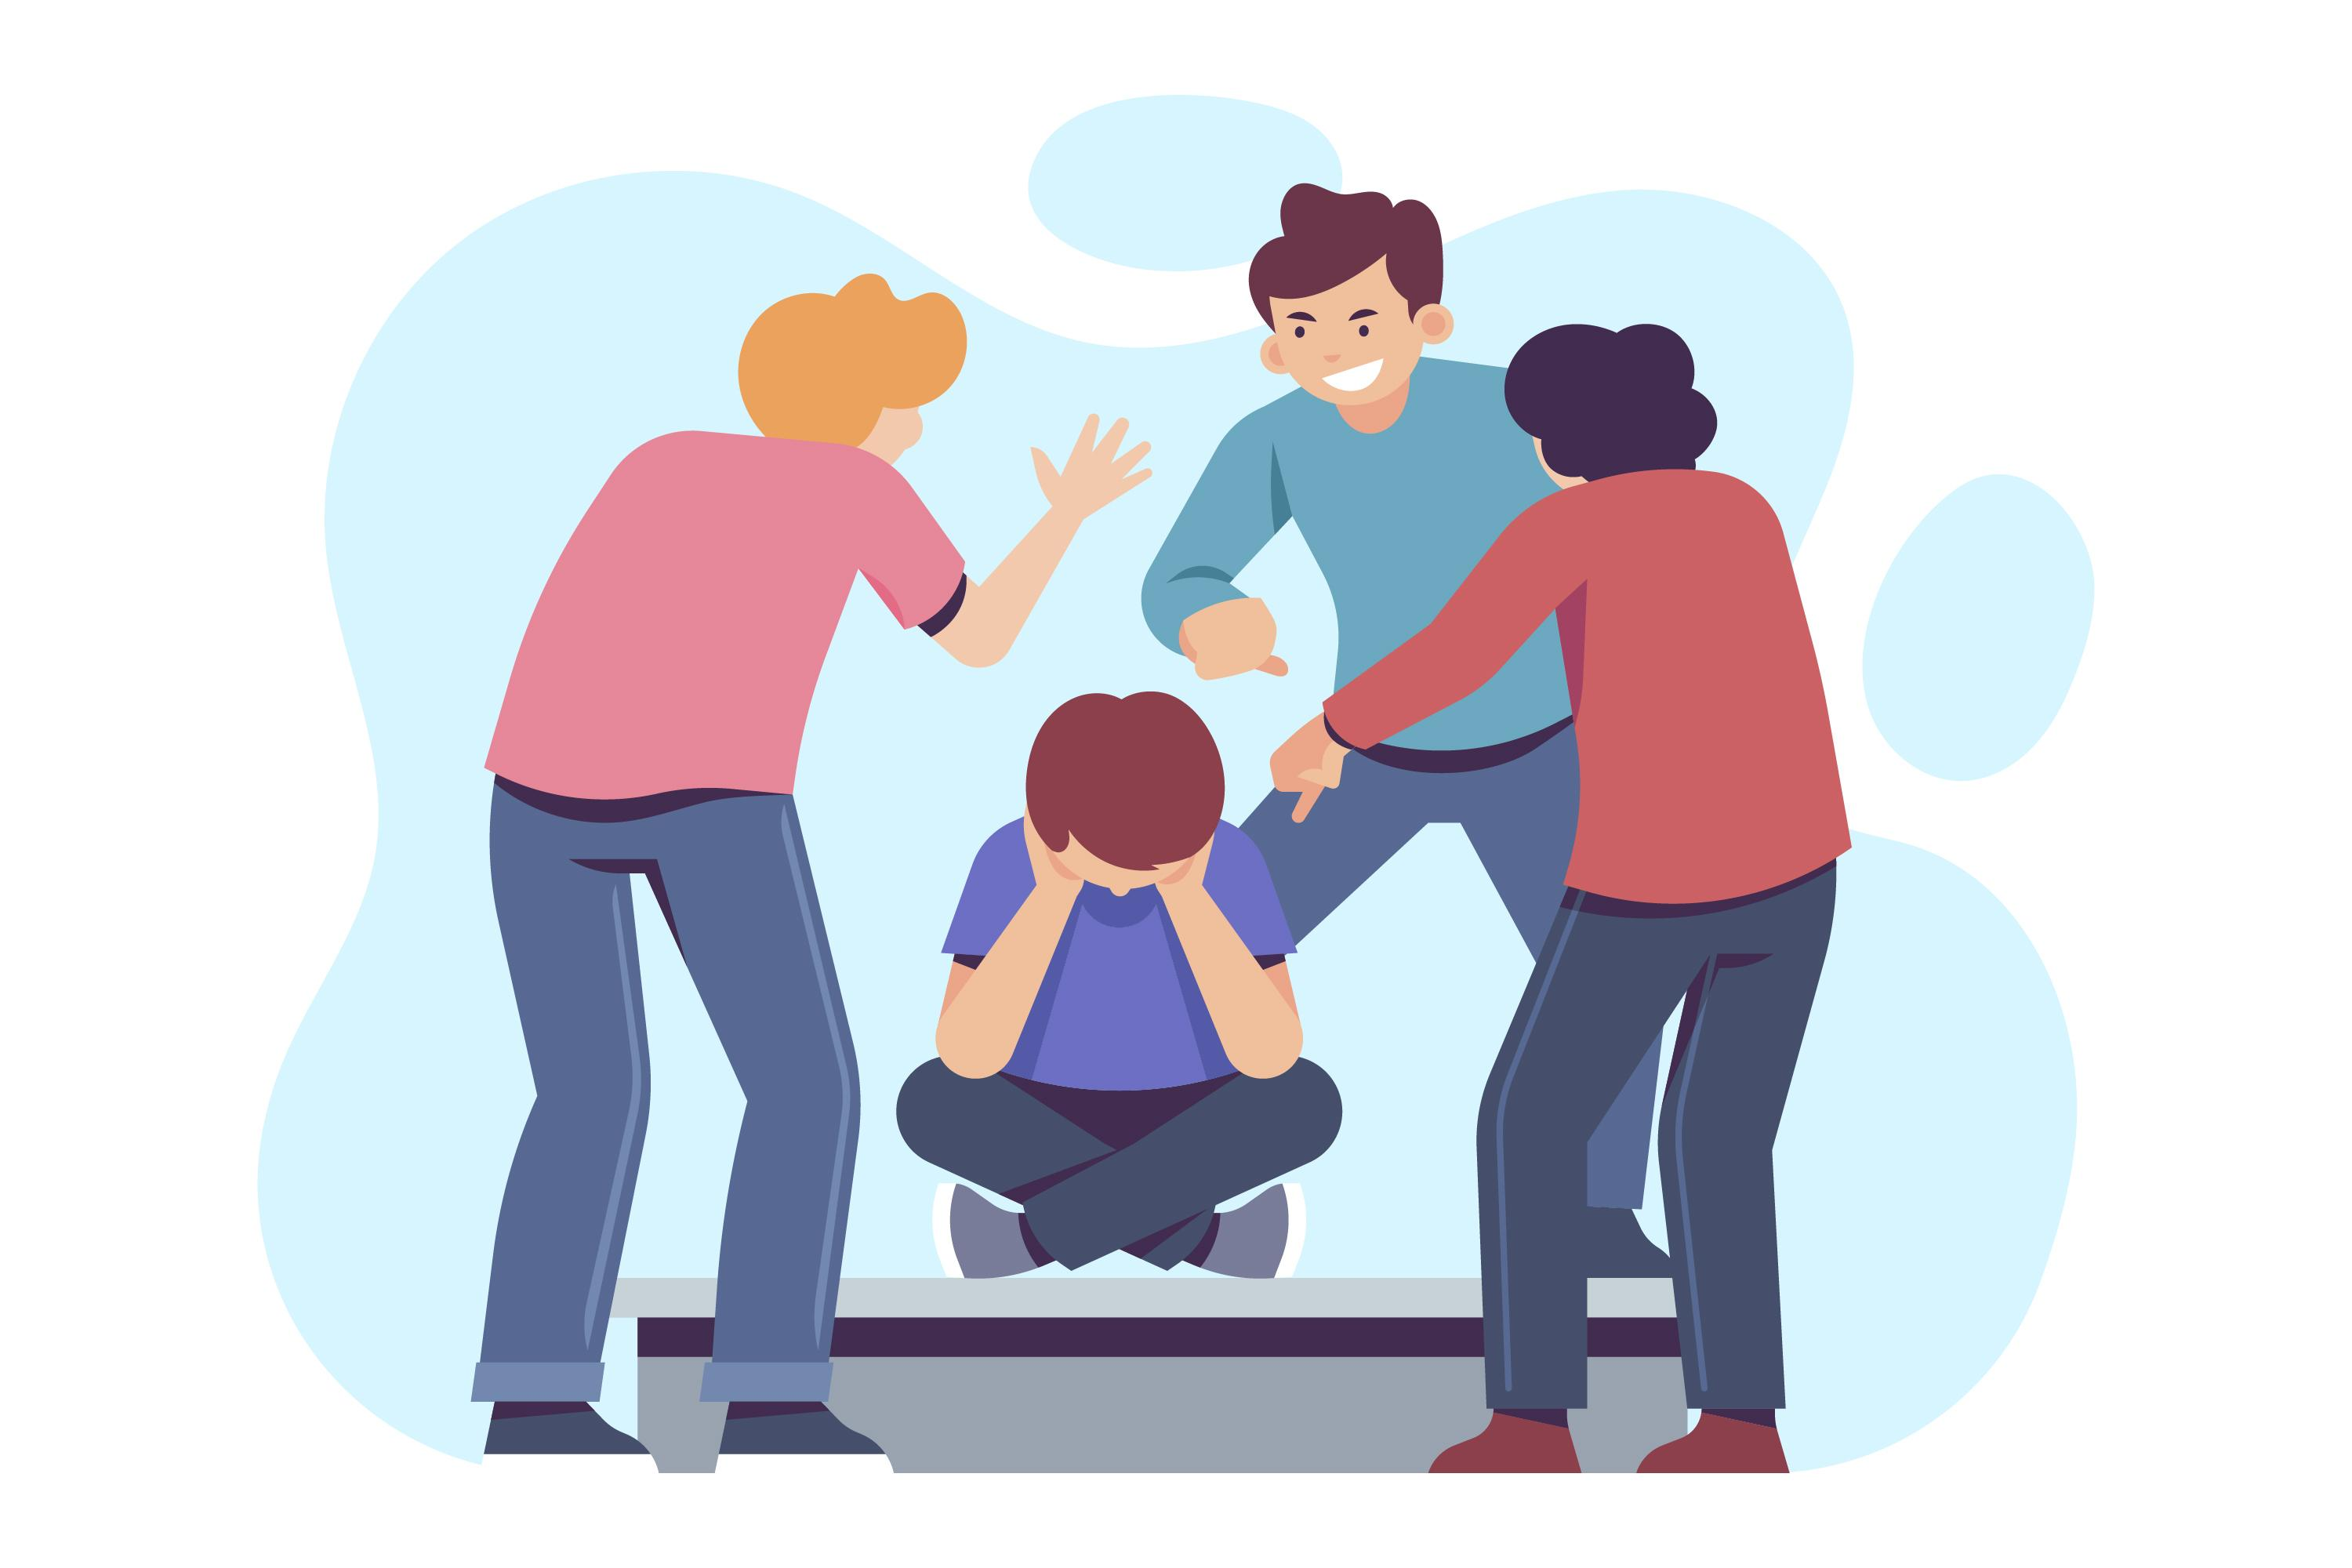
\includegraphics[width=0.7\textwidth]{./imgSAEB_6_POR/freepik/PORT_6_IMG-27.jpeg}
\end{figure}

\begin{quote}
\centering\textsc{Lembre-se: bullying não tem graça.}
\end{quote}

\noindent Em ``bullying não tem graça'', o advérbio ``não'' demonstra que o
\textbf{posicionamento do enunciador}, ou seja, de quem divulga a
campanha, é de:

\begin{escolha}
\item Negação em relação ao fato de o bullying ser um problema.
\item Certeza de que não tem diversão em se fazer bullying.
\item Condição, pois só se saberá se será engraçada a ação depois de ela
concretizada.
\item Possibilidade de que o bullying seja engraçado.
\end{escolha}

%\paragraph{BNCC: EF69LP04} 
% Identificar e analisar os efeitos de sentido que
% fortalecem a persuasão nos textos publicitários, relacionando as
% estratégias de persuasão e apelo ao consumo com os recursos
% linguístico-discursivos utilizados, como imagens, tempo verbal, jogos de
% palavras, figuras de linguagem etc., com vistas a fomentar práticas de
% consumo conscientes.

% Gabarito, treino?
% \begin{escolha}
% \item Incorreta. O advérbio de negação, aqui, não nega o posicionamento do
% enunciador da campanha, pelo contrário, ele o afirma.
% \item Correta. Embora seja um advérbio de negação, enquanto modalizador do
% discurso ele funciona como um reforço de certeza, afirmação, no
% enunciado de que Bullying não é legal.
% \item Incorreta. Não existe uma condição para que o enunciador considere o
% bullying legal ou não.
% \item Incorreta. Não é uma possibilidade o bullying ser ou não legal.
% \end{escolha}

\num{2} Leia o trecho a seguir.

\begin{quote}
\centering\textbf{Jogos eletrônicos podem desenvolver dependência e prejudicar
desenvolvimento infantil}\\
\medskip


\noindent Na China, o acesso a videogames por crianças e adolescentes menores de
idade é restrito. O país libera os jogos on-line para esse grupo somente
durante as sextas-feiras, fins de semana e feriados, com horário
predeterminado e o limite de jogo por no máximo três horas semanais. A
medida foi tomada com o objetivo de prevenir o vício e combater o que
tem sido chamado de ``ópio do espírito'' pela mídia chinesa.

Entretanto, na avaliação de Valdemar Setzer, professor titular sênior do
Departamento de Ciência da Computação do Instituto de Matemática e
Estatística da USP, a proibição não é a melhor estratégia. ``Em
princípio, eu sou contra proibições, pois elas vão contra a liberdade
das pessoas. A gente deveria conscientizá-las'', afirma. ``Mas,
infelizmente, os adultos não estão tendo consciência e conhecimento para
eles próprios adotarem as atitudes corretas'', acrescenta o professor,
ao comentar que os limites deveriam ser impostos por pais, mães e
responsáveis pelas crianças.

\fonte{Rodrigo Tammako e Patrick Fuentes. Jornal da USP. Jogos eletrônicos
podem desenvolver dependência e prejudicar desenvolvimento infantil.
Disponível em: https://jornal.usp.br/atualidades/jogos-eletronicos-podem-desenvolver-dependencia-e-prejudicar-desenvolvimento-infantil.
Acesso em: 21 mar. 2023. Adaptado.}
\end{quote}

\noindent O termo ``Em princípio'' é usado pelo especialista a fim de

\begin{escolha}
\item Elencar mais de um posicionamento sobre o uso de jogos eletrônicos
por crianças e adolescentes.
\item Preparar o leitor para uma informação contraditória que ele irá
apresentar.
\item Demonstrar ao leitor que irá começar a apresentar seu posicionamento
dali adiante.
\item Apresentar em primeiro lugar o que ele pensa sobre um outro assunto,
antes de voltar ao tema do texto.
\end{escolha}

%\paragraph{BNCC: EF69LP04} 
% Identificar e analisar os efeitos de sentido que
% fortalecem a persuasão nos textos publicitários, relacionando as
% estratégias de persuasão e apelo ao consumo com os recursos
% linguístico-discursivos utilizados, como imagens, tempo verbal, jogos de
% palavras, figuras de linguagem etc., com vistas a fomentar práticas de
% consumo conscientes.

% Gabarito, treino?
% \begin{escolha}
% \item Incorreta. O especialista coloca apenas um posicionamento: ele é a
% favor da proibição em alguns casos.
% \item Incorreta. O especialista não se contradiz. Ele é contraditório à
% proibição dos jogos.
% \item Correta. O objetivo do especialista é demarcar para o leitor que irá
% começar a apresentar seu posicionamento dali adiante.
% \item Incorreta. O especialista fala apenas sobre um assunto: ele é contra
% a proibição, e justifica seu posicionamento.
% \end{escolha}

\num{3} ``Em princípio, eu sou contra proibições, pois elas vão contra a
liberdade das pessoas. A gente deveria conscientizá-las'', afirma. Se o
verbo ``deveria'' fosse substituído por ``poderia'', o efeito de sentido
da frase seria de:

\begin{escolha}
\item Condição.
\item Obrigação.
\item Contradição.
\item Necessidade.
\end{escolha}

%\paragraph{BNCC: EF69LP04} 
% Identificar e analisar os efeitos de sentido que
% fortalecem a persuasão nos textos publicitários, relacionando as
% estratégias de persuasão e apelo ao consumo com os recursos
% linguístico-discursivos utilizados, como imagens, tempo verbal, jogos de
% palavras, figuras de linguagem etc., com vistas a fomentar práticas de
% consumo conscientes.

% Gabarito, treino?
% \begin{escolha}
% \item Correta. Ao trocar o verbo ``deveria'', que exprime uma
% obrigatoriedade, por ``poderia'', a frase toma o sentido de condição, ou
% seja, poderiam ou não ser conscientizadas a depender de alguma
% circunstância.
% \item Incorreta. O verbo ``poderia'' exprime possibilidade mediante
% condição. O verbo ``dever'' já está representando obrigatoriedade.
% \item Incorreta. O verbo ``poderia'' não geraria contradição, haveria
% apenas modificação de sentido.
% \item Incorreta. O verbo ``poderia'' não exprime necessidade ou obrigação,
% se inserido nesse contexto.
% \end{escolha}

\chapter{As figuras de linguagem}
\markboth{Módulo 9}{}

\section{Habilidades do SAEB}
\begin{itemize}
\item Analisar o uso de figuras de linguagem como
estratégia argumentativa.
\item Avaliar a eficácia das estratégias
argumentativas em textos de diferentes gêneros.
\end{itemize}

\subsection{Habilidades da BNCC} 
\begin{itemize}
\item EF69LP17
\item EF67LP38
\end{itemize}

\conteudo{Figuras de linguagem são recursos utilizados para expressar ideias e
emoções de forma mais intensa, criativa e poética. São usadas para
enriquecer o discurso, tornando-o mais expressivo e marcante.

Algumas das figuras de linguagem mais comuns são:

\paragraph{Metáfora} comparação implícita entre duas coisas que têm
características em comum;

\paragraph{Metonímia} uso de uma palavra ou expressão no lugar de outra, com a
qual se relaciona de alguma forma;

\paragraph{Hipérbole} exagero proposital para enfatizar uma ideia ou emoção;

\paragraph{Ironia} uso de palavras que aparentemente significam o oposto do que
se quer dizer, com o objetivo de criticar ou provocar um efeito de
humor;

\paragraph{Personificação} atribuição de características humanas a seres
inanimados ou animais;

\paragraph{Catacrese} quando uma palavra é usada de forma aproximada ou adaptada, por falta de um termo mais adequado, como "asa da xícara" ou "pé da cama";

\paragraph{Sinestesia} ocorre quando uma expressão mistura duas sensações
diferentes entre aquelas percebidas pelos órgãos sensoriais;

\paragraph{Gradação} sequência de palavras que intensifica uma ideia;

\paragraph{Eufemismo} expressões usadas para atenuar uma ideia tida como
agressiva ou desagradável;

\paragraph{Onomatopeia} representação gráfica dos sons;

\paragraph{Aliteração} repetição de sosns consonantais idênticos ou semelhantes para
sugerir acusticamente algum elemento, ato, fenômeno;

\paragraph{Pleonasmo} construção em que se expressam as ideias de forma redundante, para enfatizá-las.}

\conteudo{
As figuras de linguagem são usadas para:

\paragraph{Tornar a mensagem mais expressiva:} podem tornar a mensagem mais
marcante, expressiva e poética, tornando-a mais impactante para quem
ouve ou lê.

\paragraph{Enfatizar ideias} algumas figuras de linguagem, como a hipérbole,
são usadas para enfatizar ideias ou emoções, aumentando o impacto da
mensagem.

\paragraph{Facilitar a compreensão} a metáfora e a comparação podem ser usadas
para facilitar a compreensão de ideias abstratas ou complexas,
tornando-as mais concretas e acessíveis.

\paragraph{Criar efeitos de humor} a ironia e o sarcasmo podem ser usados para
criar efeitos de humor, tornando a mensagem mais leve e descontraída.

\paragraph{Estimular a imaginação} a personificação e a metáfora estimulam a
imaginação do leitor ou ouvinte, permitindo que ele visualize a mensagem
de forma mais vívida e intensa.

\paragraph{Criar identificação:} a metonímia, por exemplo, é usada para criar
identificação entre a mensagem e o contexto em que ela está sendo
utilizada, tornando-a mais pessoal e próxima do leitor ou ouvinte.}

\section{Atividades}

\noindent Observe a campanha de conscientização a seguir, composta de imagem e de
texto, para responder às questões de 1 a 4.

\begin{figure}[H]
%PORT_6_IMG-28 — POR.tex:3266
\centering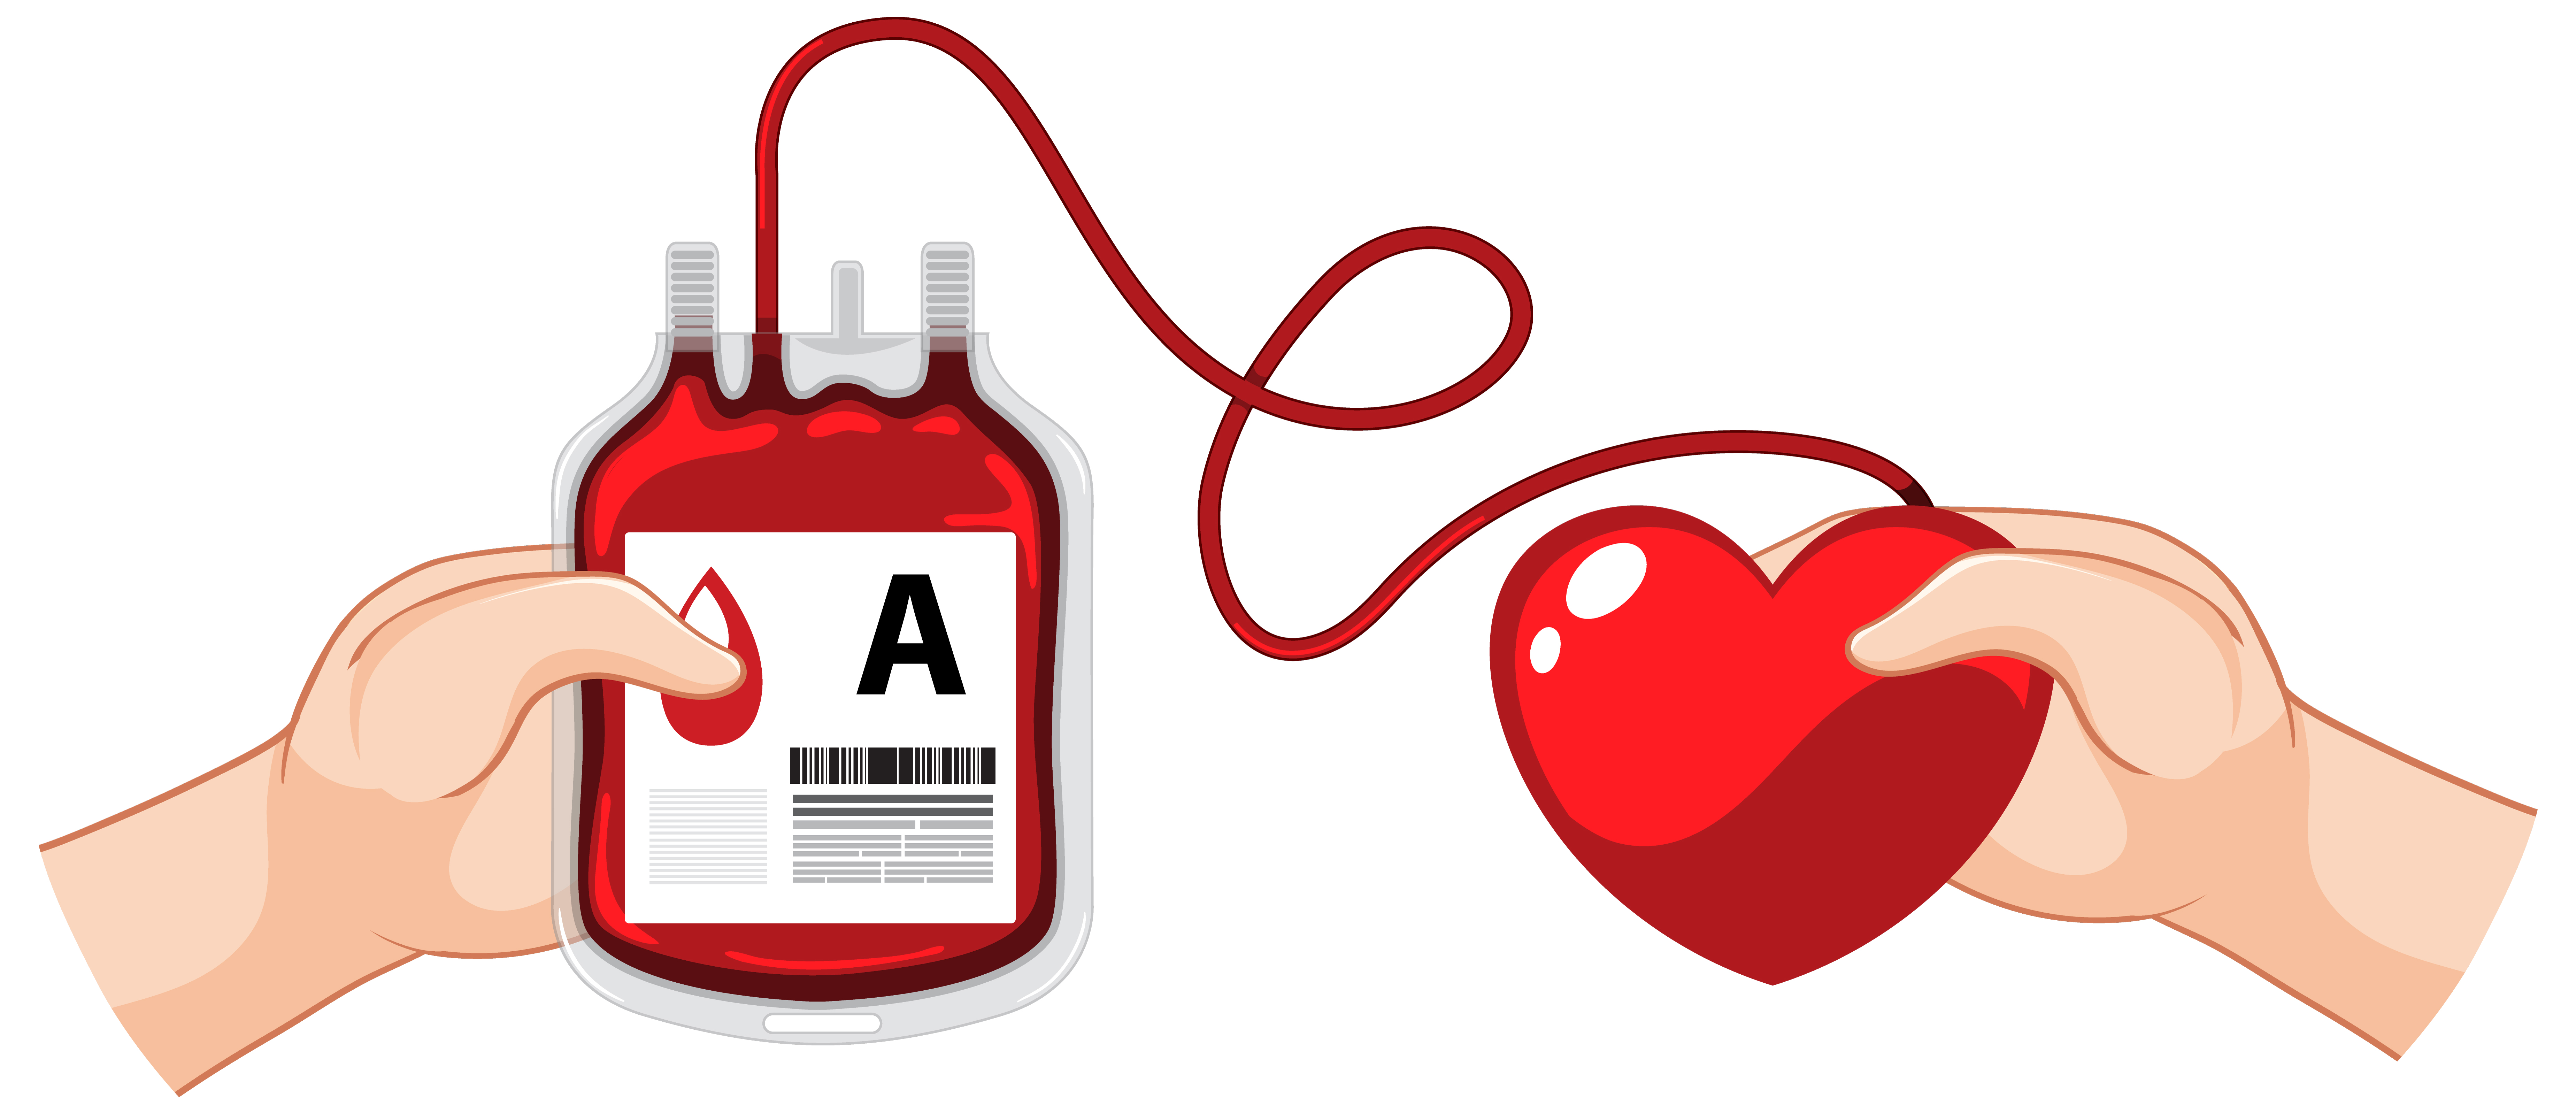
\includegraphics[width=0.7\textwidth]{./imgSAEB_6_POR/freepik/PORT_6_IMG-28.jpeg}
\end{figure}

\num{1} Qual é o objetivo da campanha?

\reduline{O objetivo é incentivar as pessoas a doarem sangue.\hfill}\linhas{1}

\num{2} Que recursos a campanha utiliza para argumentar a favor dessa
ideia?

\reduline{A campanha compara o sangue doado a um presente.\hfill}\linhas{1}

\num{3} Qual a importância da imagem utilizada na campanha?

\reduline{A imagem associa o doador de sangue, por meio da imagem da bolsa, ao coração do receptor, por meio do ícone do órgão. O coração, nesse caso, representa a vida.\hfill}\linhas{1}

\num{4} Que figura de linguagem predomina na propaganda?

\reduline{A metáfora é a figura predominante na campanha.\hfill}\linhas{1}

\pagebreak

\noindent Leia o diálogo a seguir e responda às questões de 5 a 8.


\begin{figure}[H]
%PORT_6_IMG-29 — POR.tex:3297
\centering\includegraphics[width=0.7\textwidth]{./imgSAEB_6_POR/freepik/PORT_6_IMG-29.jpeg}
\end{figure}

\begin{quote}
--- Aninha, você acha que a gente ganha o interclasses neste semestre?

--- Lógico, Gael. Eu até já sinto o cheiro do brilho do troféu!

--- Que cheiro ele tem?

--- Agora tá parecendo cheiro de lanche da cantina. Que horas são?
\end{quote}

\num{5} Em ``Aninha, você acha que a gente ganha o interclasses neste
semestre?'', qual é a figura de linguagem presente? O que a fala da
personagem significa?

\reduline{A figura de linguagem presente é a metonímia, ou seja, quando
há substituição da parte pelo todo. O menino substitui a palavra
``campeonato'' pelo nome desse campeonato em questão, ``interclasse''.\hfill}\linhas{1}

\num{6} Em ``já sinto o cheiro do brilho do troféu'', qual é a figura de
linguagem presente? O que a fala da personagem significa?

\reduline{A figura de linguagem presente é a sinestesia. A personagem
quis dizer que ela pressentia que iriam vencer o campeonato.\hfill}\linhas{1}

\num{7} Em qual momento da história é possível identificar o efeito de
humor da tirinha? Como esse humor se constrói?

\reduline{Quando o cheiro "figurado" da vitória é substituído pelo cheiro "real" do lanche da cantina, acontece uma quebra de expectativa que gera humor.\hfill}\linhas{1}

\num{8} Como se pode interpretar a relação entre a pergunta ``Que horas
são?'' e o restante do diálogo?

\reduline{O fato de Aninha sentir cheiro do lanche provavelmente mostra que ela está com fome ou com vontade de comer - assim, a pergunta sobre o horário pode ser para ela saber se eles estão próximos do momento do intervalo, já que é nesse horário que geralmente os alunos comem lanche na cantina.\hfill}\linhas{1}

\num{9} Assinale a alternativa que contém uma catacrese.

\begin{escolha}
\item Meu avô é sábio, grande, fantástico!
\item O jogo me causou muita dor na batata da perna.
\item Mariana tinha uma voz doce, delicada e macia.
\item O bebê comeu o prato todo de papinha no almoço!
\end{escolha}

% Gabarito, treino?
% \coment{
% \begin{escolha}
% \item Incorreta. A figura de linguagem presente na frase é a gradação.
% \item Correta. Costuma-se utilizar o termo "batata da perna" para
% referir-se à panturrilha por comparação.
% \item Incorreta. A figura de linguagem presente na frase é a sinestesia.
% \item Incorreta. A figura de linguagem presente na frase é a metonímia.
% \end{escolha}}

\num{10} Leia o texto a seguir.

\begin{quote}
Eu acho que a pior invenção da vida é mingau de fubá. Não compreendo
para que ele serve. Se a gente está com fome, toma mingau e a fome
aperta mais. Se não está com fome, bebe mingau e a fome abre. Há tanta
coisa boa para se fazer com fubá: cuscuz, broas, sonhos, bolos, e
ninguém quer sair do mingau de fubá.

\fonte{Helena Morley. \emph{Minha vida de menina}. São Paulo: Companhia de
Bolso, 2016.}
\end{quote}

\noindent Explique como a figura da personificação aparece no trecho.

\reduline{No trecho, aparece personificação quando se diz que "a fome aperta" e "a forme abre".\hfill}\linhas{2}

\section{Treino}

\num{1} Leia o texto a seguir.

\begin{quote}
{[}\ldots{]} de tanto pensar no LOBO, de tanto sonhar com LOBO, de tanto
esperar o LOBO, um dia topou com ele que era assim: carão de LOBO, olhão
de LOBO, jeitão de LOBO {[}\ldots{]}.

\fonte{Chico Buarque. Chapeuzinho Amarelo. Ilustrações de Ziraldo. Belo
Horizonte: Autêntica, 2017.}
\end{quote}

% \begin{figure}[H]
% %PORT_6_IMG-30 — POR.tex:3373
% \centering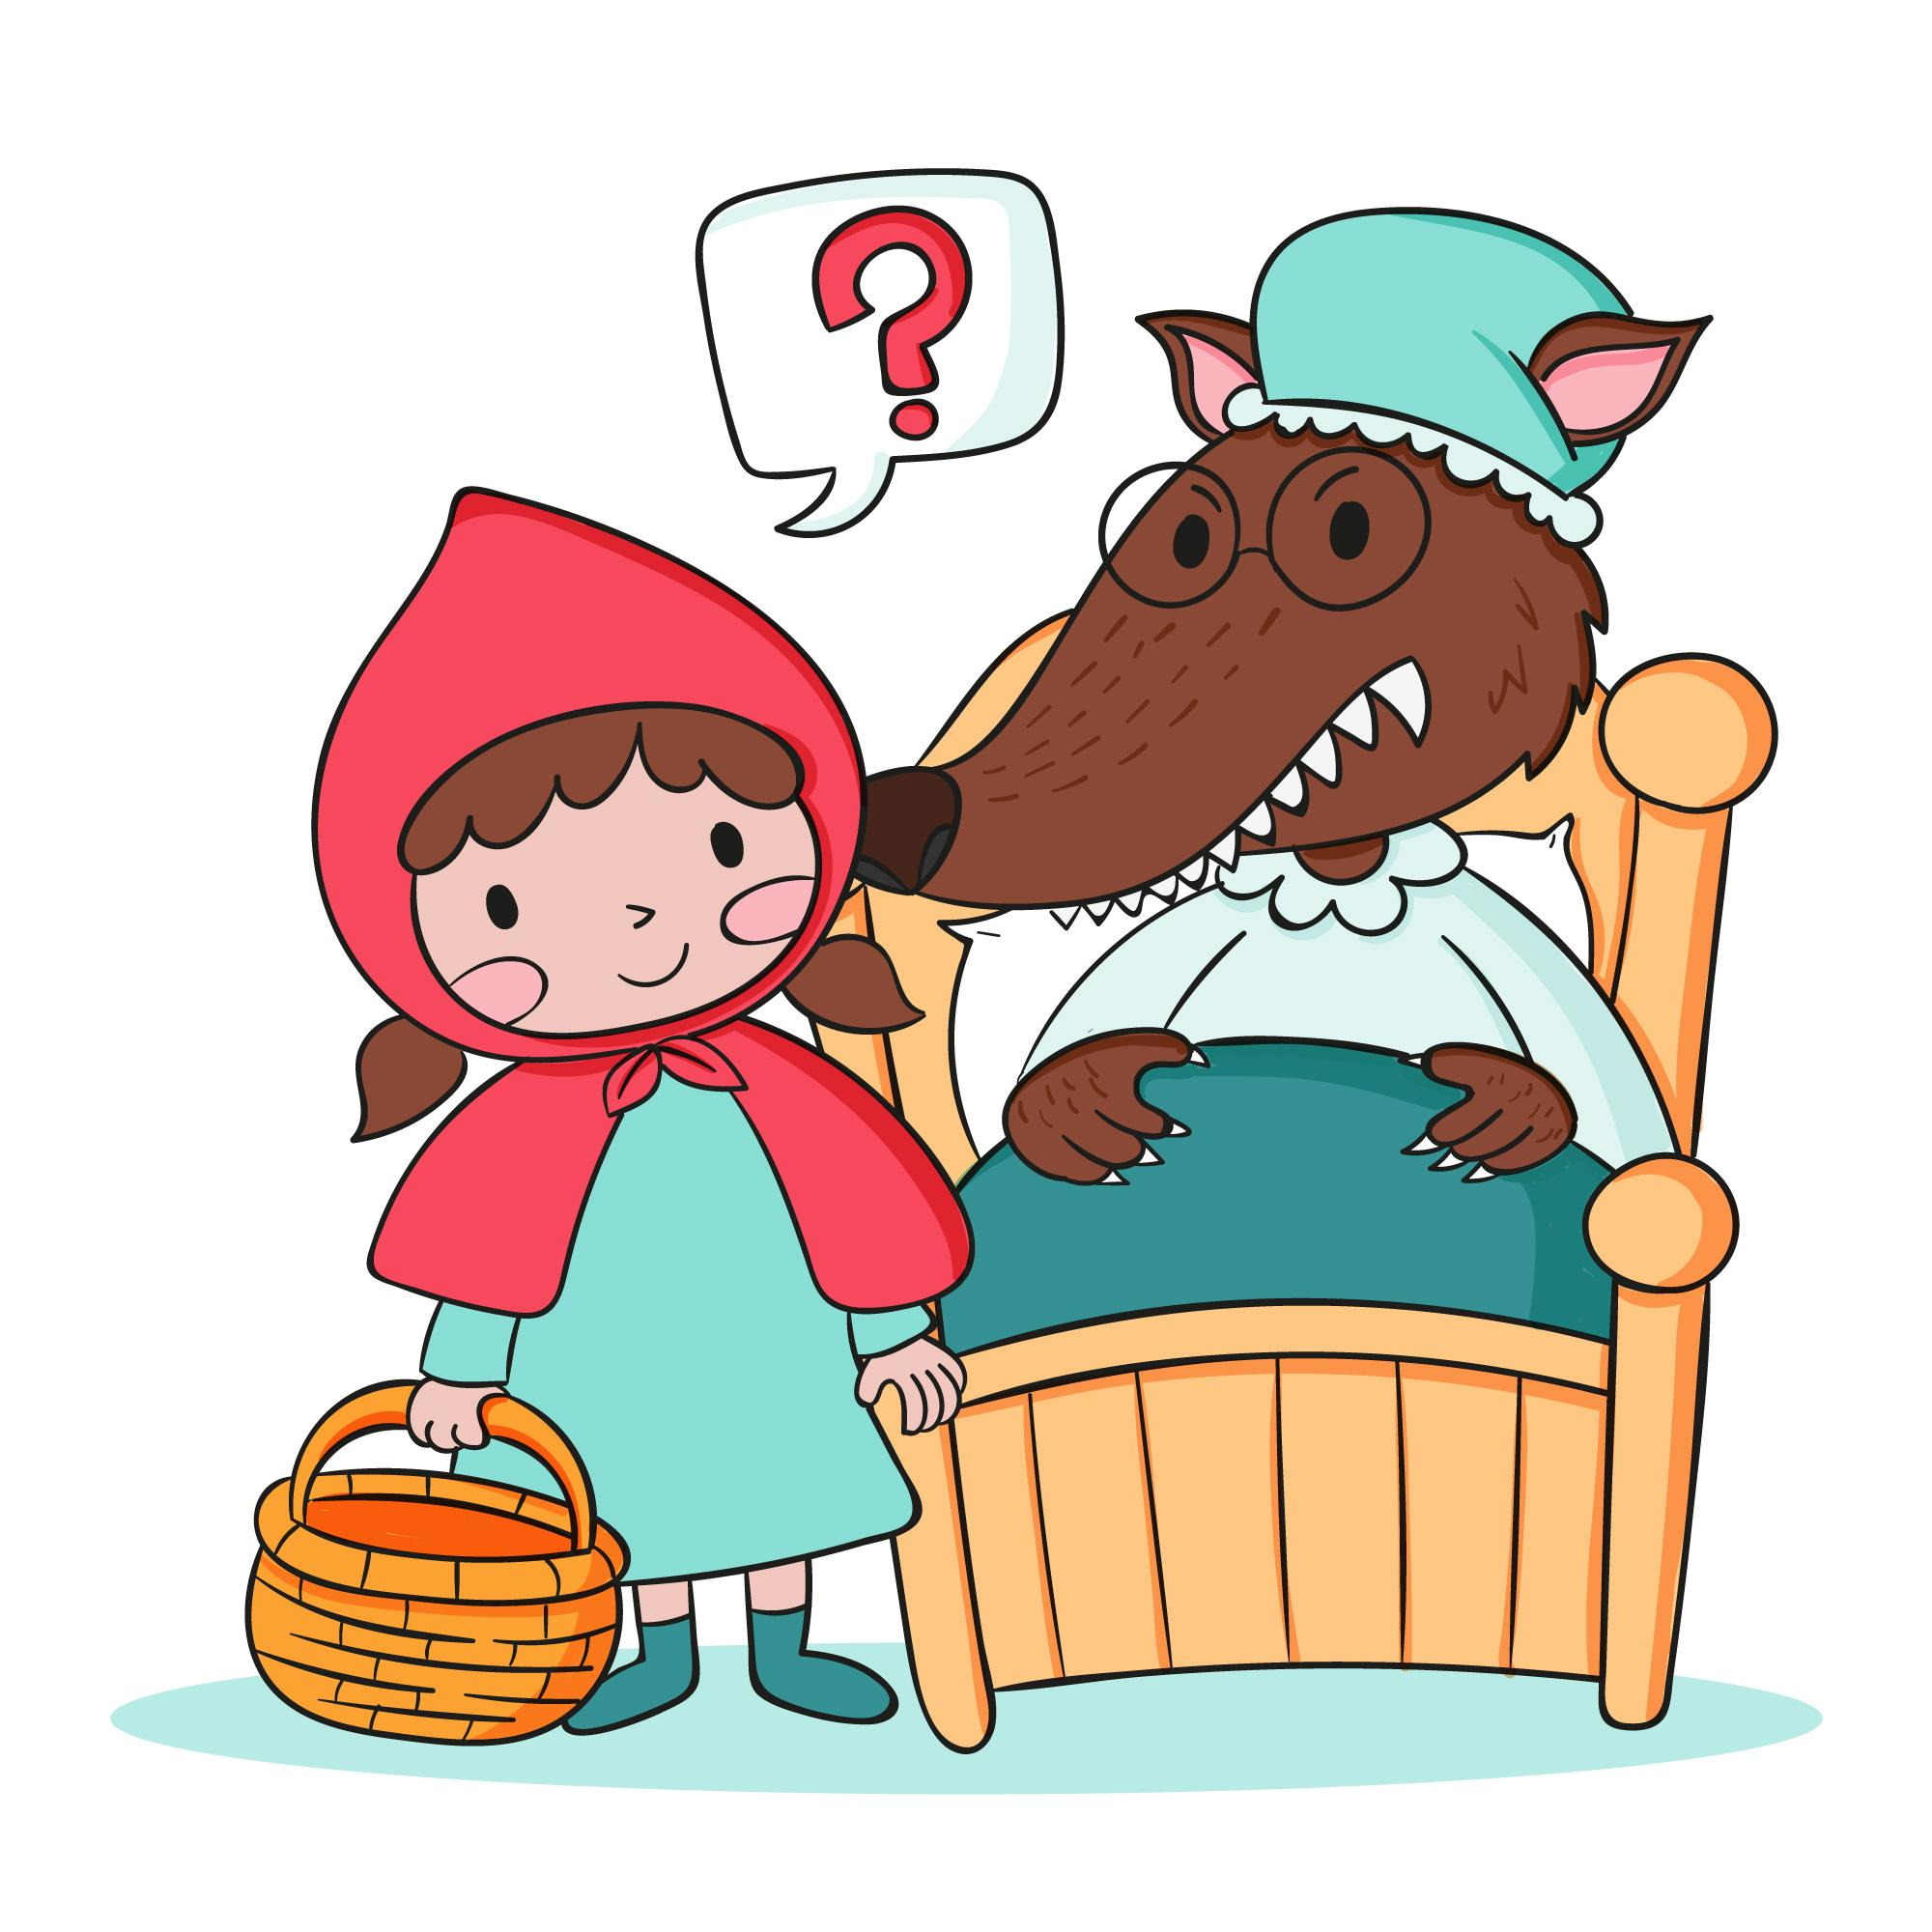
\includegraphics[width=0.7\textwidth]{./imgSAEB_6_POR/freepik/PORT_6_IMG-30.jpeg}
% \end{figure}

A figura de linguagem representada no trecho pela repetição do fonema
/bo/ é:

\begin{escolha}
\item Onomatopeia.
\item Aliteração.
\item Pleonasmo.
\item Metáfora.
\end{escolha}

%\paragraph{BNCC: EF67LP38} 
% Analisar os efeitos de sentido do uso de figuras de
% linguagem, como comparação, metáfora, metonímia, personificação,
% hipérbole, dentre outras.

% Gabarito, treino?
% \begin{escolha}
% \item Incorreta. Onomatopeia é a representação gráfica dos sons.
% \item Correta. Aliteração é a repetição de sons consonantais idênticos ou
% semelhantes para sugerir acusticamente algum elemento, ato, fenômeno.
% \item Incorreta. Pleonasmo é uma figura de linguagem que expressa a
% redundância.
% \item Incorreta. Metáfora é uma comparação implícita entre duas coisas que
% têm características em comum.
% \end{escolha}

\num{2} Observe a imagem a seguir, que apresenta apenas texto não verbal
para promover a necessidade de cuidarmos do meio ambiente.

\begin{figure}[H]
%PORT_6_IMG-31 — POR.tex:3411
\centering\includegraphics[width=0.7\textwidth]{./imgSAEB_6_POR/freepik/PORT_6_IMG-31.jpeg}
\end{figure}

\noindent O argumento utilizado na campanha que incentiva o combate ao
desmatamento é:

\pagebreak
\begin{escolha}
\item Uma metáfora.
\item Um eufemismo.
\item Uma hipérbole.
\item Uma personificação.
\end{escolha}

%\paragraph{BNCC: EF67LP38} 
% Analisar os efeitos de sentido do uso de figuras de
% linguagem, como comparação, metáfora, metonímia, personificação,
% hipérbole, dentre outras.

% Gabarito, treino?
% \begin{escolha}
% \item Correta. A campanha argumenta comparando a proteção ao Meio Ambiente
% a uma ideia, representada visualmente pela lâmpada.
% \item Incorreta. O eufemismo utiliza-se de expressões para atenuar uma
% ideia tida como agressiva ou desagradável.
% \item Incorreta. A hipérbole é o exagero proposital para enfatizar uma
% ideia ou emoção.
% \item Incorreta. A personificação consiste em atribuir características
% humanas a seres e objetos inanimados.
% \end{escolha}

\num{3} Leia um trecho de um artigo de opinião, a seguir.

\begin{figure}[h!]
%PORT_6_IMG-32 — POR.tex:3442
\centering\includegraphics[width=0.7\textwidth]{./imgSAEB_6_POR/freepik/PORT_6_IMG-32.jpeg}
\end{figure}

\begin{quote}
Mas o pai da aviação continua sendo Santos Dumont, não Boeing, Airbus,
Lockheed — que cuidaram, investiram e fizeram \textbf{aquela
saltitante criaturinha de bambu e seda} se transformar nesses galalaus
de alumínio — com péssimo serviço de bordo, diga-se de passagem.

\fonte{Eduardo Affonso. IG Opinião. Disponível em: 
\url{https://lulacerda.ig.com.br/opiniao-por-eduardo-affonso-pai-e-quem-cuida}.
Acesso em: 26 mar. 2023.}
\end{quote}

\noindent O efeito de humor apresentado no trecho em destaque, ``aquela saltitante
criaturinha de bambu e seda'', é dado por meio de:

\begin{escolha}
\item Metáfora.
\item Personificação.
\item Catacrese.
\item Metonímia.
\end{escolha}

%\paragraph{BNCC: EF67LP38} 
% Analisar os efeitos de sentido do uso de figuras de
% linguagem, como comparação, metáfora, metonímia, personificação,
% hipérbole, dentre outras.

% Gabarito, treino?
% \begin{escolha}
% \item Correta. Metáfora é uma comparação sem uso de conector, como acontece
% na passagem.
% \item Incorreta. A personificação consiste em atribuir características
% humanas a seres e objetos inanimados.
% \item Incorreta. A catacrese ocorre quando uma palavra é usada de forma
% aproximada, quando não se tem um termo mais específico.
% \item Incorreta. A criatura a que o texto se refere é o 14Bis, avião
% construído por Santos Dummont. Não ocorre metonímia.
% \end{escolha}


\chapter{Os pronomes em nosso dia a dia}
\markboth{Módulo 10}{}

\section{Habilidades do SAEB }
\begin{itemize}
\item Analisar os mecanismos que contribuem para a
progressão textual. 
\item Analisar os processos de referenciação lexical e
pronominal.
\end{itemize}

\subsection{Habilidade da BNCC}
\begin{itemize}
\item EF06LP12
\end{itemize}

\conteudo{
Na língua portuguesa, quando vamos nos referir a um substantivo,
empregamos algumas classes de palavras capazes de dar a ele limites de
significação. É o caso de artigos, adjetivos, numerais e pronomes.

Os pronomes são os responsáveis por relacionar o substantivo a uma das
três pessoas do discurso (quem fala, com quem se fala e de quem se
fala), podendo, ainda, indicar a posse de um objeto ou sua localização.
Quando substituem o nome, denominam-se pronomes substantivos;
quando o acompanham, pronomes adjetivos.

Os pronomes classificam-se em: pessoais, possessivos, demonstrativos,
interrogativos, indefinidos e relativos.

Ainda no campo semântico da língua, ou seja, aquele em que se estudam as classes de
palavras, vamos ressaltar neste módulo o estudo dos **sinônimos** (em
que palavras diferentes apresentem semelhante ou igual campo de
significação), \textbf{antônimos} (palavras referem-se a termos que apresentam sentidos
opostos entre si) e \textbf{homônimos} (palavras que coincidem na fala, na escrita ou em ambas).}

\section{Atividades}

\noindent Observe a imagem a seguir, leia o texto que a acompanha e responda às
questões de 1 a 4.

\pagebreak
\begin{figure}[H]
%PORT_6_IMG-33 — POR.tex:3514
\centering\includegraphics[width=0.7\textwidth]{./imgSAEB_6_POR/freepik/PORT_6_IMG-33.jpeg}
\end{figure}

\begin{verse}
\textbf{Todo grupinho da escola tem}\\
\medskip
O que faz cara de dó quando toma bronca\\
o que só ri\\
o que sempre faz piada\\
o que é bonzinho de verdade\\
o desligado\\
o que só tira nota alta\\
\end{verse}

\num{1} O texto está escrito em formato de meme. Reescreva o texto, na
forma de discurso direto, inserindo as pontuações necessárias.

\reduline{Todo grupinho da escola tem: o que faz cara de dó quando toma
bronca, o que só ri, o que sempre faz piada, o que é bonzinho de
verdade, o desligado e o que só tira nota alta.\hfill}\linhas{1}

\num{2} Na frase ``\textbf{todo} grupinho da escola tem'', qual é o
efeito de sentido provocado pelo pronome em destaque?

\reduline{"Todo" é um pronome indefinido, que traz ao texto a ideia de
generalização, porém sem nomear um grupo específico: qualquer grupo tem um aluno com aquelas características.\hfill}\linhas{1}

\num{3} Substitua os termos destacados a seguir por um sinônimo e um
antônimo, considerando o contexto.

\begin{escolha}
\item O que faz cara de \textbf{dó}
\begin{itemize}
\item Sinônimo: \reduline{Piedade.\hfill}
\item Antônimo: \reduline{Desprezo.\hfill}
\end{itemize}

\item O que só \textbf{ri}
\begin{itemize}
\item Sinônimo: \reduline{Gargalha; .\hfill}
\item Antônimo: \reduline{Chora.\hfill}
\end{itemize}

\item O que é \textbf{bonzinho}
\begin{itemize}
\item Sinônimo: \reduline{Cortês, gentil, solidário.\hfill}
\item Antônimo: \reduline{Malvado.\hfill}
\end{itemize}

\item O que só tira nota \textbf{alta}
\begin{itemize}
\item Sinônimo: \reduline{Boa.\hfill}
\item Antônimo: \reduline{Baixa.\hfill}
\end{itemize}
\end{escolha}

\num{4} Um dos cachorrinhos representa um tipo de aluno considerado
``desligado''. Escreva uma frase que contenha um efeito de sentido
\textbf{homônimo}, uma com efeito de sentido \textbf{antônimo} e outra
com efeito de sentido \textbf{sinônimo} ao contexto em que foi empregado
esse termo.

\begin{itemize}
\item Homônimo: \reduline{O ventilador da sala estava desligado, por isso estava calor.\hfill}
\item Antônimo: \reduline{João é muito atento à aula, sempre presta atenção à professora.\hfill}
\item Sinônimo: \reduline{João é desatento, quase não presta atenção na professora.\hfill}
\end{itemize}

\num{5} Preencha corretamente as lacunas com os pronomes ``eu'' ou
``mim''.

\begin{escolha}
\item Comprei muitas frutas para \reduline{Eu.\hfill} fazer uma sobremesa.
\item Pode emprestar para \reduline{Mim.\hfill} aquela borracha?
\item Este bolo é para \reduline{Eu.\hfill} comer?
\item Nada pode fazer para \reduline{Eu.\hfill} ficar, infelizmente.
\item Entre \reduline{Mim.\hfill} e você há um abismo de ressentimentos.
\item Pode fazer aquela comida gostosa para \reduline{Mim.\hfill}?
\end{escolha}

\noindent Leia um excerto da crônica ``O lápis'', de Mário Prata, e responda aos
exercícios de 6 a 9.

\begin{quote}
É aqui que eu queria chegar. Não adianta o governo testar alunos e
professores e universidades. Vai dar sempre zebra. O buraco é bem mais
embaixo, senhor Ministro da Educação. Vamos voltar ao lápis e ao dois
mais dois. Vamos começar pela base. Vamos escrever a lápis. Mesmo
porque, se não der certo, a gente apaga e começa de novo.

\fonte{Mario Prata. O lápis. Disponível em: https://marioprata.net/cronicas/o-lapis. Acesso em: 15 mar. 2023. Adaptado.}
\end{quote}

\num{6} Substitua os termos em destaque na frase pelos pronomes pessoais
adequados.

\noindent Não adianta \textbf{o governo} testar \textbf{alunos e professores e
universidades}.

\reduline{Não adianta ele os testar.\hfill}\linhas{1}

\num{7} Em ``É aqui que eu queria chegar'' o enunciador se refere, de
fato, a um lugar geográfico? Explique.

\reduline{Não se trata de uma referência a um lugar físico, mas sim, da referência a um ponto da argumentação a que o enunciador queria chegar em seu texto.\hfill}\linhas{1}

\num{8} O que significa a palavra ``zebra'' no contexto em que aparece?
Que sinônimo poderia substituir essa palavra no texto?

\reduline{Nesse contexto, a palavra significa "problema" ou "resultado ruim". Um bom sinônimo seria a própria palavra "problema".\hfill}\linhas{1}

\num{9} Reescreva o trecho a seguir, a fim de eliminar as repetições.

Vamos voltar ao lápis e ao dois mais dois. Vamos começar pela base.
Vamos escrever a lápis. Mesmo porque, se não der certo, a gente apaga e
começa de novo."

\reduline{Vamos voltar ao lápis, ao dois mais dois, começar pela base e
escrever a lápis, porque, se não der certo, nós apagamos e começamos de
novo.\hfill}\linhas{1}

\num{10} Observe a campanha, composta de imagem e slogan.

\begin{figure}[H]
%PORT_6_IMG-34 — POR.tex:3672
\centering\includegraphics[width=0.7\textwidth]{./imgSAEB_6_POR/freepik/PORT_6_IMG-34.jpeg}
\end{figure}

\begin{quote}
\centering{Quanta comida se desperdiça no mundo? E quanta gente passa fome?}
\end{quote}

\noindent Reescreva o slogan, composto por duas frases interrogativas,
transformando-as em frases afirmativas e fazendo os ajustes necessários.

\reduline{Desperdiça-se muita comida no mundo. Muita gente passa fome.\hfill}\linhas{1}

\section{Treino}

\num{1} Leia o texto a seguir.

\begin{quote}
\textbf{O Brasil precisa do SUS: lançada campanha nacional de defesa do
Sistema Único de Saúde}\\
\medskip

\noindent A coordenadora do Campus Virtual Fiocruz, Ana Furniel {[}\ldots{]}
aponta que o Sistema Único de Saúde é imprescindível para o país. Seu
papel na pandemia ressaltou ainda mais a sua importância. {[}\ldots{]}

\fonte{Isabela Schincariol. Fiocruz. \emph{O Brasil precisa do SUS: lançada
campanha nacional de defesa do Sistema Único de Saúde}. Disponível em: https://campusvirtual.fiocruz.br/portal/?q=noticia/59976. Acesso em: 12 mar. 2023.}
\end{quote}

\noindent Em ``Seu papel na pandemia ressaltou ainda mais a sua importância.'', os
pronomes possessivos \emph{seu} e \emph{sua} referem-se:

\begin{escolha}
\item Ao SUS e à coordenadora do Campus Virtual Fiocruz.
\item Ao SUS, ambos.
\item À coordenadora do Campus Virtual Fiocruz, apenas.
\item À campanha \#OBrasilPrecisadoSUS.
\end{escolha}

%\paragraph{BNCC: EF06LP12} 
% Utilizar, ao produzir texto, recursos de coesão
% referencial (nome e pronomes), recursos semânticos de sinonímia,
% antonímia e homonímia e mecanismos de representação de diferentes vozes
% (discurso direto e indireto).

% Gabarito, treino?
% \begin{escolha}
% \item Incorreta. Não há referência à profissional, apenas ao sistema.
% \item Correta. Os pronomes referem-se ambos ao SUS.
% \item Incorreta. Os pronomes fazem referência à importância do SUS.
% \item Incorreta. Os pronomes fazem referência ao último substantivo do qual
% se fala, no caso, o SUS; e concordam, inclusive, com ele.
% \end{escolha}

\num{2} Leia o texto a seguir.

\begin{quote}
\noindent Ruth Rocha recebeu a equipe da TV Brasil em sua residência, em São
Paulo, para um papo sobre sua trajetória no universo literário e a
importância da leitura para as novas gerações.

Na entrevista, a escritora diz que é preciso conversar com as crianças
pois elas entendem mais do que se imagina. A autora conta que entende e
gosta de falar para as crianças de ontem e de hoje.

Ruth Rocha também destaca a importância do professor na formação do
público leitor. "O professor deve ler o livro antes e, se gostar, ler
para os alunos. Todos têm que gostar para dar certo", sugere a veterana
que adora ler e continua lendo de tudo.

Reverenciada pela crítica e pelo público, a autora foi reconhecida com
diversos prêmios como o Jabuti.

\fonte{Disponível em: https://tvbrasil.ebc.com.br/entrevista-com-ruth-rocha-e-destaques-no-dia-das-criancas. Acesso em: 23 mar. 2023. Adaptado.}
\end{quote}

\noindent Na fala de Ruth Rocha, o pronome ``todos'' refere-se a(aos):

\begin{escolha}
\item Aos alunos.
\item Aos livros.
\item Aos professores.
\item A alunos e professores.
\end{escolha}

%\paragraph{BNCC: EF06LP12} 
% Utilizar, ao produzir texto, recursos de coesão
% referencial (nome e pronomes), recursos semânticos de sinonímia,
% antonímia e homonímia e mecanismos de representação de diferentes vozes
% (discurso direto e indireto).

% Gabarito, treino?
% \begin{escolha}
% \item Incorreta. O pronome refere-se a alunos e professores.
% \item Incorreta. A fala de Ruth Rocha não faz qualquer menção a livros no
% plural. O pronome acompanha o substantivo em número.
% \item Incorreta. O pronome refere-se a alunos e professores, todos têm que
% gostar do livro.
% \item Correta. O pronome faz referência a alunos e professores, o que é
% reforçado pelo fato de o verbo estar na 3ª pessoa do plural.
% \end{escolha}

\num{3} Leia o texto a seguir.

\begin{quote}
\centering\noindent \textbf{Sabores sem fronteiras}\\

\noindent \emph{Livro com receitas de refugiados é um convite para conhecer
trajetórias de vida e sabores}\\
\medskip

\noindent Ricardo nasceu em Caracas, o segundo de quatro irmãos. ``Meu gosto pela
cozinha vem desde muito jovem. Lembro com emoção de minha avó ensinando
as receitas de família para os filhos e filhas, e depois netos e netas.
\textbf{Esta} receita traz boas lembranças dessa época''. Ricardo veio
para o Brasil em 2015, para se casar com uma brasileira que conheceu
quando era guia turístico na Venezuela. Ele sempre prepara o
\emph{sancocho} em sua casa no bairro do Butantã, em São Paulo.

\fonte{Patrícia Mariuzzo. Sabores sem fronteiras. Disponível em: https://www.unicamp.br/unicamp/ju/noticias/2022/02/07/sabores-sem-fronteiras. Acesso em: 7 mar. 2023. Adaptado.}
\end{quote}

\noindent A escolha do pronome ``esta'', ao se referir ao \emph{sancocho},
está correta pois o enunciador

\begin{escolha}
\item está geograficamente próximo ao prato.
\item patenteou a receita.
\item menciona a receita depois de aparecer o pronome.
\item quer que o leitor se sinta próximo à receita.
\end{escolha}

%\paragraph{BNCC: EF06LP12} 
% Utilizar, ao produzir texto, recursos de coesão
% referencial (nome e pronomes), recursos semânticos de sinonímia,
% antonímia e homonímia e mecanismos de representação de diferentes vozes
% (discurso direto e indireto).

% Gabarito, treino?
% \begin{escolha}
% \item Incorreta. Não se pode afirmar que no momento da entrevista havia um
% prato feito próximo a ele.
% \item Incorreta. O texto não informa que a receita foi patenteada por
% Ricardo ou pelo livro, pelo contrário, a ideia do livro é divulgá-la.
% \item Correta. Trata-se da construção de um processo de coesão referencial
% catafórica.
% \item Incorreta. Caso o intuito de Ricardo fosse fazer com que o leitor se
% sentisse próximo à receita, o pronome mais adequado seria ``essa''.
% \end{escolha}

\chapter{Para cada situação, uma adequação}
\markboth{Módulo 11}{}

\section{Habilidades do SAEB }
\begin{itemize}
\item Analisar as variedades linguísticas em textos. 
\item Avaliar a adequação das variedades linguísticas em contextos de uso.
\end{itemize}

\subsection{Habilidades da BNCC}
\begin{itemize}
\item EF69LP55
\item EF69LP56
\end{itemize}

\conteudo{Desde que começados a estudar Língua Portuguesa na escola, sabemos que
existe uma norma padrão que fornece as diretrizes para o que se
considera escrever corretamente.

Todo texto, seja ele oral, seja ele escrito, exige coesão e coerência
para que seja entendido. A coesão textual é a conexão linguística que
permite a amarração das ideias dentro de um texto. Já a coerência é o
fator que possibilita o entendimento da mensagem transmitida no texto.

Entretanto, como sabemos, não existe um só jeito de falar português, uma
vez que somos uma população diversa que, com suas vivências e culturas,
é responsável pelas transformações e adaptações da língua ao longo do
tempo e de acordo com a situação de comunicação.

Sendo assim, para cada situação de comunicação adequamos nosso modo de
falar a fim de se fazer entender.}

\conteudo{Essas diferenças de linguagem são chamadas de variações linguísticas,
que se classificam da seguinte forma:

\paragraph{Sociais} dependem dos \textbf{grupos sociais em
que a pessoa se insere}, ou seja, das pessoas com quem ela convive.

\paragraph{Regionais} sofrem forte influência do \textbf{espaço geográfico} ocupado
pelo falante.

\paragraph{Históricas} dependem da época de uso da língua, já que esse uso varia com o passar dos anos, das décadas, dos séculos.

\paragraph{Estilísticas} surgem da adequação que o falante faz de seu nível de
linguagem ao estilo exigido pelo texto ou pela situação comunicativa.

É importante ressaltar que não existe jeito certo ou errado de falar.
Existe a maneira mais adequada para cada contexto.

Segundo o professor, linguista e filólogo Marcos Bagno, o maior
pesquisador deste campo no país, o preconceito linguístico pode ser
classificado como todo juízo de valor negativo às variedades
linguísticas de menor prestígio social.

Isso significa que agir com preconceito linguístico é acreditar que quem
não segue a norma padrão escrita e falada está ``usando o português
errado''.

Esse pré-julgamento costuma agir nas variantes mais informais da língua
que acabam estando ligadas a classes sociais menos favorecidas, mas
também a regionalidades e sotaques.}

\section{Atividades}

\noindent Leia o diálogo, relacionado à imagem, para responder às questões de 1 a 3.

\begin{figure}[H]
%PORT_6_IMG-35 — POR.tex:3878
\centering\includegraphics[width=0.7\textwidth]{./imgSAEB_6_POR/freepik/PORT_6_IMG-35.jpeg}
\end{figure}

\begin{quote}
--- Mano, já ouviu falar num tal de meteoro? Não tem medo de chegar um
aqui?

--- Já, cara, mas eles se desmancham antes de chegar aqui, então
não tem perigo pra gente.

--- E se for muuuuuito grandão?

--- Isso é muito raro. Imagina! Se acontecesse, a gente morreria.

--- Daora que você entende de ciência, fico mais tranquilo.
\end{quote}

\num{1} Qual é a linguagem utilizada no diálogo?

\reduline{O diálogo apresenta-se em linguagem informal ou coloquial.\hfill}\linhas{1}

\num{2} Que tipo de linguagem está representado pelo termo ``daora''?
Reescreva a fala, substituindo o termo por um sinônimo.

\reduline{O termo "daora" é uma gíria. Ele poderia ser substituído por
"legal", "demais", "muito bom", entre outros. Legal que você entende de ciência, fico mais tranquilo.\hfill}\linhas{1}

\num{3} Qual é o efeito de humor do diálogo?

\reduline{O fato de os dinossauros não se preocuparem com meteoros quando, na verdade, seriam extintos por um deles.\hfill}\linhas{1}

\noindent Leia um trecho da reportagem do jornal \emph{O Povo}, a seguir, e
responda aos exercícios 4 e 5.

\begin{quote}
\centering\textbf{Suricate Seboso celebra uma década de humor e cearensidade}\\
\medskip


\noindent Em 12 de dezembro de 2012, a internet foi agraciada com uma nova
sensação. Em meio ao sucesso de memes com influências estrangeiras e
fórmulas repetitivas, surgiu a página Suricate Seboso, que se tornou o
símbolo digital do ``cearencês''. Criado por Diego Jovino em parceria
com Leo Suricate e Dudu Suricate, esse personagem peculiar, conhecido
por sua linguagem única, conquistou uma rede de seguidores fiéis através
das telas.

Com um olhar atento, eles começaram a reproduzir expressões
características da região, como ``armaria, nam!'', ``vixe!'' e ``orra,
diacho!'', apenas para citar algumas do vasto vocabulário local. Essas
expressões se multiplicaram, alcançando pessoas de todas as idades,
desde crianças até idosos.

\fonte{Lara Montezuma. \emph{Suricate Seboso celebra 10 anos de humor e cearensidade nas redes sociais}. Disponível em: https://www.opovo.com.br/vidaearte/2022/12/12/suricate-seboso-celebra-10-anos-de-humor-e-cearensidade-nas-redes-sociais.html. Acesso em: 14 mar. 2023.}
\end{quote}

\num{4} O termo ``cearensidade'', empregado no título da matéria, é um
neologismo. O que a palavra significa, considerando o contexto em que se
insere?

\reduline{O termo refere-se à representação da cultura cearense (nesse caso, nas redes sociais).\hfill}\linhas{1}

\num{5} Como essa ``cearensidade'' é exemplificada no texto?

\reduline{
Os exemplos aparecem mais especificamente no último parágrafo, por meio da citação de termos típicos do estado do Ceará.\hfill}\linhas{1}

\noindent Leia um trecho do conto ``Gaetaninho'', de Alcântara Machado, e responda
às questões 6 e 7.

\begin{quote}
\centering\textbf{Xi, Gaetaninho, como é bom!}\\
\medskip


\noindent Gaetaninho ficou banzando bem no meio da rua. O Ford quase o derrubou e
ele não viu o Ford. O carroceiro disse um palavrão e ele não ouviu o
palavrão.

— Eh! Gaetaninho! Vem pra dentro.

Grito materno sim: até filho surdo escuta. Virou o rosto tão feio de
sardento, viu a mãe e viu o chinelo.

— \emph{Subito}!

Foi-se chegando devagarinho, devagarinho. Fazendo beicinho. Estudando o
terreno. Diante da mãe e do chinelo parou. Balançou o corpo. Recurso de
campeão de futebol. Fingiu tomar à direita. Mas deu meia-volta
instantânea e varou pela esquerda porta adentro.

Eta salame de mestre!

{[}\ldots{}{]}

\fonte{Antônio De Alcântara Machado. Gaetaninho. In. Brás, Bexiga e Barra
Funda. Disponível em: https://fundar.org.br/wp-content/uploads/2021/06/bras-bexiga-barra-funda.pdf. Acesso em: 11 mar. 2023.}
\end{quote}

\num{6} Gaetaninho, personagem que dá nome ao conto, é uma criança
descendente de italianos. Quais elementos, neste trecho, permitem
identificar essa característica?

\reduline{O prórprio nome da personagem, Gaetaninho, e o grito da mãe em
italiano, "Subito!".\hfill}\linhas{1}

\num{7} ``Eta salame de mestre!'' é uma expressão coloquial que, no
contexto da história, foi usada para dizer que

\begin{escolha}
\item O menino fez uma jogada muito difícil.
\item O menino fez uma jogada muito fácil.
\item O menino driblou a mãe com perfeição.
\item O menino sabia jogar bola como um profissional.
\end{escolha}

% Gabarito, treino?
% \coment{
% \begin{escolha}
% \item Incorreta. Ao dizer que a jogada foi muito difícil, exprime-se um
% julgamento de valor, que não vem ao caso, uma vez que a expressão faz
% referência ao parágrafo anterior.
% \item Incorreta. Ao dizer que a jogada foi muito fácil, exprime-se um
% julgamento de valor, que não vem ao caso, uma vez que a expressão faz
% referência ao parágrafo anterior.
% \item Correta. Gaetaninho driblou a mãe com perfeição, conforme descrito
% no parágrafo anterior.
% \item Incorreta. O fato de driblar a mãe com perfeição não significa que
% Gaetaninho sabia jogar como um profissional.
% \end{escolha}}

\noindent Observe o diálogo a seguir, trocado em um aplicativo de mensagens
instantâneas, e responda às questões 8, 9 e 10.

\begin{quote}
{[}10:30{]}\quad Amigo, tá chovendo, vem correndo. pfv!

{[}\ldots{]}

{[}10:40{]}\quad Miga, se eu for correndo, quem dirige o carro?
\end{quote}

\num{8} Considerando-se o nível de linguagem do diálogo, que tipo de
proximidade têm as pessoas que participam dessa conversa?

\reduline{O diálogo é informal, o que demonstra que as pessoas têm algum
grau de intimidade, ou seja, são amigas.\hfill}\linhas{1}

\num{9} O que a primeira pessoa a falar na conversa quis dizer ao pedir
que o amigo fosse correndo?

\reduline{A pessoa quis dizer para o amigo ir logo.\hfill}\linhas{1}

\num{10} Ainda no primeiro bloco de texto, aparece o termo ``pfv''. O
que esse termo significa?

\reduline{O termo significa "por favor".\hfill}\linhas{1}

\section{Treino}

\num{1} Leia o \emph{jingle} da campanha de Júlio Prestes, um homem que
foi candidato à presidência do Brasil em 1920:

\begin{quote}
Ó Seu Toninho\\
Da terra do leite grosso\\
Bota cerca no caminho\\
Que o paulista é um colosso\\
\end{quote}

\noindent A variação linguística predominante faz uma alusão, principalmente,

\begin{escolha}
\item Ao contexto social do eleitor.
\item Ao contexto econômico do eleitor.
\item À época em que a música foi escrita.
\item À região geográfica do candidato à presidência.
\end{escolha}

%\paragraph{BNCC: EF69LP55} 
% Reconhecer as variedades da língua falada, o conceito
% de norma-padrão e o de preconceito linguístico.

% Gabarito, treino?
% \begin{escolha}
% \item Incorreta. A canção não faz menção à condição social do eleitor, até
% mesmo porque uma campanha política sempre visa alcançar a todos.
% \item Incorreta. A canção não menciona nada sobre o contexto econômico do
% leitor ou mesmo da época de modo geral.
% \item Correta. A letra faz uma alusão ao contexto histórico, ou seja, à
% época, em que foi escrita. Isso pode ser percebido por ``terra do leite
% grosso'', que era considerada Minas Gerais, ``bota cerca no caminho'',
% quando a maioria das cidades ainda eram rurais, e ``colosso'', um termo
% que praticamente caiu em desuso nos dias de hoje.
% \item Incorreta. Embora a letra mencione algumas regiões, o candidato era
% para presidente, ou seja, alcançava todo o Brasil.
% \end{escolha}

\num{2} Leia um trecho da crônica ``Criança diz cada uma\ldots{}'', de Mário
Prata.

\begin{quote}
\noindent Já disse que meu filho se chama Antonio. Um dia, ele tinha uns quatro
\noindent anos, dei uma bronca nele sei lá por que e ele me xingou, feroz:\\
\noindent — Você é uma anta!!!\\
\noindent No que eu, sem perder a calma, perguntei:\\
\noindent — Ah, é? E quem é filho de anta, o que quê é?\\
\noindent Pensou dois segundos e me desarmou completamente:\\
\noindent — Filho de anta é\ldots{} é\ldots{} Antonio!\\

\fonte{Mario Prata. Criança diz cada uma\ldots{} Disponível em: https://marioprata.net/cronicas/crianca-diz-cada-uma. Acesso em: 11 mar. 2023.}
\end{quote}

\noindent O recurso responsável pelo efeito de humor no diálogo entre pai e filho
está relacionado a uma variação linguística:

\begin{escolha}
\item Cultural.
\item Histórica.
\item Social.
\item Estilística.
\end{escolha}

%\paragraph{BNCC: EF69LP55} 
% Reconhecer as variedades da língua falada, o conceito
% de norma-padrão e o de preconceito linguístico.

% Gabarito, treino?
% \begin{escolha}
% \item Incorreta. As variações culturais ocorrem de acordo com a cultura dos
% falantes, e muitas vezes estão relacionadas a aspectos geográficos.
% \item Incorreta. As variações históricas tratam das mudanças ocorridas na
% língua com o decorrer do tempo e não de acordo com a faixa etária.
% \item Correta. As variações sociais são as diferenças de acordo com o grupo
% social do falante, incluindo a faixa etária. No trecho, o humor é dado
% principalmente pela inocência da criança, que responde de acordo com seu
% repertório.
% \item Incorreta. As variações estilísticas remetem ao contexto que exige a
% adaptação da fala ou ao estilo dela. Aqui, pai e filho conversam
% informalmente apenas.
% \end{escolha}

\num{3} Leia a reportagem a seguir.

\begin{quote}
\centering\noindent\textbf{Sabores sem fronteiras}\\

\centering\noindent\emph{Livro com receitas de refugiados é um convite para conhecer
trajetórias de vida e sabores}\\

\noindent Ricardo nasceu em Caracas, o segundo de quatro irmãos. {[}\ldots{]} Ele
sempre prepara o \emph{sancocho} em sua casa no bairro do Butantã, em
São Paulo. ``Sempre cozinhei este prato quando Venezuela, na praia, em
reuniões com meus irmãos, primos, com música e cerveja. Fazer
\emph{sancocho} é como fazer uma festa'', contou. ``Fazer o prato aqui
no Brasil é importante porque assim posso compartilhar algo da minha
cultura'', disse.

\fonte{Patrícia Mariuzzo. Unicamp. Sabores sem fronteiras. Disponível em: https://www.unicamp.br/unicamp/ju/noticias/2022/02/07/sabores-sem-fronteiras.
Acesso em: 17 mar. 2023.}
\end{quote}

\noindent Na entrevista, o deslize quanto ao uso da normal padrão da língua
portuguesa, apresentado em ``Sempre cozinhei este prato quando
Venezuela, na praia, em reuniões com meus irmãos, primos, com música e
cerveja.'' é justificado pela variação linguística decorrente

\begin{escolha}
\item Da origem do entrevistado.
\item Do contexto social do entrevistado.
\item Da idade do entrevistado.
\item A classe econômica do entrevistado.
\end{escolha}

%\paragraph{BNCC: EF69LP55} 
% Reconhecer as variedades da língua falada, o conceito
% de norma-padrão e o de preconceito linguístico.

% Gabarito, treino?
% \begin{escolha}
% \item Correta. O entrevistado é venezuelano; portanto, é esperado e
% aceitável que não utilize a norma padrão da língua portuguesa. No
% trecho, ele esquece de conjugar o verbo ``morava'' em ``Sempre cozinhei
% este prato quando Venezuela\ldots{}''.
% \item Incorreta. O entrevistado ainda carrega resquícios de seu idioma
% materno, e isso independe de seu contexto social atual.
% \item Incorreta. A faixa etária do entrevistado não importa para o tipo de
% deslize ocorrido na frase.
% \item Incorreta. Não fica claro qual é a classe econômica do entrevistado e
% isso não importa para o tipo de deslize ocorrido na frase.
% \end{escolha}




\begin{figure}
\vspace*{-3cm}
\hspace*{-3.7cm}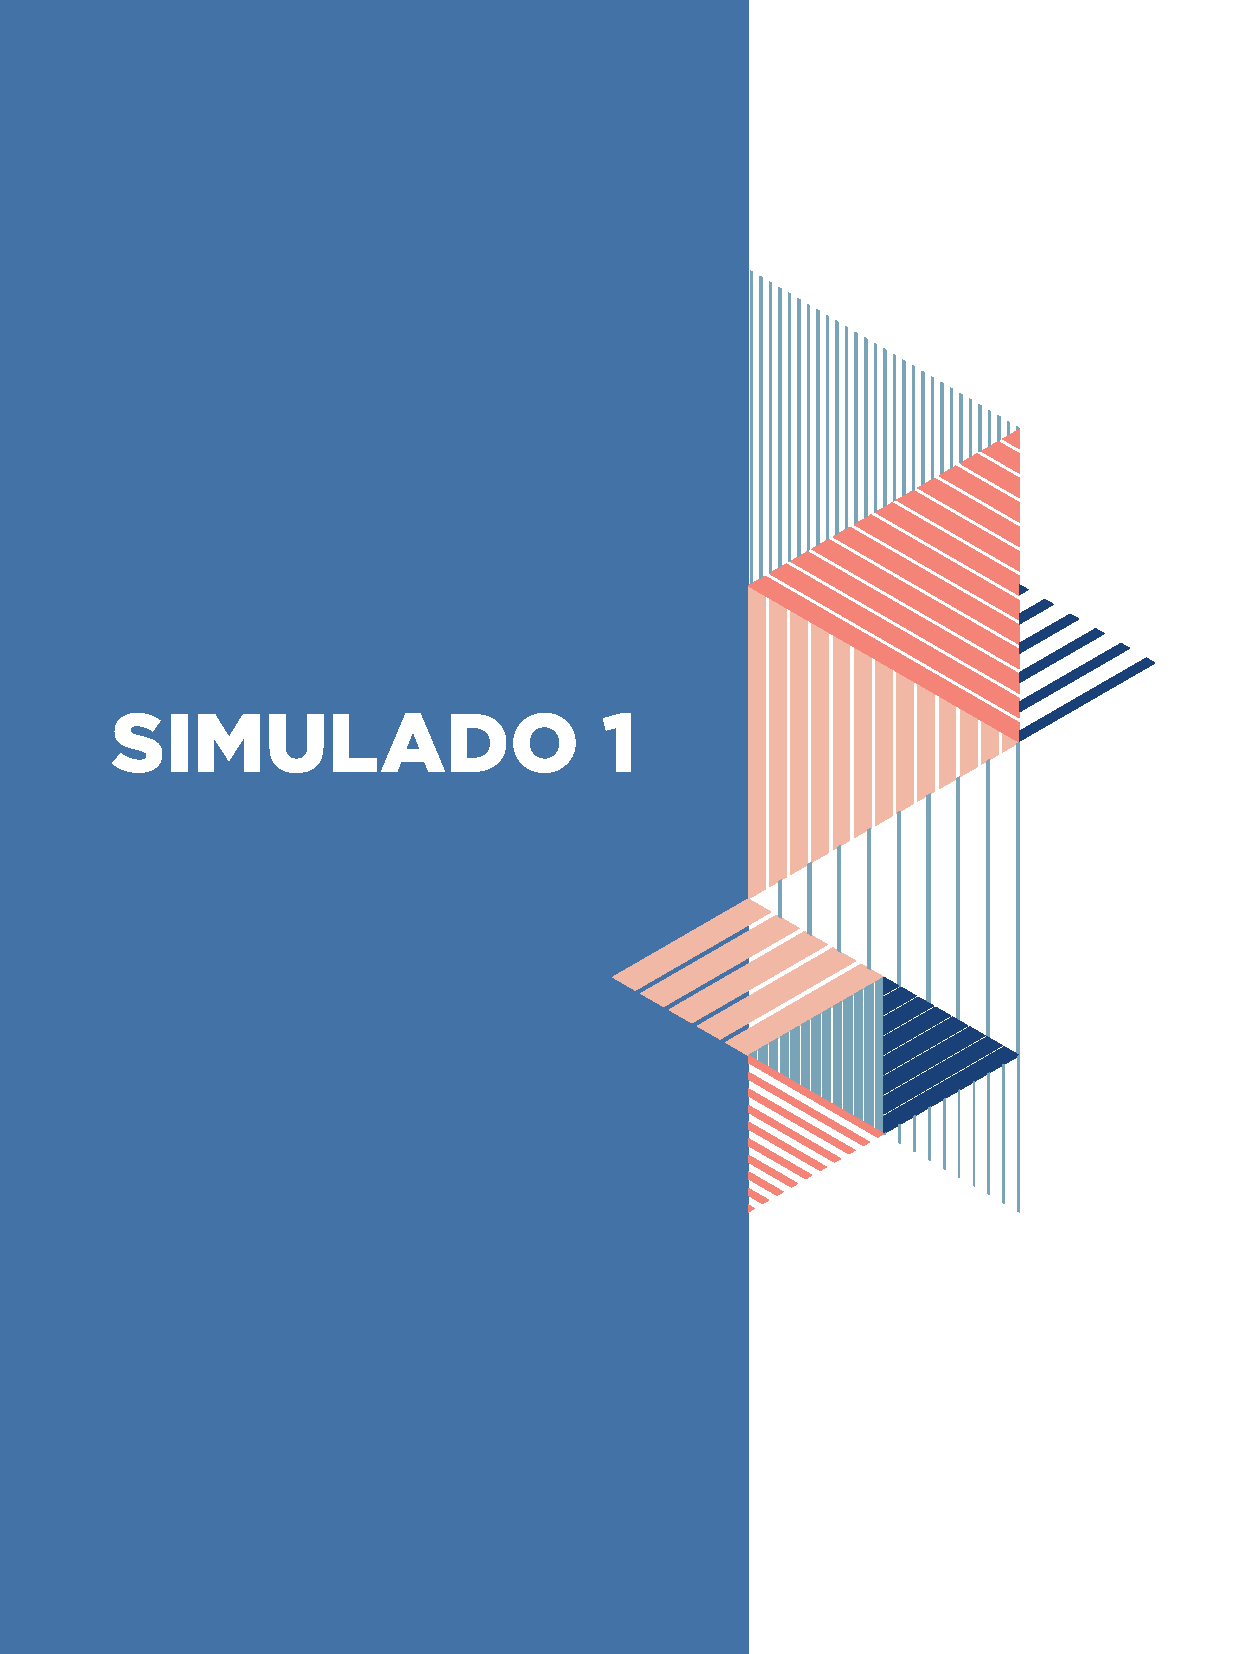
\includegraphics[scale=1]{../watermarks/1simulado9ano.pdf}
\end{figure}


\pagebreak


\section*{Simulado 1}

\num{1} Leia o texto a seguir.

\begin{figure}[H]
\centering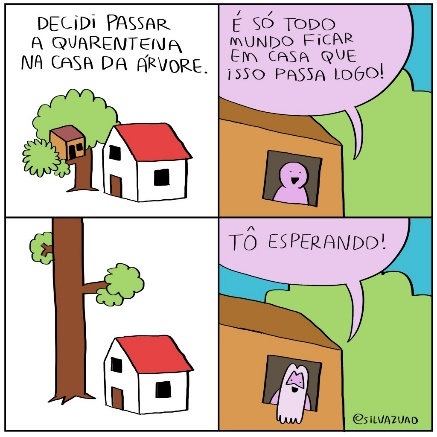
\includegraphics[width=\textwidth,height=1.98077in]{./imgSAEB_6_POR/media/image34.jpeg}
\end{figure}

\noindent No primeiro quadrinho da tira, o modalizador enunciativo promove a
intenção de:

\begin{escolha}
\item Certeza. 
\item Dúvida. 
\item Condição. 
\item Negação. 
\end{escolha}

%\paragraph{BNCC: EF69LP28}

% Gabarito, treino?
% \begin{escolha}
% \item A intenção é a de certeza.
% \item O modalizador em questão é o verbo decidi, que promove a intenção de
% certeza do enunciador.
% \item A intenção de condição aprece no segundo quadrinho, por meio do
% modalizador ``só'', quando o enunciador afirma que ``é só todo mundo
% ficar em casa que isso passa logo''.
% \item Em nenhum dos quadrinho há qualquer intenção de negação por parte do
% enunciador.
% \end{escolha}

\num{2} Leia a reportagem a seguir.

\begin{quote}
\centering\noindent\textbf{Sabores sem fronteiras}\\

\centering\noindent\emph{Livro com receitas de refugiados é um convite para conhecer
trajetórias de vida e sabores}\\

\noindent Ricardo nasceu em Caracas, o segundo de quatro irmãos. {[}\ldots{]} Ele
sempre prepara o \emph{sancocho} em sua casa no bairro do Butantã, em
São Paulo. ``Sempre cozinhei este prato quando Venezuela, na praia, em
reuniões com meus irmãos, primos, com música e cerveja. Fazer
\emph{sancocho} é como fazer uma festa'', contou. ``Fazer o prato aqui
no Brasil é importante porque assim posso compartilhar algo da minha
cultura'', disse.

\fonte{Patrícia Mariuzzo. Unicamp. Sabores sem fronteiras. Disponível em: https://www.unicamp.br/unicamp/ju/noticias/2022/02/07/sabores-sem-fronteiras.
Acesso em: 17 mar. 2023.}
\end{quote}

\noindent Ao dizer que ``fazer \emph{sancocho} é como fazer uma festa'', Ricardo,
o entrevistado, quer dizer que

\begin{escolha}
\item O prato só é feito quando há uma celebração.
\item O prato é sinônimo de alegria e comemoração na Venezuela.
\item Na Venezuela, o prato é feito tipicamente em festas e reuniões
familiares.
\item O prato traz boas memórias das reuniões familiares que ele tinha na
Venezuela.
\end{escolha}

%\paragraph{BNCC: EF69LP43}

% Gabarito, treino?
% \begin{escolha}
% \item Incorreta. O prato não é feito somente em celebrações. No texto mesmo
% é informado que Ricardo faz o prato no Brasil.
% \item Incorreta. O prato é sinônimo de boas lembranças para Ricardo, não
% necessariamente na Venezuela.
% \item Incorreta. Ricardo costumava fazer o prato em reuniões com seus
% familiares e amigos, mas o texto não informa que é tipicamente feito
% somente nessas ocasiões.
% \item Para Ricardo, o prato remete às boas memórias que tinha das reuniões
% com amigos e familiares na Venezuela, com música e cerveja.
% \end{escolha}

\num{3} Quando à escolha do título da matéria, ``Sabores sem fronteiras'',
refere-se

\begin{escolha}
\item à história de Ricardo.
\item às fronteiras entre um país e outro.
\item ao nome do livro mencionado no texto.
\item ao fato de tratar de alimentos do mundo todo.
\end{escolha}

%\paragraph{BNCC: EF67LP07}

% Gabarito, treino?
% \begin{escolha}
% \item Incorreta. O título não trata especificamente da história de Ricardo.
% Ele é apenas um exemplo.
% \item Incorreta. O título não trata apenas das fronteiras entre um país e
% outro, mas sim dos pratos de cada lugar que aparecem no livro.
% \item Incorreta. Não se pode afirmar que esse é o nome do livro.
% \item O título da matéria, ``Sabores sem fronteiras'', refere-se ao fato de
% o livro trazer receitas do mundo todo.
% \end{escolha}

\num{4} Observe uma imagem retirada do Twitter da Prefeitura do
município do Rio de Janeiro:

\begin{figure}[H]
\centering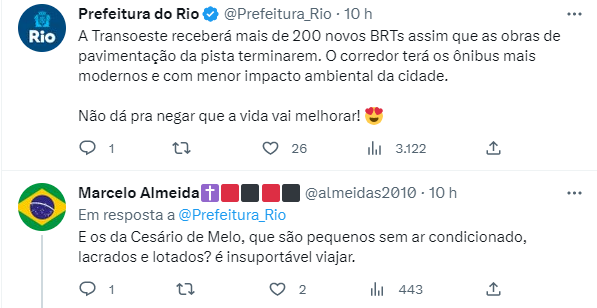
\includegraphics[width=4.97543in,height=2.56689in]{./imgSAEB_6_POR/media/image6.png}
\caption{Interface gráfica do usuário, Aplicativo Descrição gerada
automaticamente.}
\end{figure}

%Arte, por favor, borrar o nome da pessoa que comentou o Tweet da prefeitura.
% REVER
% \fonte{\href{https://twitter.com/Prefeitura_Rio/status/1633079144815681536}{https:\/\/twitter.com\/Prefeitura\_Rio/status1633079144815681536}}

\noindent Ao dizer que ``é insuportável viajar'', a pessoa que reclama sobre o
transporte utiliza uma figura de linguagem para representar seu
sentimento. Essa figura é:

\begin{escolha}
\item Hipérbole.
\item Metáfora.
\item Catacrese.
\item Personificação.
\end{escolha}

%\paragraph{BNCC: EF67LP38}

% Gabarito, treino?
% \begin{escolha}
% \item Correta. A pessoa utiliza uma hipérbole ao dizer que é insuportável
% viajar nos ônibus daquela linha, pois são pequenos e sem ar.
% \item Incorreta. Metáfora é uma comparação, o que não ocorre no comentário.
% \item Incorreta. Catacrese é uma figura de palavra que ocorre quando não há
% um termo específico para designar um conceito.
% \item Incorreta. Personificação é o ato de dar características humanas a
% seres e objetos inanimados.
% \end{escolha}

\num{5} Leia o texto a seguir.

\begin{quote}
\centering\noindent \textbf{O Brasil precisa do SUS: lançada campanha nacional de defesa do
Sistema Único de Saúde}\\
\medskip


\noindent A coordenadora do Campus Virtual Fiocruz, Ana Furniel, consoante com a
campanha \#OBrasilPrecisadoSUS, aponta que o Sistema Único de Saúde é
imprescindível para o país. Seu papel na pandemia ressaltou ainda mais a
sua importância. ``É interessante pensar no todo, pois quando falamos do
SUS ainda se pensa de forma limitada ao atendimento hospitalar. No
entanto, o SUS é maior, ele é atenção hospitalar, sim, mas é vacina,
medicamento, atenção primária, vigilância e é, especialmente para nós,
formação de profissionais de saúde. Essa é a esfera de contribuição do
CVF''.

\fonte{Isabela Schincariol. \emph{O Brasil precisa do SUS: lançada campanha
nacional de defesa do Sistema Único de Saúde}. Fiocruz, publicado em 15
de dez. 2020. Disponível em: https://campusvirtual.fiocruz.br/portal/?q=noticia/59976.
Acesso em: mar. 2023. Adaptado.}
\end{quote}

\noindent A palavra ``imprescindível'', usada pela especialista para defender
o SUS, poderia ser substituída, neste contexto, por

\begin{escolha}
\item Indispensável.
\item Irrecusável.
\item Incontestável.
\item Insustentável.
\end{escolha}

%\paragraph{BNCC: EF67LP04}

% Gabarito, treino?
% \begin{escolha}
% \item Imprescindível quer dizer que o SUS é absolutamente necessário, ou
% seja, indispensável.
% \item Incorreta. Irrecusável é a característica do que não se pode recusar,
% o que não é o caso do SUS no contexto.
% \item Incorreta. Incontestável é a característica do que não se contesta, o
% que não é o caso do SUS no contexto.
% \item Incorreta. Insustentável significa que o SUS não se manteria, não se
% sustentaria, o que não é o caso do contexto.
% \end{escolha}

\num{6} Leia o \emph{jingle} da campanha de Júlio Prestes, um homem que
foi candidato à presidência do Brasil em 1920:

\begin{verse}
Ó Seu Toninho\\
Da terra do leite grosso\\
Bota cerca no caminho\\
Que o paulista é um colosso
\end{verse}

\noindent O objetivo da música da campanha é:"

\begin{escolha}
\item Incentivar as pessoas a votarem.
\item Ressaltar as qualidades de Júlio Prestes.
\item Convidar seu Toninho a votar em Júlio Prestes.
\item Incentivar os paulistas a votarem em Júlio Prestes.
\end{escolha}

%\paragraph{BNCC: EF67LP04}

% Gabarito, treino?
% \begin{escolha}
% \item Incorreta. A canção não tem como objetivo incentivar as pessoas a
% votarem, mas sim de divulgar um candidato.
% \item Correta. A canção ressalta as qualidades do candidato, a fim de
% convencer as pessoas a votarem nele.
% \item Incorreta. Seu Toninho é um nome que representa o eleitor de modo
% geral.
% \item Incorreta. Apenas o candidato é paulista e não os eleitores de modo
% geral.
% \end{escolha}

\num{7} Leia os quadrinhos.

\begin{figure}[H]
\centering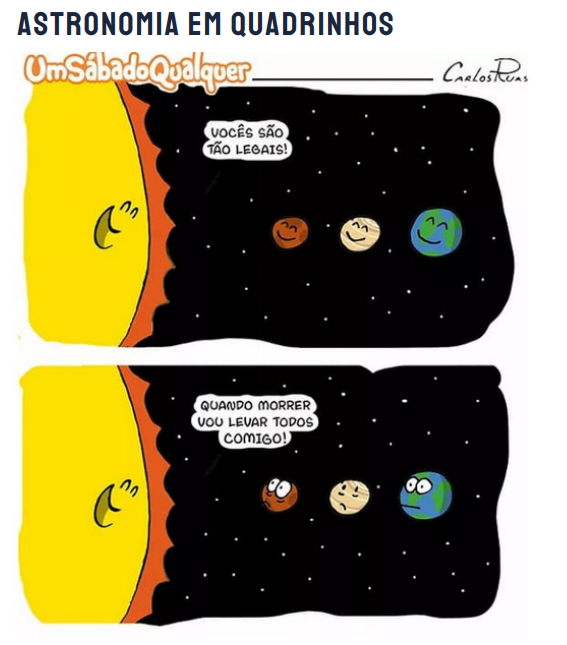
\includegraphics[width=4.75833in,height=5.41291in]{./imgSAEB_6_POR/media/image12.png}
\caption{Carlos Ruas.}
\end{figure}

\noindent O texto em quadrinhos foi usado para apresentar, em uma linguagem menos
técnica e mais acessível, um texto de divulgação científica que
explicaria:

\begin{escolha}
\item O que poderia apagar o Sol.
\item O que poderia extinguir a Terra.
\item O que aconteceria aos planetas se o Sol se apagasse.
\item De que forma a vida na Terra seria extinta se o Sol morresse.
\end{escolha}

%\paragraph{BNCC: EF69LP20}

% Gabarito, treino?
% \begin{escolha}
% \item Incorreta. O quadrinho não menciona o que poderia apagar o sol, e sim
% o que aconteceria aos outros astros se ele se apagasse.
% \item Incorreta. Embora o fim do Sol seja uma hipótese de extinção da vida
% na Terra, a temática do quadrinho são as consequências do apagão do Sol.
% \item Correta. O quadrinho explica, de forma lúdica, que sem o Sol nenhum
% planeta se manteria vivo, pois estão todos os três girando em torno do
% Sol.
% \item Incorreta. A extinção da vida na Terra poderia ser causada pelo
% apagão do sol, mas não é a única hipótese.
% \end{escolha}

\num{8} Observe o infográfico a seguir.

\begin{figure}[H]
\centering
\includegraphics[width=3.43333in,height=3.37681in]{./imgSAEB_6_POR/media/image15.jpeg}
\caption{Disponível em: https://aetrancoso.pt/2019/10/10/10-de-outubro-de-2019-dia-mundial-da-saude-mental.}
\end{figure}

\noindent Analisando-se os recursos verbais e não verbais, pode-se afirmar que o
público-alvo do infográfico é:

\begin{escolha}
\item Adultos.
\item Jovens e crianças.
\item Alunos de escolas públicas.
\item Adultos e idosos.
\end{escolha}

%\paragraph{BNCC: EF69LP16}

% Gabarito, treino?
% \begin{escolha}
% \item Incorreta. O texto pode ser consumido por adultos, mas não é o
% público-alvo.
% \item O infográfico apresenta imagens com traços leves e lúdicos, bem como
% uma fonte semelhante à letra cursiva. Esse tipo de imagem é mais comum
% em meios infanto-juvenis. Além disso, os textos são claros e dão pistas
% de que são destinados à pessoas mais vulneráveis, que precisam do apoio
% de um adulto, por exemplo.
% \item Incorreta. Qualquer jovem ou criança é o público do texto, não
% especificamente alunos de escolas públicas.
% \item Incorreta. A linguagem usada para alcançar adultos e idosos poderia
% ser mais formal e apresentar outros tipos de imagem, mais densas, por
% exemplo.
% \end{escolha}

\num{9} Leia o texto a seguir.

\begin{quote}
\noindent Apesar de nunca ter visto o lobo, Chapeuzinho Amarelo morria de medo
dele.

Um belo dia a menina encontrou o tal lobo que tanto temia, e para a
surpresa de todos, foi perdendo o medo e, o mais importante, o medo de
ter medo.

O lobo ficou ofendido de estar diante de uma menina que não tinha medo
dele: Ficou mesmo envergonhado, triste, murcho e branco-azedo, porque um
lobo, tirando o medo, é um arremedo de lobo. É feito um lobo sem pelo.
Lobo pelado.

\fonte{Chico Buarque. \emph{Chapeuzinho Amarelo}. Ilustrações de Ziraldo. Belo
Horizonte: Autêntica, 2017.}
\end{quote}

\noindent A obra \emph{Chapeuzinho Amarelo} apresenta intertextualidade com outra
história conhecida a partir do recurso de:

\begin{escolha}
\item Citação direta.
\item Citação indireta.
\item Paráfrase.
\item Citação de citação.
\end{escolha}

%\paragraph{BNCC: EF69LP43}

% Gabarito, treino?
% \begin{escolha}
% \item Incorreta. O autor não apresenta em sua obra trechos da obra original
% Chapeuzinho Vermelho.
% \item Incorreta. O autor não faz menção à obra original conhecida,
% Chapeuzinho Vermelho.
% \item Correta. Chapeuzinho Amarelo é a história de Chapeuzinho Vermelho
% recontada sob a perspectiva de Chico Buarque, portanto, pode-se dizer
% que é uma paráfrase.
% \item Incorreta. A história Chapeuzinho Amarelo não cita de nenhuma forma a
% obra original conhecida, Chapeuzinho Vermelho.
% \end{escolha}

% Saeb: Analisar efeitos de sentido produzido pelo uso de formas de
% apropriação textual (paráfrase, citação etc.).

\num{10} Leia o texto a seguir.

\begin{quote}
\noindent Ruth Rocha recebeu a equipe da TV Brasil em sua residência, em São
Paulo, para um papo sobre sua trajetória no universo literário e a
importância da leitura para as novas gerações.

Na entrevista, a escritora diz que é preciso conversar com as crianças
pois elas entendem mais do que se imagina. A autora conta que entende e
gosta de falar para as crianças de ontem e de hoje.

Ruth Rocha também destaca a importância do professor na formação do
público leitor. "O professor deve ler o livro antes e, se gostar, ler
para os alunos. Todos têm que gostar para dar certo", sugere a veterana
que adora ler e continua lendo de tudo.

Reverenciada pela crítica e pelo público, a autora foi reconhecida com
diversos prêmios como o Jabuti.

\fonte{Disponível em: https://tvbrasil.ebc.com.br/entrevista-com-ruth-rocha-e-destaques-no-dia-das-criancas. Acesso em: mar. 2023. Adaptado.}
\end{quote}

\noindent O trecho que representa uma opinião da entrevistada é:

\begin{escolha}
\item O professor deve ler o livro antes e, se gostar, ler para os alunos.
\item Ruth Rocha também destaca a importância do professor na formação do
público leitor.
\item \ldots{} a veterana que adora ler e continua lendo de tudo.
\item \ldots{} a autora foi reconhecida com diversos prêmios como o Jabuti.
\end{escolha}

%\paragraph{BNCC: EF67LP04}

% Gabarito, treino?
% \begin{escolha}
% \item Incorreta. O trecho representa uma verdade, segundo a especialista.
% \item Correta. Neste trecho fica implícito que o fato de o professor ser
% importante é uma opinião da autora.
% \item Incorreta. O trecho apresenta um fato sobre a autora.
% \item Incorreta. O trecho apresenta um fato sobre a autora.
% \end{escolha}

\num{11} Leia o texto a seguir.

\begin{quote}
\noindent E Chapeuzinho Amarelo, de tanto pensar no LOBO, de tanto sonhar com
LOBO, de tanto esperar o LOBO, um dia topou com ele que era assim: carão
de LOBO, olhão de LOBO, jeitão de LOBO e principalmente um bocão tão
grande que era capaz de comer duas avós, um caçador, rei, princesa, sete
panelas de arroz e um chapéu de sobremesa.

\fonte{BUARQUE, Chico. \emph{Chapeuzinho Amarelo}. Ilustrações de Ziraldo. Belo
Horizonte: Autêntica, 2017.}
\end{quote}

\noindent A repetição da palavra lobo, no trecho de \emph{Chapeuzinho Amarelo}, tem o
objetivo de:

\begin{escolha}
\item Remeter ao lobo da famosa história da Chapeuzinho Vermelho, que já
está na cabeça das pessoas.
\item Reforçar que tipo de animal a menina tinha estava pensando.
\item Provocar humor no modo como se pronuncia muitas vezes a palavra lobo.
\item Fazer com que o leitor pense tanto no lobo quando a Chapeuzinho
Amarelo.
\end{escolha}

%\paragraph{BNCC: EF67LP27}

% Gabarito, treino?
% \begin{escolha}
% \item Correta. O lobo que aparece neste trecho o um lobo presente na
% memória coletiva, consagrado pela história da Chapeuzinho Vermelho, o
% que se justifica pela descrição do animal.
% \item Incorreta. A ideia não era reforçar o animal em que ela estava
% pensando, e sim especificá-lo.
% \item Incorreta. Embora ocorra aliteração, o intuito do trecho não é
% provocar humor com essa figura de som.
% \item Incorreta. A ideia é fazer com que o leitor pense no lobo em que ela
% estava pensando, ou seja, o da Chapeuzinho Vermelho.
% \end{escolha}

\num{12} Observe a propaganda a seguir.

\begin{figure}[H]
\centering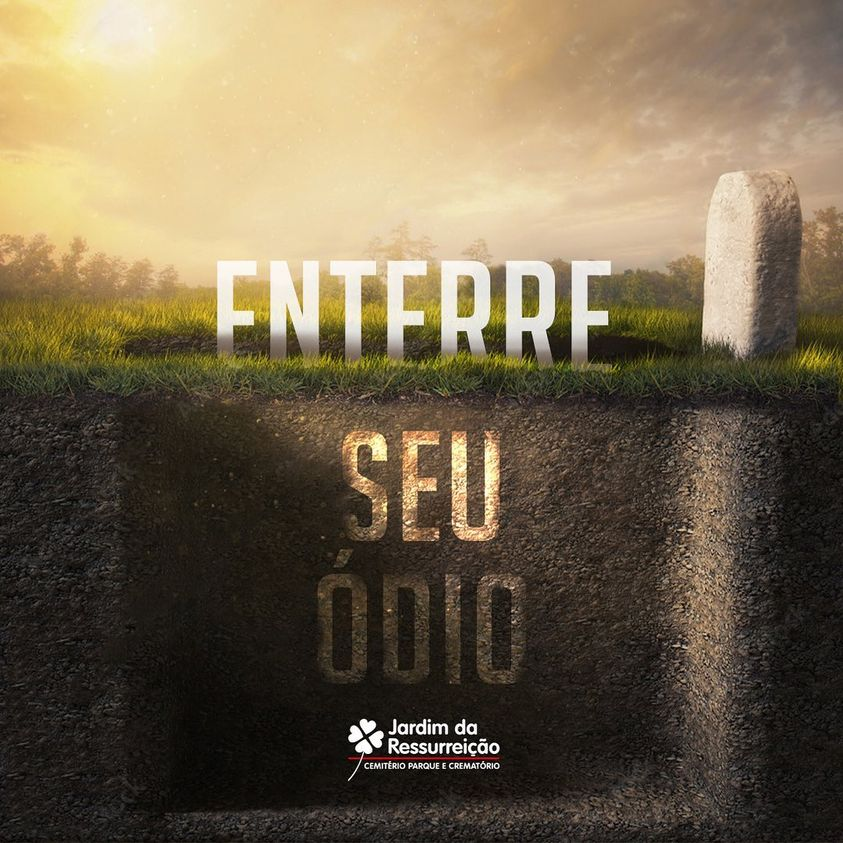
\includegraphics[width=4.65833in,height=4.65833in]{./imgSAEB_6_POR/media/image35.jpeg}
\end{figure}

\noindent O argumento utilizado na campanha para incentivar o combate ao discurso
de ódio é formado por

\begin{escolha}
\item Uma metáfora.
\item Um eufemismo.
\item Uma hipérbole.
\item Uma personificação.
\end{escolha}

%\paragraph{BNCC: EF67LP38}

% Gabarito, treino?
% \begin{escolha}
% \def\labelenumi{\alph{enumi})}
% \item Incorreta. A metáfora é uma comparação implícita entre duas coisas
% que têm características em comum.
% \item Correta. A campanha utiliza-se de um eufemismo, por meio da junção do
% recurso visual da cova (sentido literal) com o verbo enterrar (sentido
% conotativo), para dar o sentido de humor e argumentar contra o discurso
% de ódio.
% \item Incorreta. A hipérbole é um exagero proposital para enfatizar uma
% ideia ou emoção.
% \item Incorreta. A personificação é a atribuição de características humanas
% a seres inanimados ou animais.
% \end{escolha}

\num{13} Leia um trecho da crônica ``A bola!'', de Mario Prata.

\begin{quote}
\noindent Mas tente, agora, entender o mundo sem a bola. E o esporte. Acho que
fora o automobilismo, as lutas, a esgrima e o boxe, tudo gira em torno
da bola. Mesmo que seja uma bola na trave.

Desde a de pingue-pongue até a de basquete (que me parece ser a maior),
a bola é a bola e ninguém tasca. A bola com as mãos, com os pés, com a
cabeça e até com umas raquetes dando porradas nela. Sempre a bola.

Outra coisa interessante é que a bola não evolui. Nasceu bola e é bola
até hoje, ao contrário das rodas que hoje tem até com freio ABS. Tem até
roda gigante. Tem até programa de televisão com nome dela: Roda Viva.
Como se existisse uma roda morta.

\fonte{Mario Prata. ``A bola!''. Disponível em: https://marioprata.net/cronicas/a-bola. Acesso em: mar. 2023. Adaptado.}
\end{quote}

\noindent No trecho, notam-se claramente aspectos relacionados a variação
linguística:

\begin{escolha}
\item Cultural.
\item Histórico.
\item Social.
\item Estilístico.
\end{escolha}

%\paragraph{BNCC: EF69LP55}

% Gabarito, treino?
% \begin{escolha}
% \item Incorreta. As variações culturais ocorrem de acordo com a cultura dos
% falantes, e muitas vezes estão relacionadas a aspectos geográficos.
% \item Correta. As variações históricas tratam das mudanças ocorridas na
% língua com o decorrer do tempo. O texto nitidamente foi escrito décadas
% atrás, o que se pode notar pelo uso de palavras já ultrapassadas, como
% tasca, e a menção ao programa Roda Viva no presente, como se ainda
% existisse.
% \item Incorreta. As variações sociais são as diferenças de acordo com o
% grupo social do falante, como profissão, faixa etária, entre outros.
% \item Incorreta. As variações estilísticas remetem ao contexto que exige a
% adaptação da fala ou ao estilo dela.
% \end{escolha}

\num{14} Leia o texto a seguir.

\begin{figure}[H]
\centering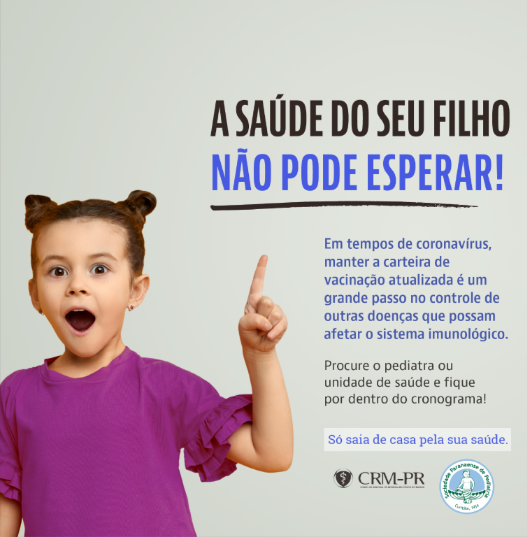
\includegraphics[width=4.23378in,height=4.3141in]{./imgSAEB_6_POR/media/image36.png}
\caption{Disponível em: https://www.crmpr.org.br/Pais-precisam-manter-atualizado-o-calendario-de-vacinacao-dos-filhos-mesmo-na-pandemia-11-54287.shtml}
\end{figure}

\noindent Considerando o pronome ``seu'' no título da campanha, qual é o público
alvo da campanha?

\begin{escolha}
\item Pediatras.
\item Público de modo geral.
\item Crianças em idade de Vacinação.
\item Pais e responsáveis de crianças em idade de vacinação.
\end{escolha}

%\paragraph{BNCC: EF06LP12}

% Gabarito, treino?
% \begin{escolha}
% \item Incorreta. Embora as crianças sejam os pacientes de pediatras, a
% campanha deixa claro que não se referem a ``seus pacientes'', mas sim
% ``seus filhos''
% \item Incorreta. O público de modo geral não necessariamente possui filhos.
% \item Incorreta. Embora a vacina se destine às crianças, a campanha se
% dirige aos seus pais.
% \item ``Seu'' é um pronome possessivo que se refere aos filhos das pessoas
% às quais a campanha é dirigida
% \end{escolha}

\num{15} Leia o texto.

\begin{quote}
\noindent Dez anos atrás, o trabalho de uma arqueóloga da USP fez história ao
examinar, pela primeira vez, os restos mortais dos primeiros imperadores
do Brasil — incluindo D.\,Pedro I e suas duas consortes, as
imperatrizes D.\,Leopoldina e D.\,Amélia. Agora, um novo capítulo dessa
pesquisa chega à era digital ilustrada com uma sofisticada coleção de
retratos virtuais desses três personagens cruciais da história
brasileira.

Os retratos foram construídos por um artista digital com base em
evidências anatômicas, históricas e arqueológicas, compiladas pela
equipe que analisou o conteúdo das tumbas imperiais. ``É uma fusão de
ciência e arte'', diz a arqueóloga e historiadora Valdirene Ambiel,
responsável pelo projeto. O trabalho foi realizado para a sua tese de
doutorado no Departamento de Patologia da Faculdade de Medicina da USP,
sob orientação do professor Carlos Augusto Pasqualucci.

``O principal legado que eu espero que essa pesquisa traga é que as
pessoas hoje, do século 21, possam olhar para esses personagens
históricos do século 19 como seres humanos, que é o que eles realmente
eram. Da mesma forma como nós temos a nossa vida hoje, eles tiveram a
vida deles no passado'', diz Valdirene Ambiel.

\fonte{Herton Escobar. Cara a cara com a família imperial: pesquisa simula
rostos de D.\,Pedro I e suas esposas. Jornal da USP, publicado em
07 mar. 2023. Atualizado em 10 mar. 2023. Disponível em: https://jornal.usp.br/ciencias/cara-a-cara-com-a-familia-imperial-pesquisa-simula-rostos-de-d-pedro-i-e-suas-esposas.
Acesso em: 14 mar. 2023. Adaptado.}
\end{quote}

\noindent A pesquisadora justifica sua pesquisa a partir do argumento de que:

\begin{escolha}
\item As pessoas não têm noção de como eram os membros da família Real.
\item As pessoas não acreditam na existência da família Real.
\item É importante examinar, pela primeira vez, os restos mortais dos
primeiros imperadores do Brasil.
\item É importante saber que as pessoas da família Real tinham vida como
nós temos hoje em dia.
\end{escolha}

%\paragraph{BNCC: EF67LP05}

% Gabarito, treino?
% \begin{enumerate}
% \item Incorreta. O texto não deixa claro o conhecimento das pessoas em
% geral sobre a aparência da família Real, porém, não é isso que a
% pesquisadora usa para justificar a pesquisa.
% \item Incorreta. Em nenhum momento o texto menciona que pessoas não
% acreditam na existência da família Real.
% \item Incorreta. A pesquisadora examinou os restos mortais dos membros da
% família Real no intuito de desenvolver sua pesquisa, e não porque é
% importante fazer isso.
% \item Correta. Segundo a pesquisadora, o principal legado da pesquisa é
% fazer com que esses personagens históricos do século 19 sejam vistos
% como pessoas como nós, o que realmente eram, e que tinham a vida deles
% no passado.
% \end{enumerate}

\num{16} Veja a imagem.

\begin{figure}[H]
\centering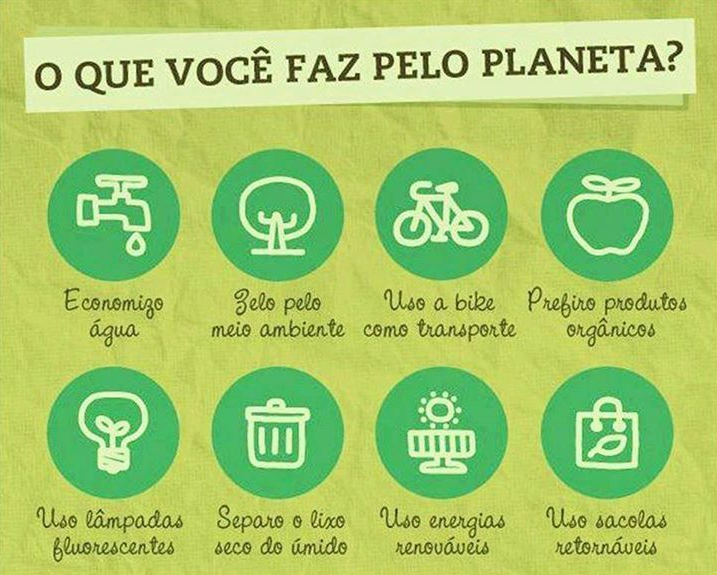
\includegraphics[width=5.90556in,height=4.73611in]{./imgSAEB_6_POR/media/image37.png}
\caption{Disponível em: https://www.esteio.rs.leg.br/institucional/noticias/cartazes-propoem-conscientizacao-ambiental-nas-escolas-de-esteio.}
\end{figure}

\noindent O infográfico é uma ferramenta que serve para transmitir informações
através do uso de imagens, desenhos e demais elementos visuais gráficos.
Normalmente o infográfico acompanha um texto que fala sobre um assunto
correlato. O texto que acompanharia o infográfico acima teria como tema
central:

\begin{escolha}
\item Consumo consciente.
\item Desmatamento.
\item Riscos ao planeta.
\item Dicas de ecologia.
\end{escolha}

%\paragraph{BNCC: EF69LP02}

% Gabarito, treino?
% \begin{escolha}
% \item Correta. O infográfico traz dicas de consumo consciente de modo
% geral, que impactam no bem-estar de todos no planeta.
% \item Incorreta. O infográfico traz dicas variadas de como zelar pelo
% planeta, e não por florestas especificamente.
% \item Incorreta. Embora o consumo desenfreado e inconsequente ocasione
% sérios riscos ao planeta, a temática tratada no infográfico é consumo
% consciente.
% \item Incorreta. O infográfico não fala apenas de ecologia, e sim de
% consumo consciente.
% \end{escolha}

\pagebreak

\mbox{}

\begin{figure}
\vspace*{-3cm}
\hspace*{-3.7cm}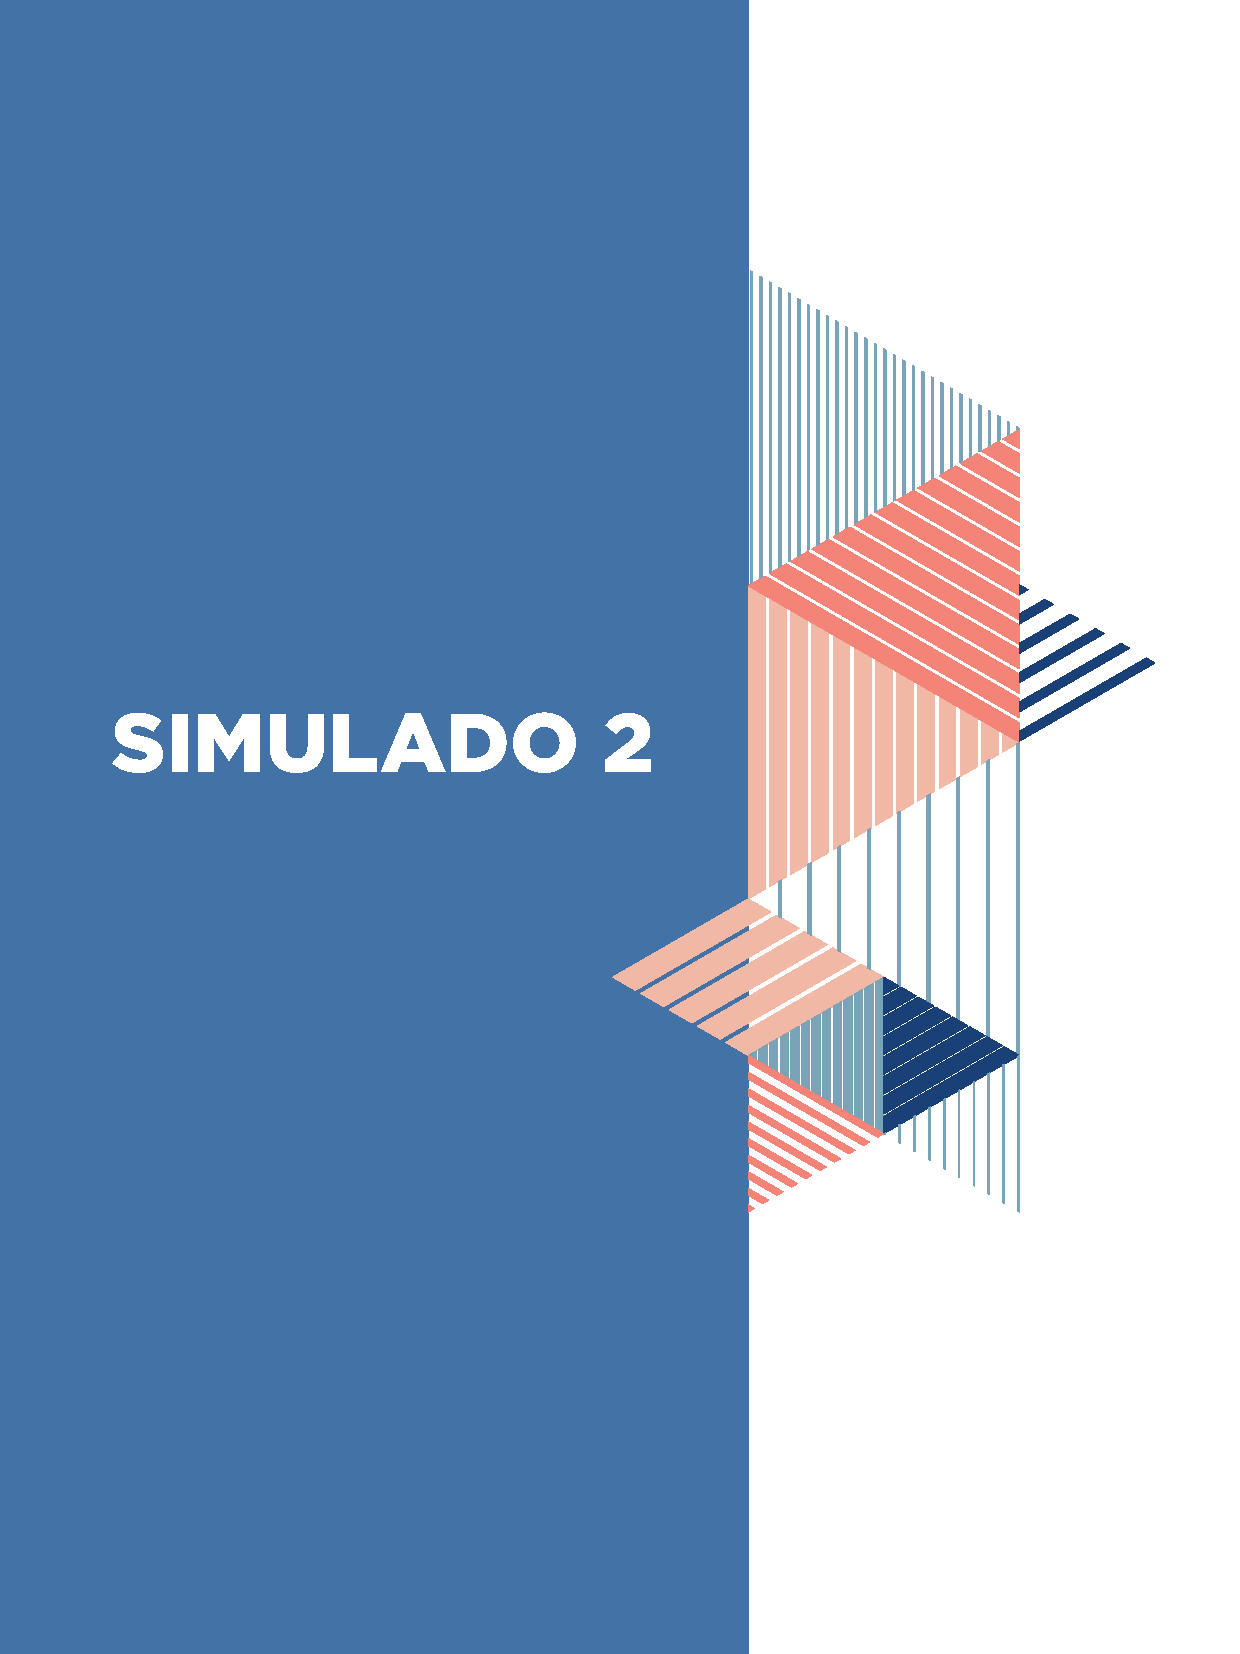
\includegraphics[scale=1]{../watermarks/2simulado9ano.pdf}
\end{figure}


\pagebreak

\section*{Simulado 2}

\num{1} Leia o texto a seguir.

\begin{figure}[H]
\centering
\includegraphics[width=5.90556in,height=3.95694in]{./imgSAEB_6_POR/media/image38.png}
\caption{Disponível em: http://www.unifap.br/conscientizacao-no-transito-e-o-objetivo-da-campanha-maio-amarelo-2/.}
\end{figure}

\noindent A proposta da campanha é incentivar as pessoas a:

\begin{escolha}
\item ficar em casa.
\item sair apenas se necessário.
\item higienizar as mãos.
\item respeitar as leis de trânsito.
\end{escolha}

%\paragraph{BNCC: EF67LP07}

% Gabarito, treino?
% \item Incorreto. Como a campanha foi produzida em época de pandemia, a
% hashtag \#fiqueemcasa incentivava as pessoas a não saírem, porém, este
% não é o objetivo da campanha.
% \item Incorreta. A campanha orienta as pessoas as saírem apenas se
% necessário, mas o objetivo é respeitar as leis de trânsito.
% \item Incorreta. A campanha incentiva as pessoas a respeitarem as leis de
% trânsito. Como foi veiculada em época de pandemia, o texto menciona sair
% de casa apenas se necessário.
% \item Correta. A campanha é uma iniciativa da Polícia Rodoviária Federal e
% visa incentivar as pessoas a respeitarem as leis de trânsito.

\num{2} Leia o texto a seguir.

\begin{quote}
\centering\noindent\textbf{Damiani pede manutenção asfáltica em ruas esburacadas de
Sorriso}


\noindent Ouvir as necessidades da população e buscar encaminhamento para solução
dessas demandas também faz parte dos trabalhos do Poder Legislativo.
Nesta quarta-feira (23), o presidente da Câmara de Sorriso, vereador
Leandro Damiani, percorreu ruas e avenidas da Zona Leste do município,
região que concentra boa parte das reclamações referentes a buracos e
acúmulo de água nas vias públicas.

``A população está nos pedindo a manutenção do asfalto de várias ruas e
avenidas, entre elas a Travessa São Severino, onde estive nesta manhã.
Na visita pude observar que estas ruas são o retrato de muitas outras
paralelas que apresentam o mesmo, ou pior estado, de um asfalto
precário'', ressaltou o parlamentar.

De acordo com Damiani, uma indicação pedindo operações tapa-buraco no
município serão apresentadas por ele na próxima sessão e adianta que irá
se reunir com representantes do Executivo para debater o assunto.

\fonte{Câmara Municipal de Sorriso, publicado em nov.
2022. Disponível em: \emph{https://sorriso.mt.leg.br/noticia/damiani-pede-manutencao-asfaltica-em-ruas-esburacadas-de-sorriso-637e35ae893b7}.
Acesso em: mar. 2023.}
\end{quote}

\noindent A notícia apresenta uma reclamação:

\begin{escolha}
\item Do Poder Legislativo, referentes a buracos e acúmulo de água nas vias
pública.
\item Da população, sobre manutenção do asfalto de várias ruas e avenidas.
\item Do vereador, sobre pedindo operações tapa-buraco no município.
\item Dos representantes do Executivo, sobre a manutenção do asfalto.
\end{escolha}

%\paragraph{BNCC: EF67LP17}

% Gabarito, treino?
% \begin{escolha}
% \item Incorreta. É parte do trabalho do Legislativo buscar a solução para
% as demandas.
% \item A notícia trata da reclamação da população sobre manutenção do
% asfalto de várias ruas e avenidas de Sorriso. Damiani, o vereador,
% apenas é o porta-voz entrevistado.
% \item Incorreta. O vereador é o porta-voz dos pedidos da população.
% \item Incorreta. O vereador ficou encarregado de apresentar as demandas
% para o Executivo.
% \end{escolha}

\num{3} Observe a imagem a seguir.

\begin{figure}[H]
\centering\includegraphics[width=4.86098in,height=3.28333in]{./imgSAEB_6_POR/media/image39.png}
\end{figure}

\noindent O que provoca o efeito de humor da charge é:

\begin{escolha}
\item O fato de a mãe se emocionar com o filho.
\item A mãe estar sensibilizada com o presente caro.
\item O fato de o presente caro ser um botijão de gás.
\item O filho presentear a mãe com um presente incomum.
\end{escolha}

%\paragraph{BNCC: EF69LP03}

% Gabarito, treino?
% \begin{escolha}
% \item Incorreta. A mãe se emociona com o presente do filho.
% \item Incorreta. A mãe se emociona com o tipo de presente caro.
% \item O humor da tira é o fato de o presente ser um botijão de gás que, de
% tão caro, emocionou a mãe.
% \item Incorreta. O presente é incomum, mas aqui especificamente o humor
% está no fato de ser um botijão de gás, que custa muito caro.
% \end{escolha}

\num{4} Leia um trecho da obra ``O diário da princesa'', de Meg Cabot.

\begin{quote}
\centering\noindent\textbf{Terça-feira, 23 de setembro}\\

\noindent Às vezes, parece que tudo que faço é mentir.
Mamãe acha que estou reprimindo meus sentimentos sobre isso.
Eu digo a ela: ``Não, mamãe, não estou. Acho que é realmente bacana.
Enquanto você for feliz, eu serei feliz.''
Mamãe respondeu: ``Eu não acho que você esteja sendo honesta comigo.''
Em seguida, ela me deu este livro. Diz que quer que eu escreva nele meus
sentimentos, já que, diz ela, obviamente eu não acho que posso falar com ela sobre eles.
Ela quer que eu escreva sobre meus sentimentos?
Tudo bem, vou dizer, por escrito, quais são meus sentimentos.
\textsc{eu não posso acreditar que ela esteja fazendo isso comigo!}

\fonte{Meg Cabot. \emph{O diário da princesa}. Rio de Janeiro: Record, 2005. Fragmento.}
\end{quote}

\noindent A personagem principal da obra é Mia, uma adolescente comum que descobre
que é uma princesa de verdade, herdeira de um trono na Europa. O trecho
apresentado contextualiza o leitor com relação:

\begin{escolha}
\item À personalidade da personagem principal.
\item Ao tempo cronológico da história.
\item Aos personagens secundários da história.
\item Ao lugar em que acontece a história.
\end{escolha}

%\paragraph{BNCC: EF69LP47}

% Gabarito, treino?
% \begin{enumerate}
% \item O trecho contextualiza o leitor com relação à personalidade de Mia: o
% que ela pensa, como ela pensa e os dilemas pelos quais ela está
% passando.
% \item Incorreta. O trecho não deixa claro o tempo cronológico, embora o
% diário seja datado. Essa informação só é percebida no decorrer da obra.
% \item Incorreta. O trecho não apresenta personagens secundários, apenas Mia
% falando sobre a mãe.
% \item Incorreta. O trecho não apresenta o local onde acontece a história.
% \end{enumerate}

%Saeb: Analisar elementos constitutivos de textos pertencentes ao domínio
%literário.

\num{5} Analise o anúncio.

\begin{figure}[H]
\centering\includegraphics[width=4.26392in,height=4.23333in]{./imgSAEB_6_POR/media/image40.jpeg}
\caption{Disponível em: https://turismoemfoco.com.br/v1/2019/05/03/elba-ramalho-vira-garota-propaganda-do-maior-sao-joao-do-mundo.}
\end{figure}

\noindent Na propaganda, a expressão ``prepare seu coração'' é uma maneira
conotativa de orientar a pessoa a:

\begin{escolha}
\item Apaixonar-se pela festa de São João.
\item Controlar a ansiedade para a festa de São João.
\item Preparar-se fisicamente para a festa de São João.
\item Fazer um check up de saúde antes de ir para a festa de São João.
\end{escolha}

%\paragraph{BNCC: EF06LP12}

% Gabarito, treino?
% \begin{escolha}
% \item Incorreta. Embora o coração quase sempre esteja ligado à paixão,
% neste contexto ele está relacionado à ansiedade.
% \item A expressão ``prepare seu coração'' está relacionada à sensação de
% palpitação causada pela ansiedade.
% \item Incorreta. Como o próprio enunciado explica, a expressão é usada em
% sentido conotativo, ou seja, não literal.
% \item Incorreta. Como o próprio enunciado explica, a expressão é usada em
% sentido conotativo, ou seja, não literal.
% \end{escolha}

\num{6} Veja a imagem a seguir.

\begin{figure}[H]
\centering\includegraphics[width=5.19864in,height=5.50077in]{./imgSAEB_6_POR/media/image41.png}
\caption{Disponível em: https://dragoesdegaragem.com/cientirinhas/cientirinhas-18.}
\end{figure}

\noindent Qual das alternativas melhor descreve o tom da linguagem usada no texto?

\begin{escolha}
\item Nervoso e combativo.
\item Humorístxico e leve.
\item Sério e informativo.
\item Triste e melancólico.
\end{escolha}

%\paragraph{BNCC: EF69LP05}

% Gabarito, treino?
% \begin{escolha}
% \item Incorreta. Embora os macacos aparentemente estivessem discutindo no
% primeiro quadrinho, a linguagem é humorística e leve.
% \item Correta. O texto adota uma linguagem leve e humorística.
% \item Incorreta. O terceiro quadrinho propõe uma fala mais informativa da
% personagem, mas a tira é de humor.
% \item Incorreta. Em nenhum momento o texto aparenta qualquer indício de
% tristeza ou melancolia.
% \end{escolha}

\num{7} Leia o texto.

\begin{quote}
\noindent \emph{Quarta-feira, 18 de janeiro}

\noindent Estamos na Boa Vista e fomos hoje à casa de uns amigos que eram tão bons
para nós, todas as vezes que aqui vínhamos. Obsequiavam sempre a mamãe
com frutas, ovos, frangos e verduras.

Esta amizade ficou forte com a parecença de Luisinha, minha irmã, com a
sobrinha deles que estava fora. A mulher, Dona Mariquinha, dizia sempre
que nos via: ``Que saudades da Quitinha! Vendo a sua menina, parece que
estou vendo a outra, Dona Carolina. É cara duma, cara doutra, sem tirar
nem pôr. Ainda hei de juntar as duas para a senhora ver''. Mamãe dizia:
``É pena mesmo a sua não estar aqui''. Ela dizia: ``O dia chegará, Dona
Carolina.

\fonte{Helena Morley. \emph{Minha vida de menina}. 1ª ed. São Paulo: Companhia de Bolso, 2016.}
\end{quote}

\noindent O trecho ``Obsequiavam sempre a mamãe com frutas, ovos, frangos e
verduras'' apresenta qual tipo de variação linguística?

\begin{escolha}
\item Econômica 
\item Histórica 
\item Social 
\item Geográfica
\end{escolha}

%\paragraph{BNCC: EF69LP44}

% Gabarito, treino?
% \begin{escolha}
% \item Incorreta. O trecho e a forma de se expressar não tem relação com a
% classe econômica dos personagens envolvidos, mas sim com o período
% histórico em que o texto foi criado
% \item Correta. O texto original foi criado em meados de 1940, e por isso,
% retrata a variação linguística histórica, com palavras mais rebuscadas.
% Por exemplo: Obsequiava, que no contexto quer dizer presentear.
% \item Incorreta. O trecho e a forma de se expressar não tem relação com a
% contexto social dos personagens envolvidos, mas sim com o período
% histórico em que o texto foi criado
% \item Incorreta. O trecho e a forma de se expressar não tem relação com a
% origem geográfica dos personagens envolvidos, mas sim com o período
% histórico em que o texto foi criado
% \end{escolha}

\num{8} Leia o texto.

\begin{quote}
\noindent Dez anos atrás, o trabalho de uma arqueóloga da USP fez história ao
examinar, pela primeira vez, os restos mortais dos primeiros imperadores
do Brasil — incluindo D. Pedro I e suas duas consortes, as
imperatrizes D. Leopoldina e D. Amélia. Agora, um novo capítulo dessa
pesquisa chega à era digital ilustrada com uma sofisticada coleção de
retratos virtuais desses três personagens cruciais da história
brasileira.

Os retratos foram construídos por um artista digital com base em
evidências anatômicas, históricas e arqueológicas, compiladas pela
equipe que analisou o conteúdo das tumbas imperiais. ``É uma fusão de
ciência e arte'', diz a arqueóloga e historiadora Valdirene Ambiel,
responsável pelo projeto. O trabalho foi realizado para a sua tese de
doutorado no Departamento de Patologia da Faculdade de Medicina da USP,
sob orientação do professor Carlos Augusto Pasqualucci.

\fonte{Herton Escobar. \emph{Cara a cara com a família imperial: pesquisa simula
rostos de D. Pedro I e suas esposas}. Jornal da USP, publicado em
07 mar. 2023. Atualizado em 10 mar. 2023. Disponível em: https://jornal.usp.br/ciencias/cara-a-cara-com-a-familia-imperial-pesquisa-simula-rostos-de-d-pedro-i-e-suas-esposas. Acesso em: 14 mar. 2023. Adaptado.}
\end{quote}

\noindent Qual é a ideia central do texto?

\begin{escolha}
\item Contar a história de D. Pedro e da família Real brasileira.
\item Divulgar o trabalho de pesquisa de uma arqueóloga brasileira.
\item Explicar um fenômeno científico e artístico.
\item Fazer uma resenha de uma pesquisa científica.
\end{escolha}

%\paragraph{BNCC: EF69LP20}

% Gabarito, treino?
% \begin{escolha}
% \def\labelenumi{\alph{enumi})}
% \item Incorreta. A pesquisa é da arqueóloga que é sobre a família Real
% brasileira.
% \item O trecho é um texto de divulgação científica cujo objetivo é
% apresentar um trabalho de pesquisa e seus resultados.
% \item Incorreta. O texto tem a intenção de divulgar um trabalho de pesquisa
% e seus resultados.
% \item Incorreta. O texto de divulgação científica é informativo, e não
% opinativo.
% \end{escolha}

\num{9} Leia os textos a seguir.

\begin{quote}
\noindent\textbf{Texto 1}\quad ``— Adeus — disse a raposa. — Eis o meu segredo. É muito simples: só se vê bem com o coração. O essencial é invisível para os olhos.''

\fonte{\emph{O pequeno príncipe}.}

\noindent\textbf{Texto 2}\quad ``A grandeza não está em ser forte, mas no uso correto da força. Grande é aquela cuja força conquista mais corações.''

\fonte{\emph{Extraordinário}.}
\end{quote}

\noindent A mensagem que caracteriza a intertextualidade entre as duas obras é:

\begin{escolha}
\item Sempre siga seus sonhos. 
\item Seja gentil com as pessoas. 
\item Não deixe
de ter esperança. 
\item Aprenda com seus erros.
\end{escolha}

%\paragraph{BNCC: EF67LP27}

% Gabarito, treino?
% \begin{escolha}
% \item Incorreta. Os trechos não incentivam o leitor a buscar seus sonhos.
% \item Correta. Tanto no trecho de ``O pequeno príncipe'' quando no trecho
% de ``Extraordinário'' a mensagem que se passa é de uma relação gentil
% com as pessoas, a fim de conquistá-las.
% \item Incorreta. Os trechos falam de relações de afeto, e não de esperança.
% \item Incorreta. Os trechos não dão lição de moral relacionada a
% aprendizado com os erros.
% \end{escolha}

\num{10} Leia o texto a seguir.

\begin{quote}
\noindent Estudantes que ingressaram no ensino médio em 2022 frequentam as aulas
em um novo sistema, chamado de ``novo ensino médio'': esse novo formato
adotado pelas escolas levantou muitas opiniões divergentes,
principalmente por parte de estudantes, já que em algumas escolas o
ensino em tempo integral foi aplicado, os alunos tendem a se desenvolver
mais no tempo integral, com as 9 aulas diárias. Em meu ponto de vista
como estudante, o novo ensino médio assustou bastante no começo, mas a
coordenação da minha escola fez com que tudo ficasse mais leve. Foi
possível que nós nos adaptássemos ao longo dos meses — no começo foi
bastante difícil e confuso, eram 27 disciplinas e, mesmo que nem todas
tenham aulas massivas e sim aulas práticas, ainda assim era tudo muito
novo para nós que ficamos bastante tempo sem frequentar a escola.

\fonte{Grazi Dantas. O novo Ensino Médio na visão de uma estudante. Agência
Jovem de Notícias, publicado em out. 2022. Disponível em: https://agenciajovem.org/opiniao-o-novo-ensino-medio-na-visao-de-uma-estudante. Acesso em: mar. 2023. Adaptado.}
\end{quote}

\noindent Qual é o ponto de vista da autora sobre o novo Ensino Médio?

\begin{escolha}
\item
  Positiva, pois a escola tornou tudo mais leve.
\item
  Confusa, pois eram 27 disciplinas e tudo muito novo.
\item
  Negativa, pois o novo formato assustou bastante.
\item
  Positiva em alguns pontos e negativa em outros.
\end{escolha}

%\paragraph{BNCC: EF69LP16}

% Gabarito, treino?
% \begin{escolha}
% \item
%   Como a própria estudante informa, ``o novo ensino médio assustou
%   bastante no começo, mas a coordenação da minha escola fez com que tudo
%   ficasse mais leve''.
% \item
%   Incorreta. Embora fossem muitas disciplinas, a escola auxiliou os
%   estudantes e tudo ficou mais leve.
% \item
%   Incorreta. A estudante achou confuso de início, mas gostou da
%   proposta.
% \item
%   Incorreta. A estudante menciona dificuldades no início, mas acabou
%   gostando da proposta.
% \end{escolha}

\num{11} Leia o texto a seguir.

\begin{quote}
\noindent A popularização dos drones comerciais, das inteligências artificiais e
dos softwares de modelagem 3D permitiram o desenvolvimento de um novo
método para controlar áreas de reflorestamento. Durante seu doutorado no
Instituto de Energia e Ambiente (IEE) da USP, o engenheiro florestal e
pesquisador Rafael Walter de Albuquerque criou um procedimento mais
rápido e capaz de enriquecer os tradicionais.{[}\ldots{}{]} ``Toda
restauração demanda um monitoramento. Assim como nós temos que monitorar
o nosso organismo, que é complexo,— temos que fazer exames
periodicamente, principalmente quando a idade avança, para garantir que
está tudo em ordem —, quando nós estamos recuperando a floresta,
precisamos visitá-la periodicamente para ver se os dados dela estão bons
e se será preciso tomar uma atitude ou não'', conta Rafael Albuquerque
ao Jornal da USP.{[}\ldots{}{]}

\fonte{Ivan Conterno. ``Drones e modelagem 3D auxiliarão a recuperação de
florestas''. Jornal da USP, publicado em mar. 2023. Disponível em: https://jornal.usp.br/ciencias/drones-e-modelagem-3d-auxiliarao-a-recuperacao-de-florestas. Acesso em: mar. 2023. Adaptado.}
\end{quote}

\noindent Qual é o objetivo do pesquisador ao dizer que a floresta é como nosso
organismo, complexo?

\begin{escolha}
\item Promover uma evidência para apoiar um argumento.
\item Facilitar a compreensão do leitor por meio de uma metáfora.
\item Criar uma imagem vívida de uma floresta na mente do leitor.
\item Tornar o texto mais interessante para o leitor.
\end{escolha}

%\paragraph{BNCC: EF69LP43}

% Gabarito, treino?
% \begin{escolha}
% \item
%   Incorreta. Embora no trecho o objetivo seja apresentar um argumento
%   para a tese de que é necessário o uso do drone, o pesquisador o
%   compara a floresta ao organismo humano a fim de facilitar a
%   compreensão do leitor.
% \item
%   Correta. Para facilitar o entendimento do leitor quanto à importância
%   do drone para o reflorestamento, o pesquisador usa uma metáfora,
%   comparando a floresta ao nosso organismo.
% \item
%   Incorreta. O intuito é facilitar a compreensão do leitor, e não apenas
%   gerar uma imagem da floresta na mente dele.
% \item
%   Incorreta. O texto, por ser uma artigo de divulgação científica,
%   naturalmente é interessante para quem o lê pois o público-alvo com
%   frequência são pessoas que têm afinidade com o assunto.
% \end{escolha}

\num{12} Veja a imagem.

% REVER
\centering\includegraphics[width=5.90556in,height=4.96042in]{./imgSAEB_6_POR/media/image42.png}
%Uma imagem contendo Desenho técnico Descrição gerada automaticamente}

\noindent Em qual momento da história é apresentado o efeito de humor?

\begin{escolha}
\item
  No primeiro quadrinho, que já apresenta um cliente bem incomum.
\item
  No segundo quadrinho, em que o atendente usa uma linguagem formal.
\item
  No terceiro quadrinho, em que o cliente responde incorretamente à
  pergunta do atendente.
\item
  No quarto quadrinho, em que o atendente responde à pergunta do cliente
  de forma literal.
\end{escolha}

%\paragraph{BNCC: EF69LP03}

% Gabarito, treino?
% \begin{escolha}
% \item Incorreta. O fato de o cliente ser incomum é subjetivo e não é
% responsável pelo efeito de humor.
% \item Incorreta. O atendente utiliza uma linguagem adequada ao contexto.
% \item Incorreta. O cliente compreende a pergunta e responde de forma a
% adianta-se quanto as opções de bebidas. O atendente que não compreendeu.
% \item Correta. O humor da tirinha se dá na resposta do atendente, que não
% compreende a pergunta do cliente, no quadrinho anterior, e responde de
% forma literal.
% \end{escolha}

\num{12} Veja a imagem.

\begin{figure}[H]
\centering\includegraphics[width=5.90556in,height=3.93403in]{./imgSAEB_6_POR/media/image43.jpeg}
\caption{Viva de perto --- Ministério do Turismo. Disponível em: https://www.gov.br/turismo/pt-br/centrais-de-conteudo/viva-de-perto-fazendo-ola-natal-rn.}
\end{figure}


\noindent Qual é o intuito do uso do verbo ``fazer'' no gerúndio, na propaganda?

\begin{escolha}
\item Dar a ideia de que em Natal é isso o que as pessoas ficam fazendo.
\item Gerar uma ambiguidade entre imagem e a orientação para o turista.
\item Fazer uma descrição da imagem para pessoas que não fazer leitura
visual.
\item Persuadir o leitor a visitar Natal a partir de um texto bem-humorado.
\end{escolha}

%\paragraph{BNCC: EF67LP05}

% Gabarito, treino?
% \begin{escolha}
% \item Incorreta. A campanha não informa que em Natal é isso que as pessoas
% ficam fazendo. Ela usa um momento turístico para persuadir as pessoas as
% visitarem a cidade.
% \item O verbo no gerúndio dá a ideia de um presente que está acontecendo.
% Na campanha, as pessoas no carro estão fazendo ola, o que gera uma
% ambiguidade quando se lê a linha fina abaixo, ``Continue vivendo
% experiências'', ou seja, orientando ao turista que continue viajando e
% ``fazendo ola'' por aí.
% \item Incorreta. ``Fazendo ola'' não é uma frase com o intuito de se fazer
% uma descrição visual da imagem.
% \item Incorreta. A campanha tem o objetivo, como um todo, de convidar o
% turista a visitar Natal por meio de um texto leve, e um dos recursos é a
% escolha léxical.
% \end{escolha}

\num{14} Leia o texto.

\begin{quote}
\centering\noindent\textbf{Damiani pede manutenção asfáltica em ruas esburacadas de Sorriso}\\


\noindent Ouvir as necessidades da população e buscar encaminhamento para solução
dessas demandas também faz parte dos trabalhos do Poder Legislativo.
Nesta quarta-feira (23), o presidente da Câmara de Sorriso, vereador
Leandro Damiani, percorreu ruas e avenidas da Zona Leste do município,
região que concentra boa parte das reclamações referentes a buracos e
acúmulo de água nas vias públicas.

``A população está nos pedindo a manutenção do asfalto de várias ruas e
avenidas, entre elas a Travessa São Severino, onde estive nesta manhã.
Na visita pude observar que estas ruas são o retrato de muitas outras
paralelas que apresentam o mesmo, ou pior estado, de um asfalto
precário'', ressaltou o parlamentar.

De acordo com Damiani, uma indicação pedindo operações tapa-buraco no
município serão apresentadas por ele na próxima sessão e adianta que irá
se reunir com representantes do Executivo para debater o assunto.

\fonte{Câmara Municipal de Sorriso, nov.
2022. Disponível em: \url{https://sorriso.mt.leg.br/noticia/damiani-pede-manutencao-asfaltica-em-ruas-esburacadas-de-sorriso-637e35ae893b7}.
Acesso em: mar. 2023.)}
\end{quote}

\noindent Na notícia, o vereador denuncia um problema da população. A maneira
formal como o poder público geralmente recebe essas demandas é por meio
de

\begin{escolha}
\item Carta de reclamação.
\item Vídeo na internet.
\item Postagem em rede social.
\item Artigo de opinião.
\end{escolha}

%\paragraph{BNCC: EF67LP17}

% Gabarito, treino?
% \begin{escolha}
% \item Correta. A carta de reclamação é um gênero textual que expressa uma
% indignação ou uma insatisfação de determinado indivíduo. É o caminho
% formal para que representantes de bairro, por exemplo, entrem em contato
% e informem as demandas da região.
% \item Incorreta. Vídeos na internet podem alcançar muitas pessoas, porém,
% não é certeza que os poderes responsáveis por resolver as demandas irão
% assistir e responder.
% \item Incorreta. Postagens em redes sociais só alcançam órgãos responsáveis
% por atender às demandas quando são direcionadas, porém nem sempre elas
% são atendidas por não estarem formalizadas.
% \item Incorreta. O artigo de opinião é um texto veiculado em meios de
% comunicação de grande circulação que exprime o ponto de vista do
% jornalista a respeito de determinado assunto.
% \end{escolha}

\num{15} Leia um trecho da obra \emph{Diário da princesa}, de Meg Cabot.

\begin{quote}
\noindent Como se todo mundo já não acreditasse que eu sou uma aberração. Sou
praticamente a maior aberração de toda a escola. Quero dizer, tenho que
reconhecer: tenho 1,80 de altura, não tenho peito, e estou no primeiro
ano. Do que mais uma pessoa precisa para ser uma aberração?

Se o pessoal da escola descobrir isso, estou ferrada. Isso mesmo.
Ferrada.

\textit{Oh, Deus, se você realmente existe, não deixe que eles descubram
isso.}

Há quatro milhões de habitantes em Manhattan, certo? Isso significa que
uns dois milhões deles são homens. E, entre DOIS MILHÕES de caras, ela
foi namorar logo o Sr.\,Gianini. Ela não pode sair com um cara que eu não
conheço. Ou com um que tenha conhecido no D‟Agostinos ou em qualquer
outro lugar. Oh, não. Ela tem que namorar meu professor de álgebra.
Obrigada, mamãe. Muitíssimo obrigada.

\fonte{Meg Cabot. \emph{O diário da princesa}. Rio de Janeiro: Record, 2005.}
\end{quote}

\noindent O texto em itálico — \emph{Oh, Deus, se você realmente existe, não
deixe que eles descubram isso} — representa:

\begin{escolha}
\item um trecho que a garota destacou no diário.
\item um pensamento da garota.
\item uma fala do narrador.
\item uma fala de outra pessoa.
\end{escolha}

%\paragraph{BNCC: EF69LP47}

% Gabarito, treino?
% \begin{escolha}
% \item Incorreta. O itálico é uma marca gráfica usada para pontuar um
% pensamento da personagem. Observa-se que trechos em destaque no diário
% são escritos em caixas altas, como em ``E, entre DOIS MILHÕES de caras,
% ela foi namorar logo o Sr.~Gianini''.
% \item Correta. O texto é o diário da personagem. Enquanto escreve sobre o
% fato de a mãe estar saindo com seu professor de álgebra, a menina pede a
% Deus, em pensamento, que ninguém da escola descubra.
% \item Incorreta. O texto é escrito em primeira pessoa, ou seja, a narradora
% é a própria personagem.
% \item Incorreta. O trecho não apresenta a personagem conversando com outra
% pessoa.
% \end{escolha}

\pagebreak

\mbox{}

\begin{figure}
\vspace*{-3cm}
\hspace*{-3.7cm}\includegraphics[scale=1]{../watermarks/3simulado9ano.pdf}
\end{figure}


\pagebreak

\section*{Simulado 3}

\num{1} Veja a charge abaixo.

\begin{figure}[H]
\centering\includegraphics[width=4.86098in,height=3.28333in]{./imgSAEB_6_POR/media/image39.png}
\end{figure}


\noindent O objetivo da charge é:

\begin{escolha}
\item Homenagear as mães.
\item Criticar o alto preço do gás.
\item Criticar filhos que não presenteiam as mães.
\item Incentivar filhos a presentearem as mães.
\end{escolha}

%\paragraph{BNCC: EF69LP03}

% Gabarito, treino?
% \begin{escolha}
% \item Incorreta. O filho não homenageia a mãe, ele a presenteia com um
% botijão de gás.
% \item Correta. A charge é uma ilustração que tem como premissa fazer uma
% crítica social. Aqui, a crítica social é feita ao alto preço do botijão
% de gás, que para a mãe é tão valioso quanto uma joia, por exemplo.
% \item Incorreta. A charge não critica filhos que não homenageiam as mães,
% ele mostra uma mãe sendo presenteada.
% \item Incorreta. A charge é um gênero voltado à crítica social. Em nenhum
% momento ela incentiva filhos a presentearem as mães.
% \end{escolha}

\noindent Leia o texto a seguir para responder às questões 2 e 3.

\begin{quote}
\noindent A popularização dos drones comerciais, das inteligências artificiais e
dos softwares de modelagem 3D permitiram o desenvolvimento de um novo
método para controlar áreas de reflorestamento. Durante seu doutorado no
Instituto de Energia e Ambiente (IEE) da USP, o engenheiro florestal e
pesquisador Rafael Walter de Albuquerque criou um procedimento mais
rápido e capaz de enriquecer os tradicionais.{[}\ldots{}{]} O aplicativo e o
método desenvolvidos na pesquisa poderão ser utilizados gratuitamente
por profissionais com pouco treinamento, bastando que sigam o guia que
será lançado em livro até o final do primeiro semestre de 2023 pelo
Pacto pela Restauração da Mata Atlântica em parceria com a Aliança pela
Restauração na Amazônia.

``Nós acreditamos que esse trabalho vai ajudar o
País, porque muitos profissionais, universidades e empresas precisam
consultar como se faz o uso de drones e de imagens de satélite para
monitorar a restauração florestal na Amazônia e na Mata Atlântica, e
esse conhecimento estava muito pulverizado'', justifica o engenheiro,
que coordenou o grupo de especialistas responsável.

\fonte{Ivan Conterno. ``Drones e modelagem 3D auxiliarão a recuperação de
florestas''. Jornal da USP, publicado em mar. 2023. Disponível em: https://jornal.usp.br/ciencias/drones-e-modelagem-3d-auxiliarao-a-recuperacao-de-florestas.
Acesso em: mar. 2023. Adaptado.}
\end{quote}

\num{2} Qual é o tema central do texto?

\begin{escolha}
\item O uso de drones em aplicações comerciais.
\item O desenvolvimento de novos métodos de reflorestamento.
\item Os benefícios da inteligência artificial na ciência ambiental.
\item Os desafios da implementação do reflorestamento na Amazônia.
\end{escolha}

%\paragraph{BNCC: EF67LP07}

% Gabarito, treino?
% \begin{escolha}
% \item Incorreta. Os drones do artigo são usados em um trabalho de
% reflorestamento.
% \item Incorreta. O artigo traz informações de uma pesquisa que utiliza
% drones e inteligência artificial para o reflorestamento.
% \item O texto apresenta uma pesquisa sobre inteligência artificial e seus
% benefícios para o reflorestamento.
% \item Incorreta. O artigo mostra os benefícios do uso da IA para vencer os
% desafios do reflorestamento.
% \end{escolha}

\num{3} Qual é a importância do método desenvolvido na pesquisa?

\begin{escolha}
\item É mais barato e complexo que métodos tradicionais.
\item Requer treinamento árduo e muitos especialistas para funcionar.
\item É mais barato e mais acessível para profissionais com pouco
treinamento.
\item É útil para o monitoramento do reflorestamento em regiões
específicas.
\end{escolha}

%\paragraph{BNCC: EF67LP05}

% Gabarito, treino?
% \begin{enumerate}
% \def\labelenumi{\alph{enumi})}
% \item Incorreta. O aplicativo é barato e mais simples que os métodos
% tradicionais.
% \item Incorreta. O método facilita o trabalho para profissionais com pouco
% treinamento.
% \item Correta. O método é mais barato e de fácil utilização por
% profissionais com pouco treinamento, conforme explica o trecho: ``O
% aplicativo e o método desenvolvidos na pesquisa poderão ser utilizados
% gratuitamente por profissionais com pouco treinamento, bastando que
% sigam o guia que será lançado em livro até o final do primeiro semestre
% de 2023 pelo Pacto pela Restauração da Mata Atlântica em parceria com a
% Aliança pela Restauração na Amazônia.''
% \item
%   Incorreta. O pesquisador acredita que o método auxiliará o país como
%   um todo.
% \end{enumerate}

%Nível: médio.

\num{4} Leia os quadrinhos.

\begin{figure}[H]
\centering\includegraphics[width=3.78188in,height=4.54167in]{./imgSAEB_6_POR/media/image44.png}
\caption{Disponível em: https://dragoesdegaragem.com/cientirinhas/cientirinhas-177/.}
\end{figure}



Com base no desfecho da tirinha, o que gera o efeito de humor?

\begin{escolha}
\item A cooperação entre as espécies.
\item Um peixe se alimentar de restos na boca de outro peixe
\item A personificação dos interlocutores
\item A discussão entre as moreias.
\end{escolha}

%\paragraph{BNCC: EF69LP03}

% Gabarito, treino?
% \begin{enumerate}
% \def\labelenumi{\alph{enumi})}
% \item Incorreta. Essa alternativa apresenta dados científicos sobre as duas
% espécies.
% \item Incorreta. Essa alternativa apresenta dados científicos sobre as duas
% espécies.
% \item Correta. O texto da tirinha começa com informações científicas sobre
% duas espécies de peixes que vivem em cooperação. NO terceiro quadrinho
% da tira ocorre a personificação dos personagens, em que o peixe que vive
% de restos se torna o dentista do peixe maior, que se torna o paciente.
% \item Incorreta. Embora contenha teor cômico, o fato que gera o teor de
% humor na tirinha é a personificação do Bodião-limpador como dentista e
% da Moreia como paciente.
% \end{enumerate}

\noindent Leia o texto a seguir para responder às questões de 5 a 8.

\begin{quote}
\noindent\textbf{Artigo 1°}

\noindent Todos os seres humanos nascem livres e iguais em dignidade e em
direitos. Dotados de razão e de consciência, devem agir uns para com os
outros em espírito de fraternidade.

\noindent\textbf{Artigo 2°}

\noindent Todos os seres humanos podem invocar os direitos e as liberdades
proclamados na presente Declaração, sem distinção alguma, nomeadamente
de raça, de cor, de sexo, de língua, de religião, de opinião política ou
outra, de origem nacional ou social, de fortuna, de nascimento ou de
qualquer outra situação. Além disso, não será feita nenhuma distinção
fundada no estatuto político, jurídico ou internacional do país ou do
território da naturalidade da pessoa, seja esse país ou território
independente, sob tutela, autônomo ou sujeito a alguma limitação de
soberania.

\noindent\textbf{Artigo 3°}
\noindent Todo indivíduo tem direito à vida, à liberdade e à segurança pessoal.

\noindent\textbf{Artigo 4°}
\noindent Ninguém será mantido em escravatura ou em servidão; a escravatura e o
trato dos escravos, sob todas as formas, são proibidos.

\fonte{Declaração Universal dos Direitos Humanos. Disponível em: 
https://www.ohchr.org/en/human-rights/universal-declaration/translations/portuguese?LangID=por. 
Acesso em: 06 mar. 2023.}
\end{quote}

\num{5} Qual das alternativas a seguir melhor descreve o objetivo do texto?

\begin{escolha}
\item Informar.
\item Persuadir.
\item Entreter.
\item Questionar.
\end{escolha}

%\paragraph{BNCC: EF69LP20}

% Gabarito, treino?
% \begin{enumerate}
% \def\labelenumi{\alph{enumi})}
% \item Correta. O texto tem como objetivo informar leis e regras a serem
% seguidas.
% \item Incorreta. O texto informative não tem a intenção de persuadir o leitor a adotar comportamentos.
% \item Incorreta. O texto informativo não tem a intenção de divertir o leitor.
% \item Incorreta. O texto informativo não tem a intenção de questionar fatos.
% \end{enumerate}

\num{6} A mensagem apresentada no texto é:

\begin{escolha}
\item Assertiva.
\item Contestável.
\item Específica.
\item Incerta.
\end{escolha}

%\paragraph{BNCC: EF69LP20}

% Gabarito, treino?
% \begin{enumerate}
% \def\labelenumi{\alph{enumi})}
% \item Correta. A mensagem em textos normativos é assertiva pois tem caráter
% informativo.
% \item Incorreta. A mensagem é assertiva e o documento é incontestável.
% \item Incorreta. A mensagem não é específica, é assertiva.
% \item Incorreta. A mensagem é assertiva, portando, bem direcionada e
% correta.
% \end{enumerate}

\num{7} O texto é direcionado a:

\begin{escolha}
\item Especialistas em direito.
\item Público em geral.
\item Acadêmicos.
\item Políticos.
\end{escolha}

%\paragraph{BNCC: EF69LP20}

% Gabarito, treino?
% \begin{enumerate}
% \def\labelenumi{\alph{enumi})}
% \tightlist
% \item Incorreta. O texto direciona-se a todas as pessoas.
% \item Correta. A Declaração Universal dos Direitos Humanos é para todas as
% pessoas.
% \item Incorreta. O texto não se direciona a acadêmicos apenas, mas sim ao
%   público em geral.
% \item  Incorreta. O texto não se direciona apenas a políticos, mas ao público
%   em geral.
% \end{enumerate}

\num{8} Qual é a linguagem utilizada no texto e como ela contribui para
a compreensão geral da mensagem?

\begin{escolha}
\item A linguagem é formal e respeita a norma padrão da língua, para que
alcance com clareza todas as pessoas.
\item A linguagem é informal e adequada à norma coloquial da língua, para
que alcance diversos grupos de pessoas.
\item A linguagem é técnica e respeita a norma padrão da língua, para que
alcance com clareza todas as pessoas.
\item A linguagem é poética e respeita a norma padrão da língua, para que
alcance com clareza todas as pessoas.
\end{escolha}

%\paragraph{BNCC: EF69LP20}

% Gabarito, treino?
% \begin{escolha}
% \item Correta. O texto normativo apresenta uma linguagem formal,
% respeitando a norma padrão da língua, para que alcance de forma
% assertiva todas as pessoas.

% \item Incorreta. A linguagem é formal e respeita a norma padrão da língua.

% \item Incorreta. A linguagem é formal, mas não técnica. Por linguagem
% técnica entende-se a variação linguística típica de alguns grupos,
% especialmente relacionados a profissões, como exemplo, em manuais
% técnicos.

% \item Incorreta. A linguagem poética é encontrada em textos literários e
% geralmente segue a estrutura em estrofes e versos.
% \end{escolha}

\num{9} Leia os quadrinhos. 

\begin{figure}[H]
\centering\includegraphics[width=5.90556in,height=3.32222in]{./imgSAEB_6_POR/media/image45.jpeg}
\caption{Tirinha do Armandinho.}
\end{figure}


\noindent O efeito de humor da tirinha é dado a partir de uma ironia, que pode ser
identificada:

\begin{escolha}
\item na fala do menino no primeiro quadrinho.
\item na fala do menino no segundo quadrinho, apenas.
\item na fala da menina no segundo quadrinho, apenas.
\item tanto na fala do menino quanto na da menina no segundo quadrinho.
\end{escolha}

%\paragraph{BNCC: EF69LP05}

% Gabarito, treino?
% \begin{escolha}
% \item Incorreta. 
% \item Incorretas. O menino não é irônico no texto.
% \item Correta. A fala da menina é irônica, pois quando ela afirma que é
% isso que a preocupa, ela está justamente contrariando a orientação do
% menino.
% \item Incorreta. O menino não é irônico no texto.
% \end{escolha}

\noindent Leia a notícia a seguir para responder às questões de 11 a 13.

\begin{quote}
\centering\noindent\textbf{Câmara aprova projeto que obriga pet shops e clínicas veterinárias a
divulgar adoção de animais}\\

\centering\noindent \emph{Estabelecimentos deverão fixar cartazes com o contato de
instituições que abrigam animais abandonados}\\
\medskip


\noindent O Plenário da Câmara dos Deputados aprovou nesta quinta-feira (16) o
Projeto de Lei 50/19, do deputado Fred Costa (Patriota-MG), que obriga
pet shops, clínicas veterinárias e estabelecimentos semelhantes a
fixarem em suas instalações cartazes que facilitem e incentivem a adoção
de animais domésticos. O texto será enviado para análise do Senado.

O objetivo da proposta, segundo Costa, é reduzir o número de animais
abandonados nas ruas, sujeitos à violência humana, à incidência de
zoonoses e acidentes de trânsito. ``Devemos sempre lembrar que, antes de
serem `coisas' de propriedade humana, os animais são seres vivos'',
justificou o autor do projeto.

De acordo com o texto aprovado, o cartaz deverá conter o nome da
instituição responsável pela oferta (ONG ou entidade defensora dos
animais), telefone e e-mail para contato e informações sobre a
importância da adoção responsável de animais e os seus benefícios. Os
animais deverão ser entregues para adoção vacinados e vermifugados,
cabendo os custos aos adotantes ou as instituições responsáveis pela
adoção.

\fonte{Agência Câmara de Notícias. Disponível em: https://www.camara.leg.br/noticias/945937-camara-aprova-projeto-que-obriga-pet-shops-e-clinicas-veterinarias-a-divulgar-adocao-de-animais. Acesso em: mar. 2023. Adaptado.}
\end{quote}

\num{11} O principal objetivo da notícia é:

\begin{escolha}
\item
  Informar as pessoas sobre uma nova lei.
\item
  Incentivar as pessoas a adotarem animais.
\item
  Criticar uma nova diretriz do governo.
\item
  Fornecer informações sobre pet shops e clínicas veterinárias.
\end{escolha}

%\paragraph{BNCC: EF06LP01}

% Gabarito, treino?
% \begin{enumerate}
% \def\labelenumi{\alph{enumi})}
% \item
%   Correta. O objetivo da notícia é informar as pessoas sobre a aprovação
%   de um projeto de lei.
% \item
%   Incorreta. O projeto de lei é sobre o incentivo à adoção de animais, e
%   não a notícia incentiva a prática.
% \item
%   Incorreta. A notícia não critica o novo projeto de lei.
% \item
%   Incorreta. A notícia não informa sobre pet shops e clínicas
%   veterinárias.
% \end{enumerate}

\num{12} O trecho ``Devemos sempre lembrar que, antes de serem `coisas'
de propriedade humana, os animais são seres vivos'' demonstra

\begin{escolha}
\item
  Um argumento científico que justifica o projeto de lei.
\item
  Uma opinião do autor do projeto de lei sobre os animais.
\item
  Um posicionamento do governo com relação ao projeto de lei.
\item
  Um posicionamento da população que justifica o projeto de lei.
\end{escolha}

%\paragraph{BNCC: EF06LP01}

% a) Embora tenha sido pronunciada pelo autor do projeto de lei, essa
% informação é embasada cientificamente, pois os animais de fato são seres
% vivos antes mesmo de terem um dono, por isso é usada como justificativa
% plausível para um projeto de lei.

% Gabarito, treino?
% \begin{enumerate}
% \def\labelenumi{\alph{enumi})}
% \setcounter{enumi}{1}
% \item
%   Incorreta. O autor do projeto tem um ponto de vista que também se
%   embasa no mesmo argumento usado na justificativa para o projeto.
% \item
%   Incorreta. O governo de modo geral não se manifestou sobre o projeto.
% \item
%   Incorreta. Nem toda a população pode estar de acordo com a
%   justificativa do projeto.
% \end{enumerate}

\num{13} Qual das alternativas representa o adjetivo que melhor descreve
o posicionamento do autor do projeto com relação à causa de animais
abandonados?

\begin{escolha}
\item
  Apoiador.
\item
  Crítico.
\item
  Neutron.
\item
  Indiferente.
\end{escolha}

%\paragraph{BNCC: EF06LP01}

% Gabarito, treino?
% \begin{escolha}
% \item Correta. O criador do projeto de lei mostra-se apoiador da causa de
% animais abandonados.
% \item Incorreta. O autor do projeto não critica a causa de animais
% abandonados, ele apoia a causa.
% \item Incorreta. O argumento para o projeto de lei demonstra também a
% opinião do autor do projeto com relação à causa.
% \item Incorreta. O autor do projeto deixa clara sua opinião sobre a causa.
% \end{escolha}

\noindent Leia o infográfico a seguir para responder às questões 14 e 15.

\begin{figure}[H]
\centering\includegraphics[width=5.90556in,height=2.88125in]{./imgSAEB_6_POR/media/image46.png}
\caption{Disponível em: https://www.medicina.ufmg.br/contato-precoce-com-tecnologia-digital-pode-provocar-danos-a-saude-dos-bebes\%EF\%BB\%BF/.}
\end{figure}



\num{14} Sobre a mensagem apresentada no infográfico, é correto afirmar
que:

\begin{escolha}
\item Traz informações básicas e direcionadas para qualquer pessoa.
\item Tem caráter apelativo e é direcionada a pais e responsáveis.
\item São informações técnicas voltadas a profissionais da saúde.
\item São informações científicas direcionadas a todas as pessoas.
\end{escolha}

%\paragraph{BNCC: EF69LP02}

% Gabarito, treino?
% a) Incorreta. O infográfico não traz informações básicas de modo geral,
% são informações específicas do ponto de vista científico.

% b) Incorreta. O infográfico tem caráter informativo. A linguagem
% apelativa é típica de propagandas, por exemplo. O texto também pode ser
% direcionado e compreendido para qualquer leitor.

% c) Incorreta. O infográfico não apresenta informações técnicas, e sim
% científicas, e é direcionado a qualquer pessoa.

% d) O infográfico é produzido pela Faculdade de Medicina da Universidade
% Federal de Minas Gerais e apresenta informações científicas com um texto
% leve que pode ser compreendido por qualquer leitor.

\num{15} O infográfico é uma ferramenta que serve para transmitir
informações através do uso de imagens, desenhos e demais elementos
visuais gráficos. Normalmente o infográfico acompanha um texto que fala
sobre um assunto correlato. A manchete jornalística à qual o infográfico
apresentado mais se adequaria é:

\begin{escolha}
\item ``Médicos alertam para os riscos do uso excessivo das telas''
\item ``Contato precoce e excessivo com telas pode provocar danos ao
cérebro''
\item ``Uso excessivo de telas provoca danos, alertam médicos''
\item ``Uso de telas na primeira infância acarreta danos ao cérebro''
\end{escolha}

%\paragraph{BNCC: EF69LP02}

% Gabarito, treino?
% a) Incorreta. O infográfico é produzido pela UFMG, mas não se pode
% afirmar que em uma matéria médicos afirmariam alguma coisa.

% b) Correta. O infográfico traz informações relacionadas à primeira
% infância e pré-adolescência e fala sobre as consequências do uso precoce
% e excessivo das telas. A opção que apresenta menção a esses três itens
% abordados é a b.

% c) Incorreta. O infográfico fala especificamente sobre crianças.

% d) Incorreta. O infográfico não menciona apenas a primeira infância; ele
% traz informações sobre crianças com menos de 2 anos até 12 anos.


\begin{figure}
\vspace*{-3cm}
\hspace*{-3.7cm}\includegraphics[scale=1]{../watermarks/4simulado9ano.pdf}
\end{figure}


\pagebreak

\section*{Simulado 4} 


\noindent Leia o texto a seguir para responder às questões 1 a 4.

\begin{quote}
\centering\noindent\textbf{Contato com tecnologia digital pode provocar danos aos bebês}\\
\medskip


\noindent Antes mesmo de aprender a falar, muitos baixinhos já tateiam as telas de
smartphones e tablets feito gente grande. A cena, apesar de cada vez
mais comum na era digital, não deveria ser vista com tanta naturalidade.
Muito menos incentivada. O alerta dos especialistas é para os danos que
o uso desses aparelhos por crianças com menos de 2 anos pode trazer para
a saúde. Essa longa lista de prejuízos desbanca qualquer possibilidade
de ver vantagem em expor os pequenos precocemente às novas tecnologias.
Isso incluiu assistir à vídeos, filmes, jogar videogames em tablet,
celular ou qualquer outro aparelho com tela.

O contato deve ser zero. E o alerta não vem de hoje. A Organização
Mundial da Saúde já recomenda que crianças com menos de 2 anos não devem
ser expostas às telas digitais, principalmente durante as refeições ou
de 1 a 2 horas antes de dormir. A Sociedade Brasileira de Pediatria
apresenta o mesmo posicionamento. No Canadá e nos Estados Unidos,
especialistas também dizem que os bebês não devem ter contato com as
telas.{[}\ldots{}{]}

``A luz azul desses dispositivos diminui a produção do hormônio
melatonina, essencial para o sono. E nessa fase da vida, o sono é
essencial para o desenvolvimento da criança'', explica a professora do
Departamento de Pediatria da Faculdade de Medicina da UFMG, Liubiana
Arantes de Araújo.{[}\ldots{}{]}

\fonte{UFMG. ``Contato com tecnologia digital pode provocar danos aos bebês''.
Publicado em 26 abr. 2019. Disponível em: https://www.medicina.ufmg.br/contato-precoce-com-tecnologia-digital-pode-provocar-danos-a-saude-dos-bebes\%EF\%BB\%BF. Acesso em: mar. 2023. Adaptado.}
\end{quote}

\num{1} Qual das opções abaixo melhor descreve o argumento principal
apresentado no artigo?

\begin{escolha}
\item A tecnologia digital pode causar problemas de desenvolvimento em
bebês.
\item A tecnologia digital é perigosa para bebês e inofensiva crianças.
\item Crianças devem ser expostas à tecnologia digital após os dois anos.
\item Os bebês não devem ser expostos a tecnologias digitais.
\end{escolha}

%\paragraph{BNCC: EF67LP17}

% Gabarito, treino?
% a) Correta. Segundo o artigo, o contato dos bebês com tecnologia digital
% deve ser zero, pois os efeitos da luz azul da tela podem implicar
% redução de melatonina, que é essencial para o sono, que por sua vez é
% importante para o desenvolvimento de crianças com idade inferior a 2
% anos.

% b) Incorreta. O texto deixa claro o dano a bebês, mas não menciona que
% uso da tecnologia digital é inofensiva a crianças.

% c) Incorreta. O texto orienta que a exposição após os dois anos deve ser
% feita com cautela, e não que ela deve ser feita.

% d) Incorreta. Esta é a tese e não o argumento do artigo.

\num{2} Qual é a fonte de evidência apresentada no artigo?

\begin{escolha}
\item
  Um único estudo.
\item
  Estudos múltiplos.
\item
  Opinião pessoal.
\item
  Opiniões de especialistas.
\end{escolha}

%%\paragraph{BNCC:}

% Gabarito, treino?
% \begin{enumerate}
% \def\labelenumi{\alph{enumi})}
% \tightlist
% \item
%   Incorreta. Estudos realizados pela OMS, SBP, governos dos Estados
%   Unidos e Canadá, e não apenas um desses estudos, embasam as
%   recomendações dos especialistas.
% \item Correta. Estudos realizados pela OMS, SBP, governos dos Estados
% Unidos e Canadá embasam as recomendações dos especialistas.
% \item
%   Incorreta. Estudos realizados pela OMS, SBP, governos dos Estados
%   Unidos e Canadá embasam as recomendações dos especialistas.
% \item
%   Incorreta. As opiniões dos especialistas se embasam em estudos
%   realizados pela OMS, SBP, governos dos Estados Unidos e Canadá.
% \end{enumerate}

\num{3} Qual é o tema do artigo?

\begin{escolha}
\item A tecnologia digital é prejudicial aos bebês,
\item Os pais devem ser cautelosos ao expor seus bebês à tecnologia
digital,
\item A tecnologia digital não tem impacto sobre os bebês,
\item Os efeitos da tecnologia digital em bebes não são claros.
\end{escolha}

%%\paragraph{BNCC:}

% Gabarito, treino?
% a) O artigo é claro em informar que a tecnologia digital é prejudicial,
% especialmente em bebês (crianças com idade inferior a 2 anos).

% b) Incorreta: A mensagem principal não é que os pais sejam cautelosos,
% mas sim que permitam zero contato até os 2 anos.

% c) Incorreta. A mensagem do artigo é exatamente o contrário.

% d) Incorreta. O Artigo deixa claro os efeitos prejudiciais no
% desenvolvimento das crianças.

\num{4} Qual das alternativas melhor descreve a linguagem utilizada no
artigo?

\begin{escolha}
\item Técnica e científica.
\item Emocional e persuasiva.
\item Simples e direta.
\item Ambígua e vaga.
\end{escolha}

%%\paragraph{BNCC:}

% Gabarito, treino?
% a) O artigo não utiliza linguagem técnica para expor seu argumento.

% b) O artigo não utiliza não expõe opiniões próprias ou sentimentos para
% expor seu argumento.

% c) Correta. embora o texto fale sobre pesquisas científicas e e assuntos
% relacionados a saúde, o do artigo passa uma mensagem simples e direta
% aos leitores.

% d) O artigo expor seu argumento de forma clara, sem possibilidade de
% interpretação.

\noindent Leia os textos 1 e 2, a seguir, para responder às questões 5 e 6.


\noindent\textbf{Texto 1}\quad

\begin{figure}[H]
\centering\includegraphics[width=4.80833in,height=4.39331in]{./imgSAEB_6_POR/media/image47.png}
\caption{Disponível em: https://memoria.ebc.com.br/noticias/brasil/2014/05/manifestantes-protestam-contra-copa-no-centro-de-brasilia.
Acesso em: mar. 2023.}
\end{figure}



\noindent\textbf{Texto 2}\quad

\begin{figure}[H]
\centering\includegraphics[width=4.125in,height=4.08668in]{./imgSAEB_6_POR/media/image48.jpeg}
\caption{Disponível em: https://museudememes.com.br/collection/naovaitercopa/nao-vai-ter-copa.}
\end{figure}

\num{5} Qual é a relação entre a notícia e o meme?

\begin{escolha}
\item
  A notícia serve como inspiração para o meme.
\item
  O meme serve como inspiração para a notícia.
\item
  A notícia e o meme não possuem relação entre si.
\item
  A notícia e o meme são formas de comunicação que não se relacionam.
\end{escolha}

%\paragraph{BNCC: EF69LP44}

% Gabarito, treino?
% a) Correta. O conceito de meme é ressignificar uma mensagem, geralmente,
% em tom jocoso. No exemplo, temos um texto que se referia à construção de
% estádios e infraestrutura para a copa do mundo em 2014, em que as
% pessoas que não apoiavam o evento se utilizavam do jargão ``não vai ter
% copa!'', e esse jargão foi utilizado como piada em um ``anúncio'' de
% imóvel que não possui o cômodo ``copa''.

% b) Incorreta. Nos textos de referência, a notícia serve de inspiração
% para o meme.

% c) Incorreta. Nos textos de referência, a notícia o meme estão
% relacionados.

% d) Incorreta. Nos textos de referência, a notícia o meme estão
% relacionados.

\num{6} O propósito da intertextualidade entre a notícia e o meme é

\begin{escolha}
\item
  Fornecer contexto adicional para a notícia.
\item
  Aumentar o engajamento da narrativa da notícia.
\item
  Criticar ou parodiar a notícia.
\item
  Complementar o assunto abordado pela notícia.
\end{escolha}

%\paragraph{BNCC: EF69LP44}

% Gabarito, treino?
% a) Incorreta. O meme não gera um contexto adicional, mas sim pega uma
% parte da notícia e a utiliza em outro contexto, com outra mensagem.

% b) Incorreta. O meme em si é feito para viralizar, porém o engajamento
% ocorre em torno da piada, e não no texto original.

% c) Correta. Geralmente o meme surge como uma paródia ou crítica à uma
% notícia ou fato do momento. O meme do texto 2 se relaciona à notícia
% fazendo uma paródia entre ``copa do mundo'' e o cômodo ``copa''.

% d) Incorreta. O meme da coletânea não serve como complemento para a
% notícia.

Leia o cordel a seguir para responder às questões de 7 a 10.

\begin{figure}[H]
\centering\includegraphics[width=2.77524in,height=5.66716in]{./imgSAEB_6_POR/media/image49.png}
\caption{Disponível em: http://www.ablc.com.br/e-tudo-vem-a-ser-nada/.}
\end{figure}


\num{7} Em determinado verso, o autor do poema refere-se a si mesmo por meio
  do pronome

\begin{escolha}
\item Ele.
\item Ela.
\item Eles.
\item Nós.
\end{escolha}

%\paragraph{BNCC: EF06LP12}

% Gabarito, treino?
% a) Incorreta. O autor utiliza a terceira pessoa do singular para
% referir-se ao ``rico pomposo''. Mesmo assim, o pronome é oculto.

% b) Incorreta. O autor utiliza a terceira pessoa do singular no feminino,
% porém o pronome é oculto.

% c) Incorreta. O autor não utiliza terceira pessoa do plural.

% d) Correta. O autor se inclui em uma ação comum a todas as pessoas e
% acaba referindo a si mesmo na primeira pessoa do plural: nós, em ``Vemos
% um rico pomposo''.

\num{8} Qual é a função do ``Se'', na frase "Se julgando poderosa"?

\begin{escolha}
\item
  Pronome reflexivo.
\item
  Pronome demonstrativo.
\item
  Pronome indefinido.
\item
  Pronome interrogativo.
\end{escolha}

%\paragraph{BNCC: EF06LP12}

% Gabarito, treino?
% a) Correta. O ``se'' é um pronome reflexivo. Nessa construção, o sujeito
% é ``tanta gente orgulhosa'' e comete a ação sobre si mesmo.

% b) Incorreta. Os pronomes demonstrativos são usados para apontar a
% relação de distância (de lugar ou de tempo) entre o nome ao qual se
% referem e as pessoas do discurso.

% c) Incorreta. Os pronomes indefinidos são aqueles que se referem à
% terceira pessoa do discurso de forma vaga, imprecisa e genérica.

% d) Incorreta. Os pronomes interrogativos são aqueles que utilizamos nas
% construções de perguntas diretas ou indiretas: que, quem, qual, quanto.

\num{9} O que o autor quis dizer com a frase ``tudo vem a ser nada'', no
título do cordel?

\begin{escolha}
\item
  Nada tem sentido.
\item
  Tudo tem um propósito.
\item
  Tudo é temporário.
\item
  Tudo é eterno.
\end{escolha}

%\paragraph{BNCC: EF69LP47}

% Gabarito, treino?
% a) Incorreta. O cordel dá sentido às coisas e diz que de repente elas
% podem perder o sentido.

% b) Incorreta. O autor não fala do propósito das coisas no texto, ele
% menciona quando é que as coisas perdem o propósito.

% c) Correta. O cordel fala sobre a temporalidade das coisas, que de
% repente se tem tudo o que é material, mas quando a pessoa morre, por
% exemplo, tudo pode virar nada.

% d) Incorreta. O cordel fala justamente sobre a temporalidade das coisas.

\num{10} Que figura de linguagem é utilizada quando o autor escreve ``O
tempo se alonga como se fosse infinito e a gente se sente dono dele''?

\begin{escolha}
\item Metáfora
\item Comparação
\item Personificação
\item Hipérbole
\end{escolha}

%%\paragraph{BNCC:}

%a) b) c) d)

\pagebreak

\num{11} Leia os quadrinhos.

\begin{figure}[H]
\centering\includegraphics[width=4.77759in,height=5.95in]{./imgSAEB_6_POR/media/image50.png}
\end{figure}

O que provoca o efeito de humor da tirinha?

\begin{escolha}
\item A personagem ter mais flechas do que alvos a acertar.
\item O alvo estar disfarçado de cordeiro.
\item A consequência caso o personagem erre a flechada.
\item O personagem dormir durante a contagem de cordeiros.
\end{escolha}

%\paragraph{BNCC: EF69LP03}

% Gabarito, treino?
% a) Incorreta. O excesso de flechas para acertar apenas 1 alvo, embora
% possa ter um teor cômico, não é o fator principal de humor nessa
% tirinha.

% b) Incorreta. O disfarce do alvo, embora possa ter um teor cômico, não é
% o fator principal de humor nessa tirinha.

% c) Incorreta. A consequência do erro, na forma como é exposta pelo
% segundo personagem, possui teor cômico, mas não é o fator principal de
% humor nessa tirinha.

% d) Correta. O fato que causa o efeito de humor é justamente o momento
% que o personagem dorme durante a contagem de cordeiros. Essa ``técnica''
% é muito utilizada para induzir as crianças ao sono, e na tirinha temos
% um personagem com status de herói, que adormece como uma criança.

\pagebreak

\noindent Leia um trecho da peça ``Auto da compadecida'', de Ariano Suassuna, e
responda às questões 12 e 13.

\begin{quote}
\noindent\textbf{CHICÓ}\quad Isso não vai dar certo. Você já começa com suas coisas, João. E
havia necessidade de inventar que era empregado de Antônio Morais?

\noindent\textbf{JOÃO GRILO}\quad Meu filho, empregado do major e empregado de um amigo do
major é quase a mesma coisa. O padeiro vive dizendo que é amigo do
homem, de modo que a diferença é muito pouca. Além disso, eu podia
perfeitamente ter sido mandado pelo major, porque o filho dele está
doente e pode até precisar do padre.

\noindent\textbf{CHICÓ}\quad João, deixe de agouro com o menino, que isso pode se virar por
cima de você.

\noindent\textbf{JOÃO GRILO}\quad E você deixe de conversa. Nunca vi homem mais mole do que
você, Chicó. O padeiro mandou você arranjar o padre para benzer o
cachorro e eu arranjei sem ter sido mandado. Que é que você quer mais?

\noindent\textbf{CHICÓ}\quad Ih, olha como isso está pegado com o patrão! Faz gosto um
empregado dessa qualidade.

\noindent\textbf{JOÃO GRILO}\quad Muito pelo contrário, ainda hei de me vingar do que ele e a
mulher me fizeram quando estive doente. Três dias passei em cima de uma
cama para morrer e nem um copo dágua me mandaram. Mas fiz esse trabalho
somente porque se trata de enganar o padre. Não vou com aquela cara.

\fonte{Ariano Suassuna. \emph{Auto da Compadecida}. 34 ed. 3ª imp. Rio de Janeiro:
Agir, 1999. Fragmento.}
\end{quote}

\num{12} Qual variação está presente na seguinte frase de \emph{Auto da
Compadecida}: ``João, deixe de agouro com o menino, que isso pode se
virar por cima de você''?

\begin{escolha}
\item
  Histórica.
\item
  Social.
\item
  Estilística.
\item
  Geográfica.
\end{escolha}

%\paragraph{BNCC: EF69LP55}

% Gabarito, treino?
% a) Incorreta. A variação histórica ocorre quando a sentença apresenta
% termos que já caíram em desuso.

% b) Incorreta. A variação social é o tipo de linguagem utilizada por
% determinado grupo social, que por preferências, atividades e ou nível
% socioeconômico adota um linguajar próprio.

% c) Incorreta. A variação estilística ocorre quando o falante altera seu
% estilo de linguagem a fim de se adequar a contextos distintos.

% d) Correta. No trecho, a variação linguística está relacionada à
% localização geográfica em que a história se passa, ou seja, no Nordeste
% do Brasil. A expressão ``deixe de agouro com o menino'' também pode
% significar ``não deseje mal para o menino'', em outras regiões do
% Brasil.

\num{13} A frase ``pegado com o patrão'', no contexto apresentado,
significa que o empregado:

\begin{escolha}
\item Tem uma boa relação com o patrão.
\item Está agindo de forma inapropriada com o patrão.
\item Está trabalhando arduamente para o patrão.
\item Não está fazendo seu trabalho corretamente.
\end{escolha}

%\paragraph{BNCC: EF69LP55}

% Gabarito, treino?
% a) Incorreta. João Grilo não tem uma boa relação com o patrão, o que se
% confirma no trecho seguinte, em ``Muito pelo contrário, ainda hei de me
% vingar do que ele e a mulher me fizeram quando estive doente.''

% b) Incorreta. Estar ``pegado'' significa próximo, trabalhando duro, e
% não agindo de forma inapropriada.

% c) Correta. Perceba que no trecho anterior João Grilo diz a Chicó que
% arranjou um padre para o padeiro sem nem ter sido mandando. Ou seja, ele
% trabalhou arduamente para o patrão.

% d) Incorreta. João Grilo deixa claro o quanto trabalha duro, por isso
% estava tão chateado com o patrão, por não ter reconhecimento nem quando
% estava doente.

\pagebreak

\noindent Leia o texto a seguir para responder às questões 14 e 15.

\begin{figure}[H]
\centering\includegraphics[width=5.90556in,height=5.90556in]{./imgSAEB_6_POR/media/image51.png}
\caption{Disponível em: https://tubarao.sc.gov.br/uploads/sites/265/2022/01/3172563.png}
\end{figure}


\num{14} Qual é o objetivo do texto?

\begin{escolha}
\item
  Anunciar um evento.
\item
  Promover um produto.
\item
  Informar sobre um serviço.
\item
  Exibir um manual de instrução.
\end{escolha}

%\paragraph{BNCC: EF69LP02}

% \begin{enumerate}
% \def\labelenumi{\alph{enumi})}
% \tightlist
% \item
%   Incorreta. Embora o texto informe sobre um evento fictício, o objetivo
%   da campanha é chamar os jovens, especialmente os que conhecem o anime,
%   para a campanha de vacinação.
% \item Incorreta. O texto promove a campanha de vacinação, e não a vacina em
% si.
% \item Correta. O texto é um anúncio de uma campanha de vacinação para
% crianças e jovens a partir de 12 anos de idade.
% \item Incorreta. O texto não é um manual de instrução e sim uma campanha
% publicitária.
% \end{enumerate}

\num{15} Qual o objetivo do evento mencionado no texto?

\begin{escolha}
\item
  Promover saúde e bem-estar.
\item
  Divulgar games e inovação.
\item
  Falar de meio-ambiente e sustentabilidade.
\item
  Promover cultura e entretenimento.
\end{escolha}

%\paragraph{BNCC: EF69LP02}

% Gabarito, treino?
% a) Correta. O evento divulgado é uma campanha de vacinação para crianças
% e jovens com idade a partir de 12 anos.

% b) Incorreta. O evento trata de uma campanha de vacinação, direcionada à
% saúde e bem-estar do público-alvo.

% c) Incorreta. O anime utilizado para promover o evento pode estar
% relacionado a games e inovação, mas o objetivo do evento é promover
% saúde e bem-estar.

% d) Incorreta. A campanha utiliza uma imagem familiar aos jovens para
% promover a vacinação direcionada à saúde e bem-estar do público-alvo.

